\documentclass[a4paper]{article}
\usepackage[italian]{babel}
\usepackage[italian]{isodate}  		% formato delle date in italiano
\usepackage{graphicx}				% gestione delle immagini
\usepackage{amsfonts}
\usepackage{booktabs}				% tabelle di qualità superiore
\usepackage{amsmath}				% pacchetto matematica
\usepackage{cancel}					% cancellare per approssimare matematicamente
\usepackage{stmaryrd} 				% per '\llbracket' e '\rrbracket'
\usepackage{amsthm}					% teoremi migliorati
\usepackage{enumitem}				% gestione delle liste
\usepackage{pifont}					% pacchetto con elenchi carini

\usepackage[x11names]{xcolor}		% pacchetto colori RGB
% Link ipertestuali per l'indice
\usepackage{xcolor}
\usepackage[linkcolor=black, citecolor=blue, urlcolor=cyan]{hyperref}
\hypersetup{
	colorlinks=true
}

%\usepackage{showframe}				% visualizzazione bordi
%\usepackage{showkeys}				% visualizzazione etichetta

\newcommand{\dquotes}[1]{``#1''}

\begin{document}
	\author{VR443470}
	\title{Elaborazione di segnali e immagini}
	\date{\printdayoff\today}
	\maketitle
	
	\newpage
	% indice
	\tableofcontents
	
	\newpage
	
	\section{Fondamenti}
	
	\subsection{Matematica preliminare}
	
	\subsubsection{Numeri complessi}
	
	Un numero complesso $c$ appartiene all'insieme dei complessi $\mathbb{C}$ e la sua forma è del tipo:

	\begin{equation*}
		c = \Re + j \Im
	\end{equation*}

	\noindent
	con $\Re, \Im$ variabili $\in\mathbb{R}$ e $j$ chiamata \emph{unità immaginaria} rappresentata come $j = \sqrt{-1}$. Inoltre, $\Re$ rappresenta la \emph{parte reale} e $\Im$ la \emph{parte immaginaria}. Il coniugato di $c$ è
	
	\begin{equation*}
		\tilde{c} = \Re - j \Im
	\end{equation*}

	I numeri complessi, dal punto di vista geometrico, possono essere visti come punti su un piano (chiamato \emph{piano complesso}) e descritti da coordinate $(R, I)$. Nel piano complesso, le ascisse ($x$) sono rappresentate dalla parte reale, mentre le ordinate ($y$) dalla parte immaginaria.
	
	Spesso è utile rappresentare i numeri complessi in coordinate polari formate nel seguente modo $\left(modulo, angolo\right)$. Questa forma viene denominata \emph{forma polare} di un numero complesso:
	
	\begin{equation*}
		c = \Re + j \Im = |c| (\cos{\theta} + j \sin{\theta})
	\end{equation*}

	\noindent
	dove:
	
	\begin{equation*}
		|c| = \sqrt{\Re^2 + \Im^2} \longrightarrow \text{chiamato \emph{modulo} o \emph{magnitudo}}
	\end{equation*}

	\noindent
	invece, \emph{theta} rappresenta:
	
	\begin{equation*}
		\theta \cong \arctan{\left(\dfrac{\Im}{\Re}\right)} \longrightarrow \text{chiamato \emph{angolo}, \emph{fase} o \emph{argomento \underline{in radianti}}}
	\end{equation*}

	Grazie alla formula di Eulero:
	
	\begin{equation*}
		e^{j \theta} = \cos{\theta} + j \sin{\theta}
	\end{equation*}
	
	\noindent
	è possibile riscrivere la forma polare di un numero complesso in maniera alternativa, ossia:
	
	\begin{equation*}
		c = \Re + j \Im = |c|\left(\cos{\theta} + j \sin{\theta}\right) = |c| e^{j \theta}
	\end{equation*}

	La \textbf{somma} e la \textbf{moltiplcazione} di due numeri complessi diventa:
	
	\begin{gather*}
		c_1 = R_1 + j I_1 \hspace{2em} c_2 = R_2 + j I_2 \\
		\text{Somma: } c_1 + c_2 = \left(R_1 + R_2\right) + j \left(I_1 + I_2\right) \\
		\text{Moltiplicazione con Eulero: } c_1\cdot c_2 = \left(R_1 R_2 - I_1 I_2\right) + j \left(R_1 I_2 + I_1 R_2\right) \longrightarrow = |c_1| |c_2| e^{j\left(\theta_1 + \theta_2\right)}
	\end{gather*}

	\newpage

	\subsubsection{Funzioni complesse di variabile reale}

	Dato $t \in \mathbb{R}$, una funzione $f$ complessa di variabile reale è $f: D_1 \subseteq \mathbb{R} \rightarrow D_2 \subseteq \mathbb{C}$. Viene introdotto questo concetto poiché il \textbf{\emph{fasore}} è un \underline{esempio fondamentale}. Le \textbf{caratteristiche} di questa funzione:
	
	\begin{itemize}
		\item È una funzione complessa che modella la posizione di un punto che ruota attorno all'orgiine con raggio determinato $|c|$ e velocità angolare costante $\theta{(t)}$.
		
		\item Se la funzione fosse nei numeri reali, sarebbe più dispendioso in termini di numero di funzioni da utilizzare.
	\end{itemize}
	
	L'\textbf{obbiettivo} dei fasori è quello di \emph{passare dal dominio del \underline{tempo}} (o spazio) \emph{a quello dell'\underline{analisi frequenziale}}.\newline
	La particolarità è che nel tempo il fasore riesce a variare un numero complesso (in forma polare) mantenendo il modulo $|c|$ fisso:

	\begin{equation*}
		|c| e^{j\theta} \rightarrow |c| e^{j\theta{(t)}}
	\end{equation*}

	\noindent
	dove $\theta{(t)}$ indica la \textbf{\emph{velocità angolare}}. Quest'ultima può essere calcolata tramite:
	
	\begin{equation*}
		\theta{(t)} \longrightarrow \dfrac{2\pi}{T_0} t + \phi
	\end{equation*}

	\noindent
	dove $T_0$ indica il \emph{tempo} impiegato per eseguire $2\pi$ radianti.
	
	Solitamente si utilizza il fasore con le seguenti supposizioni:
	
	\begin{itemize}
		\item[\ding{45}] Coordinate rappresentate con $(R, I)$
		\item[\ding{45}] Impostata una distanza unitaria fissa dall'origine $|c| = 1$
		\item[\ding{45}] Velocità angolare \underline{costante} pari a $2\pi/sec.$, ossia $\theta{(t)} = 2\pi t, T_0 = 1\mathrm{sec.}$
		\item[\ding{45}] Con $t = 0$ si ha $\theta = 0$
		\item[\ding{45}] Viene mantenuto $\phi = 0$
	\end{itemize}

	\newpage
	
	\subsubsection{Funzioni pari e dispari}
	
	Una funzione $f:\mathbb{R}\rightarrow\mathbb{R}$ è \textbf{\emph{pari}} se e solo se:
	
	\begin{equation*}
		f(t) = f(-t)
	\end{equation*}

	\noindent
	Invece, una funzione $f:\mathbb{R}\rightarrow\mathbb{R}$ è \textbf{\emph{dispari}} se e solo se:
	
	\begin{equation*}
		f(t) = -f(-t)
	\end{equation*}

	\newpage
	
	\subsubsection{Segnali periodici}
	
	Un segnale $f$ è \textbf{\emph{periodico}} di periodo $T$ o $T$-periodico se:
	
	\begin{equation*}
		\exists\:T_0 \in R^+ : f \left(t + T_0\right) = f(t), \hspace{1em} \forall t \in D_1
	\end{equation*}

	\noindent
	e $T_0$ è il minor numero per cui la condizione di ripetizione si verifica.
	
	Dato un periodo $T_0$ con la lettera $\mu_0$ si indica la \textbf{\emph{frequenza fondamentale}}:
	
	\begin{equation*}
		\mu_0 = \dfrac{1}{T_0}
	\end{equation*}

	Fissato $T_0 > 0$ i \textbf{\emph{segnali trigonometrici}}  di \underline{minimo periodo} $T_0$ sono:
	
	\begin{equation*}
		f(t) = \cos{\left(2 \pi \mu_{0} t \right)} \hspace{2em} f(t) = \sin{\left(2 \pi \mu_0 t\right)}
	\end{equation*}

	\noindent
	dove $\mu$ è una frequenza generale, mentre $\mu_0 = \dfrac{1}{T_0}$ è la \textbf{frequenza fondamentale}. Invece, spesso la \textbf{velocità angolare} o \textbf{\emph{pulsazione}} viene rappresentata come:
	
	\begin{equation*}
		2 \pi \mu_0 = \dfrac{2\pi}{T_0} = \omega_0
	\end{equation*}

	Inoltre, fissato un $\theta\in\mathbb{R}$ chiamato \textbf{\emph{fase}} si osserva che anche le funzioni:
	
	\begin{equation*}
		f(t) = \cos{\left(2 \pi \mu_0 t + \theta\right)} \hspace{2em} f(t) = \sin{\left(2 \pi \mu_0 t + \theta\right)}
	\end{equation*}

	\noindent
	hanno il medesimo periodo $T$.
	
	\noindent
	Infine, la fase $\theta$ permette di eseguire operazione di \emph{shift}.
	
	\newpage
	
	\subsection{Operazioni fondamentali}
	
	\subsubsection{Somma}
	
	La \textbf{\emph{somma}} di due segnali è facile quando essi non interferiscono, ovvero quando \textbf{non} sono contemporaneamente $\ne 0$. Alcuni esempi qui di seguito.
	
	\begin{figure}[!htp]
		\centering
		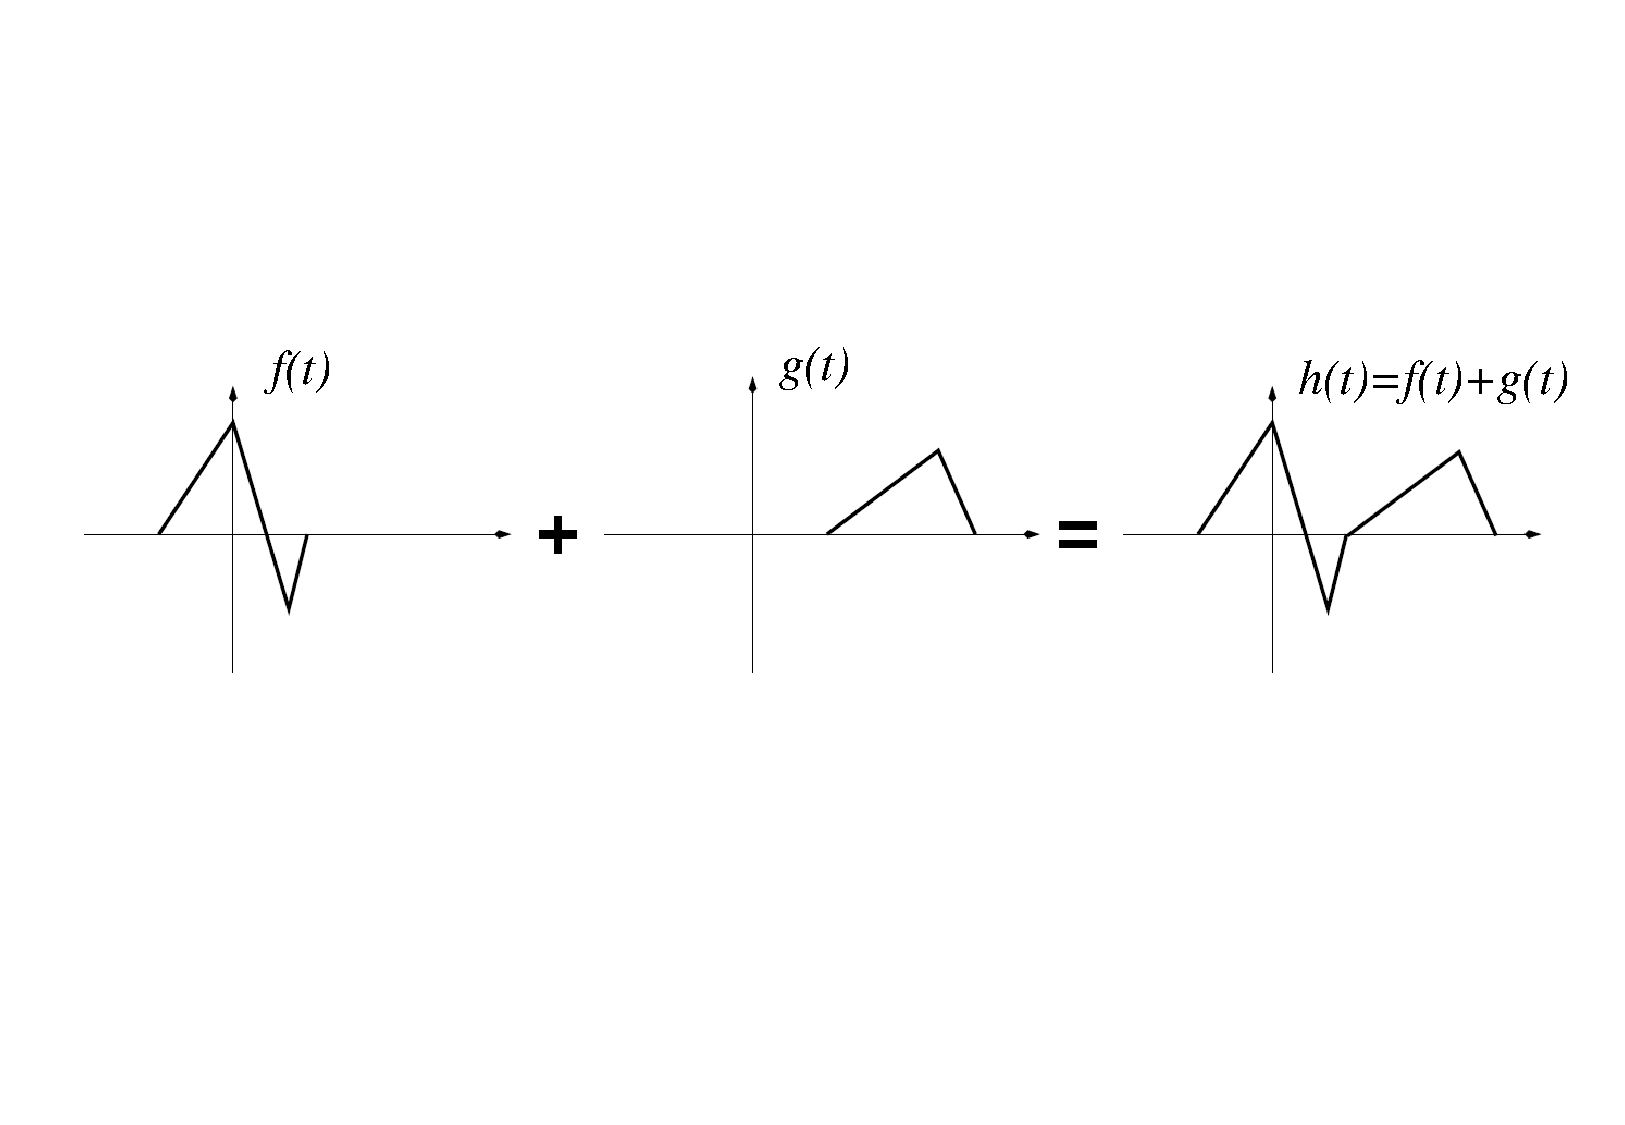
\includegraphics[width=1\textwidth]{img/op_somma_1.pdf}
		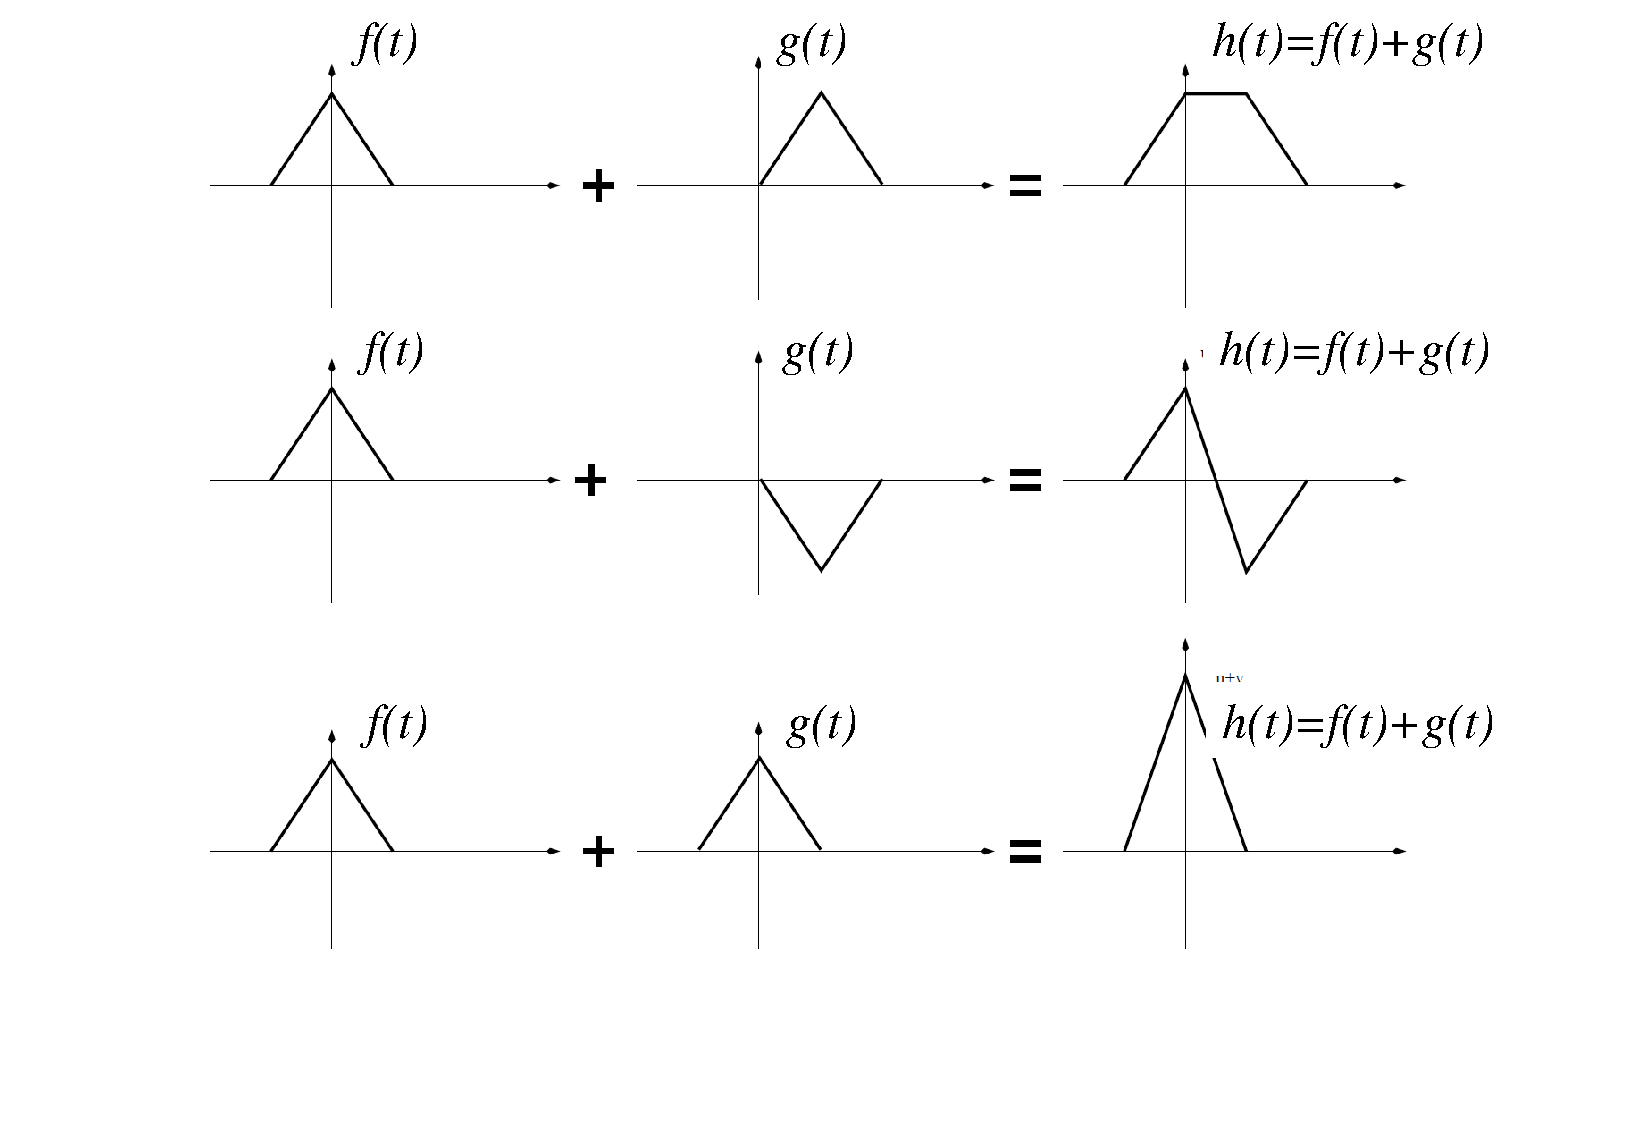
\includegraphics[width=1\textwidth]{img/op_somma_2.pdf}
	\end{figure}

	\newpage
	
	\subsubsection{Shift (o traslazione)}
	
	Lo \textbf{\emph{shift}} (o traslazione) è il cambio di posizione di un segnale. Può essere effettuato:
	
	\begin{itemize}
		\item \textbf{Traslazione a destra} con la funzione $f(t-\tau)$
		\item \textbf{Traslazione a sinistra} con la funzione $f(t+\tau)$
	\end{itemize}
	
	\begin{figure}[!htp]
		\centering
		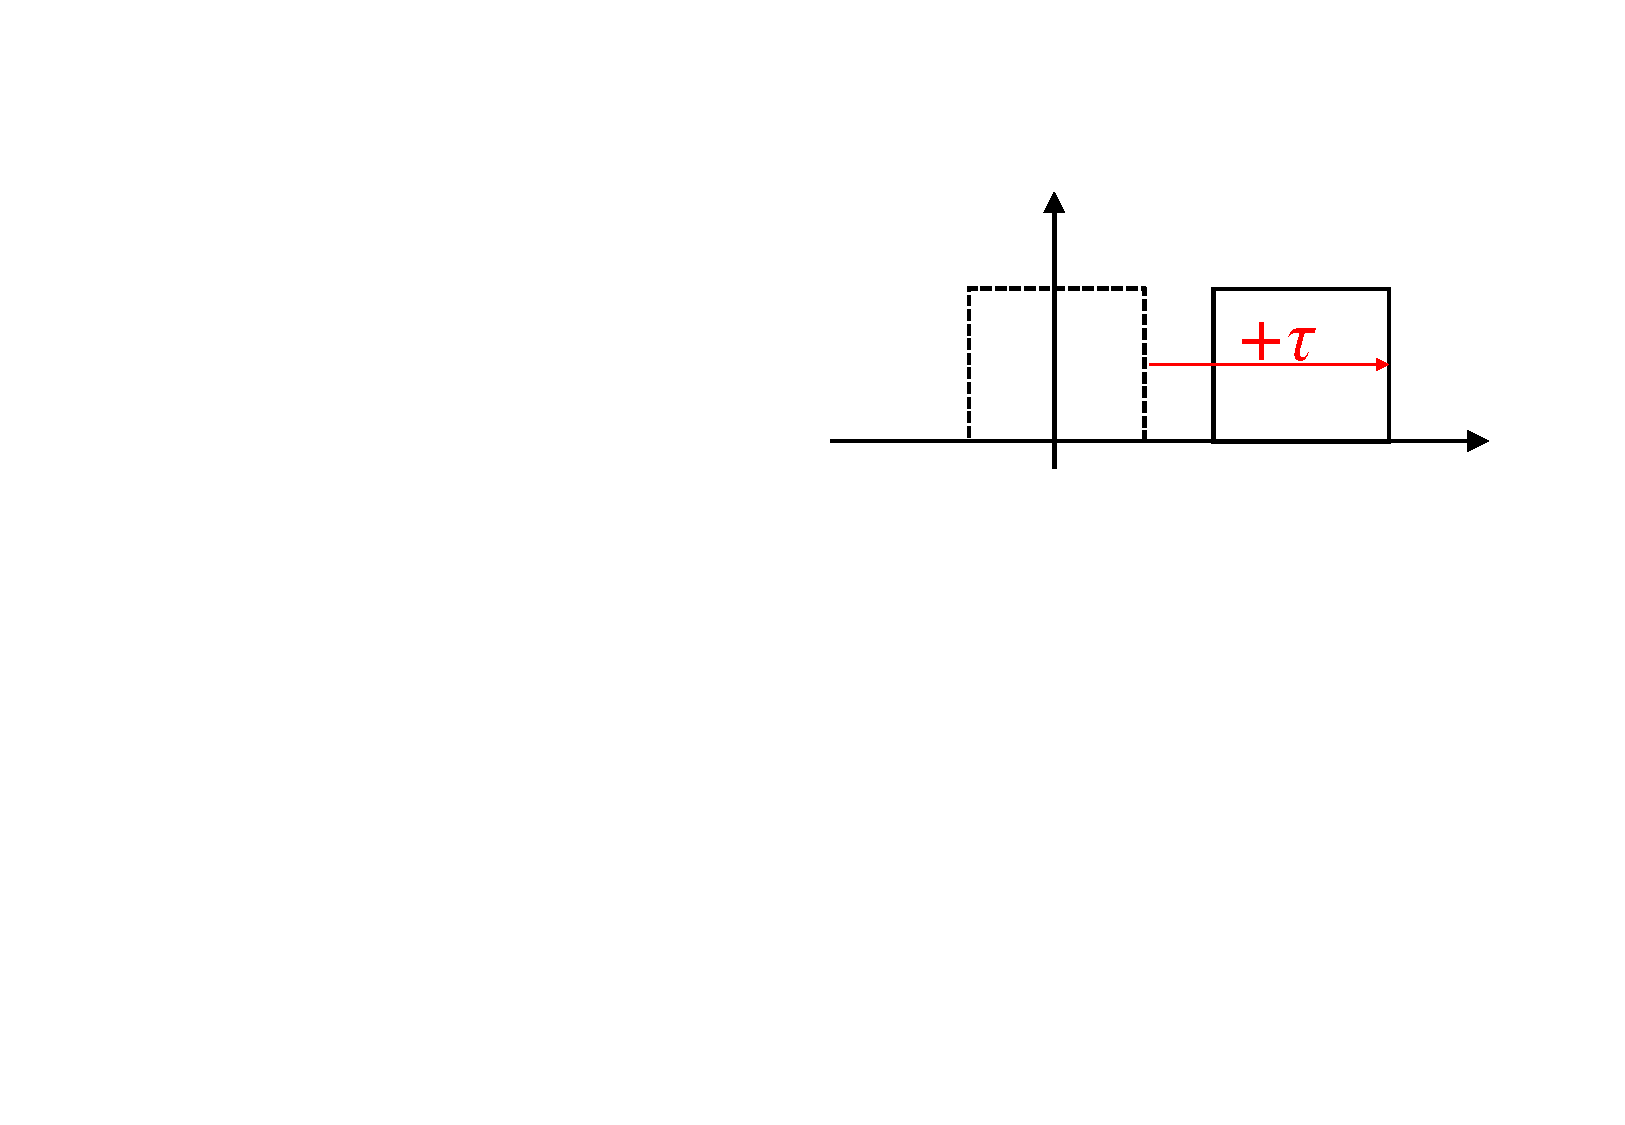
\includegraphics[width=0.5\textwidth]{img/op_shift_dx.pdf}\label{op_shift_dx}
		\caption{Shift a destra}
		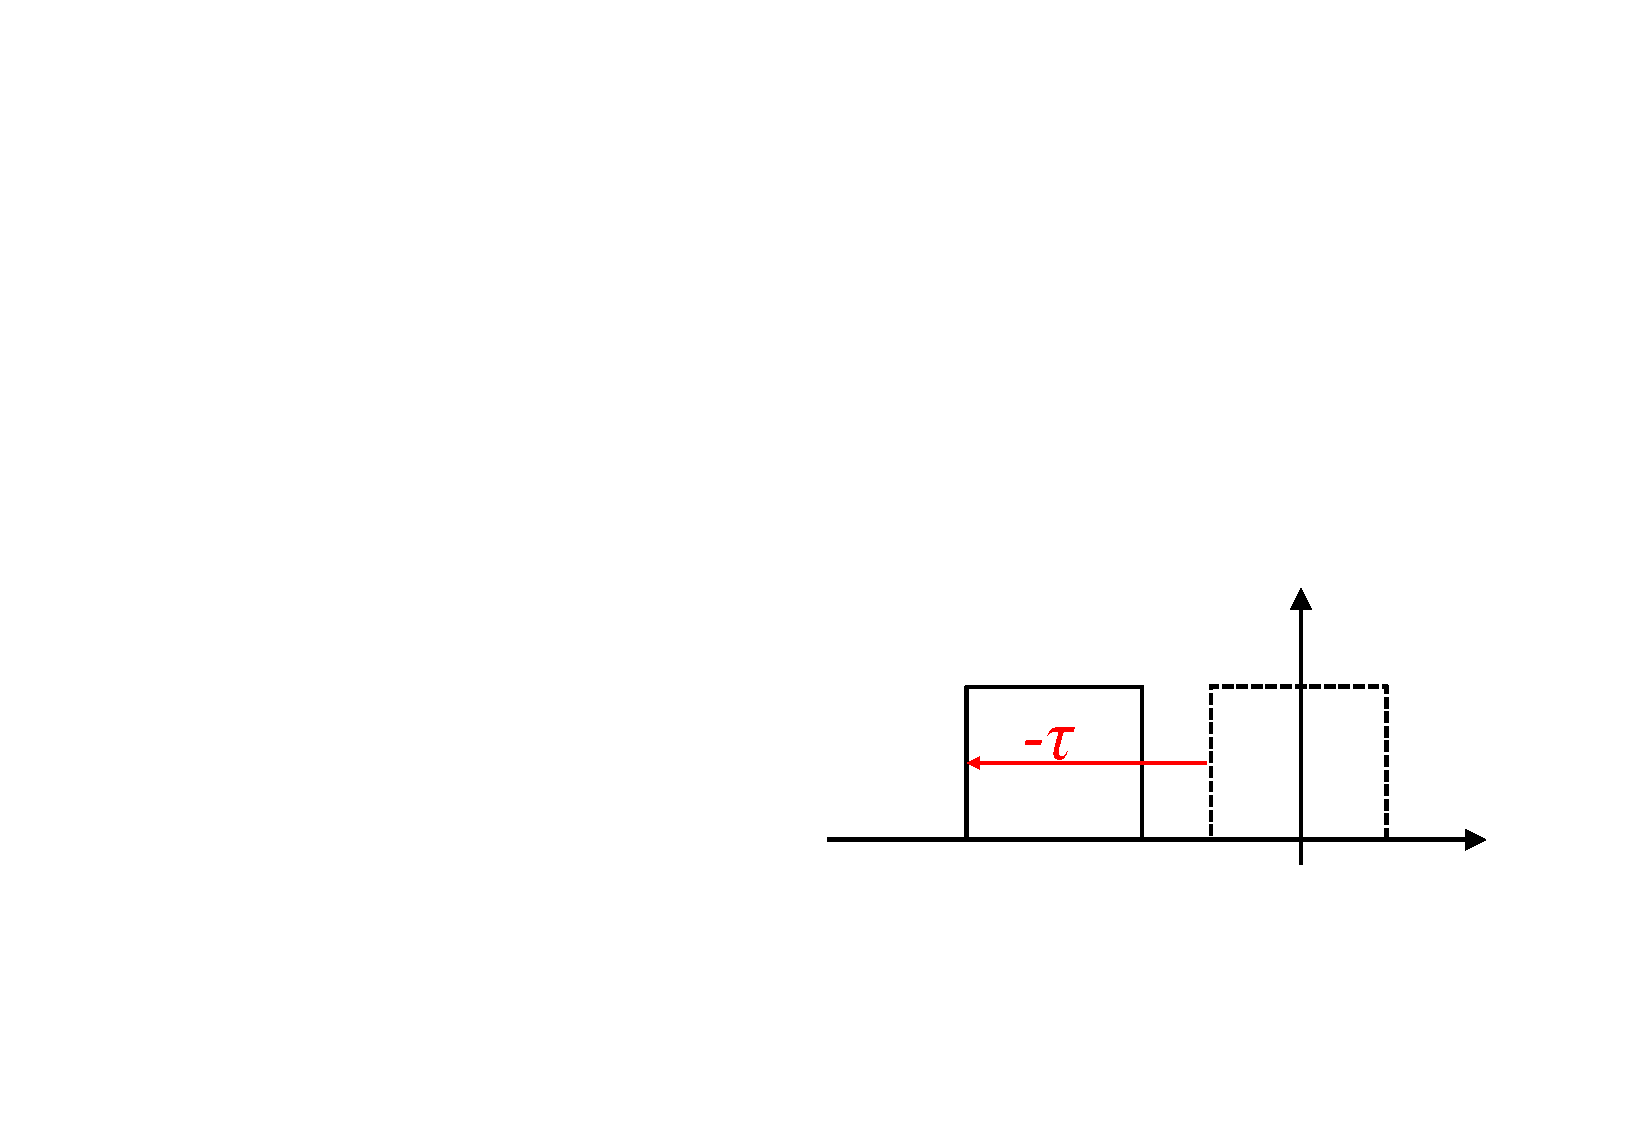
\includegraphics[width=0.5\textwidth]{img/op_shift_sx.pdf}\label{op_shift_sx}
		\caption{Shift a sinistra}
	\end{figure}

	\newpage
	
	\subsubsection{Funzione box $\Pi$ e impulso di Dirac}\label{funzione box e impulso di Dirac}
	
	La funzione \textbf{\emph{box}} è definita nel seguente modo:
	
	\begin{equation*}
		A \Pi\left(\dfrac{x}{b}\right) \hspace{2em} x\in\left[-\dfrac{b}{2}, \dfrac{b}{2}\right]
	\end{equation*}

	\begin{figure}[!htp]
		\centering
		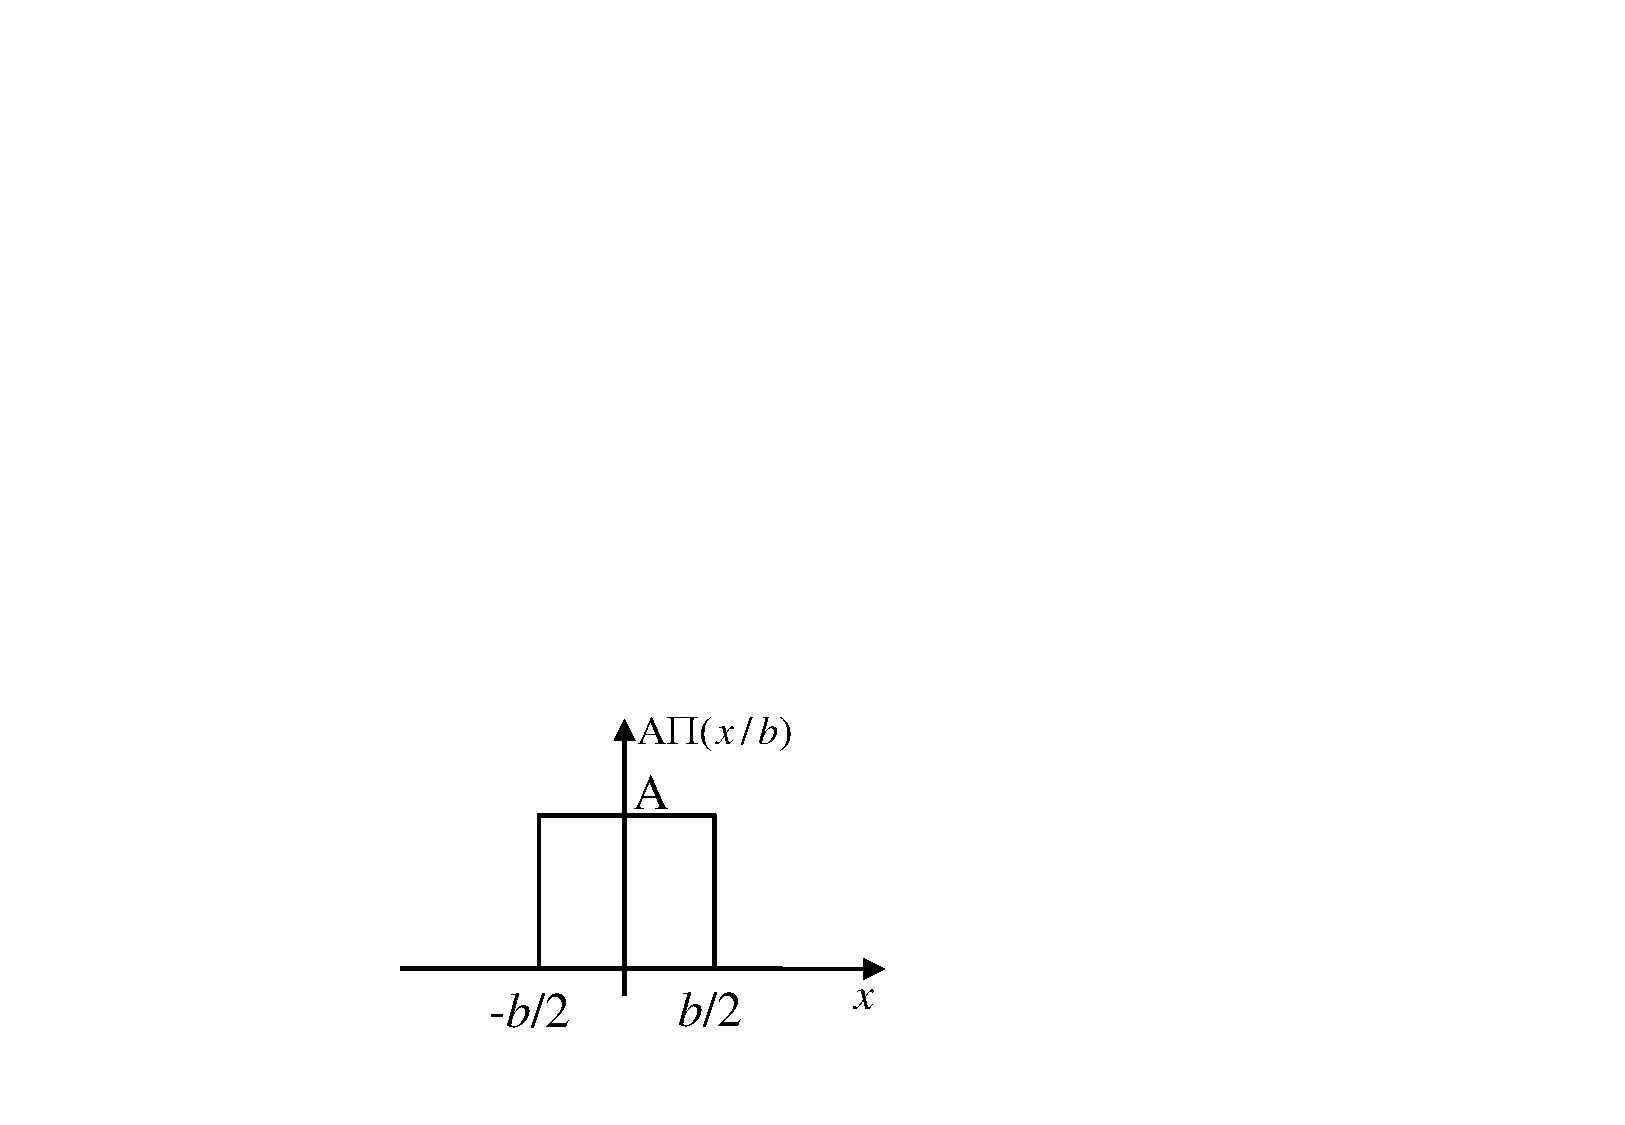
\includegraphics[width=0.4\textwidth]{img/box.pdf}\label{box}
		\caption{Box generica}
	\end{figure}

	La funzione $\delta(x)$ è chiamata \textbf{\emph{impulso unitario}} o \textbf{\emph{impulso di Dirac}} perché è definita nel seguente modo:
	
	\begin{equation*}
		\delta(x) = 
		\begin{cases}
			\infty  & \text{se } x=0 \\
			0		& \text{se } x\ne 0
		\end{cases}
		\hspace{2em} \int_{-\infty}^{\infty} \delta(x)\: dx = 1
	\end{equation*}

	\noindent
	Quindi è un impulso che tende all'infinito solamente quando la $x$ è nell'origine, ma il suo integrale è uguale a $1$. Alcune \textbf{proprietà} dell'impulso:
	
	\begin{enumerate}
		\item $\delta(x-x_0) = 0 \hspace{1em} \forall x\ne x_0$
		\item Data una funzione generica $f$ (\textbf{setacciamento}\label{setacciamento}): $\displaystyle \int_{-\infty}^{\infty} f(x)\delta(x-x_0)\: dt = f(x_0)$
		\item $\delta(x - x_0) = \delta(x_0 - x)$
		\item $\delta(ax) = \dfrac{1}{|a|} \delta(x) \hspace{1em} \forall x \in \mathbb{R} \text{, fissato } a \in \mathbb{R}-\{0\}$
	\end{enumerate}

	\newpage
	
	\subsubsection{Funzione sinc}\label{funzione sinc}
	
	La funzione \textbf{\emph{sinc}} è definita nel seguente modo:
	
	\begin{equation*}
		\mathrm{sinc}(t) = \dfrac{\sin{\left(\pi t\right)}}{\pi t}
	\end{equation*}

	\noindent
	Ha due \textbf{caratteristiche} importanti: (1) l'intersezione con l'asse delle $x$ avviene sempre nei numeri interi positivi e negativi (quindi $1$ e $-1$, $2$ e $-2$, ecc.); (2) il limite $\displaystyle \lim_{t\rightarrow \pm\infty}\mathrm{sinc}(t) = 0$.\newline
	Questa funzione è \textbf{importante per l'analisi nel dominio del tempo} (o \textbf{frequenza}).
	
	\subsubsection{Funzione triangolo $\Lambda$}
	
	La funzione \textbf{\emph{triangolo}} è definita nel seguente modo:
	
	\begin{equation*}
		\Lambda(x) =
		\begin{cases}
			1-|x|, 	& |x| < 1 \\
			0		& \text{altrimenti}
		\end{cases}
	\end{equation*}

	\noindent
	Questa funzione è \textbf{importante per l'analisi spettrale e} per le \textbf{operazioni di convoluzione}.
	
	\subsubsection{Funzione segno ($sgn$)}
	
	La funzione \textbf{\emph{segno}} è definita nel seguente modo:
	
	\begin{equation*}
		\mathrm{sgn}(x) =
		\begin{cases}
			-1, 	& x < 0 \\
			+1,		& x > 0 \\
			0		& x = 0
		\end{cases}
	\end{equation*}
	
	\noindent
	Questa funzione ribalta segnali sopra o sotto l'asse delle $x$.
	
	\subsubsection{Funzione gradino}
	
	La funzione \textbf{\emph{gradino}} è definita nel seguente modo:
	
	\begin{equation*}
		u(x) =
		\begin{cases}
			0 & x < 0 \\
			1 & x \ge 0
		\end{cases}
	\end{equation*}
	
	\noindent
	Questa funzione rappresenta un \textbf{segnale} che si attiva a partire dal tempo specificato e rimane attivo indefinitamente. Attenzione! Non si confonda questo segnale con il segno.
	
	\newpage
	
	\subsubsection{Treno di impulsi}
	
	Il \textbf{\emph{treno di impulsi}} $S_{\Delta T}(x)$ è la somma di un numero infinito di impulsi periodici discreti distanziati di una quantità $\Delta T$:
	
	\begin{equation*}
		S_{\Delta T}(x) = \sum_{n = -\infty}^{\infty} \delta (x - n \Delta T) \hspace{1em} n \in \mathbb{Z}
	\end{equation*}

	\begin{figure}[!htp]
		\centering
		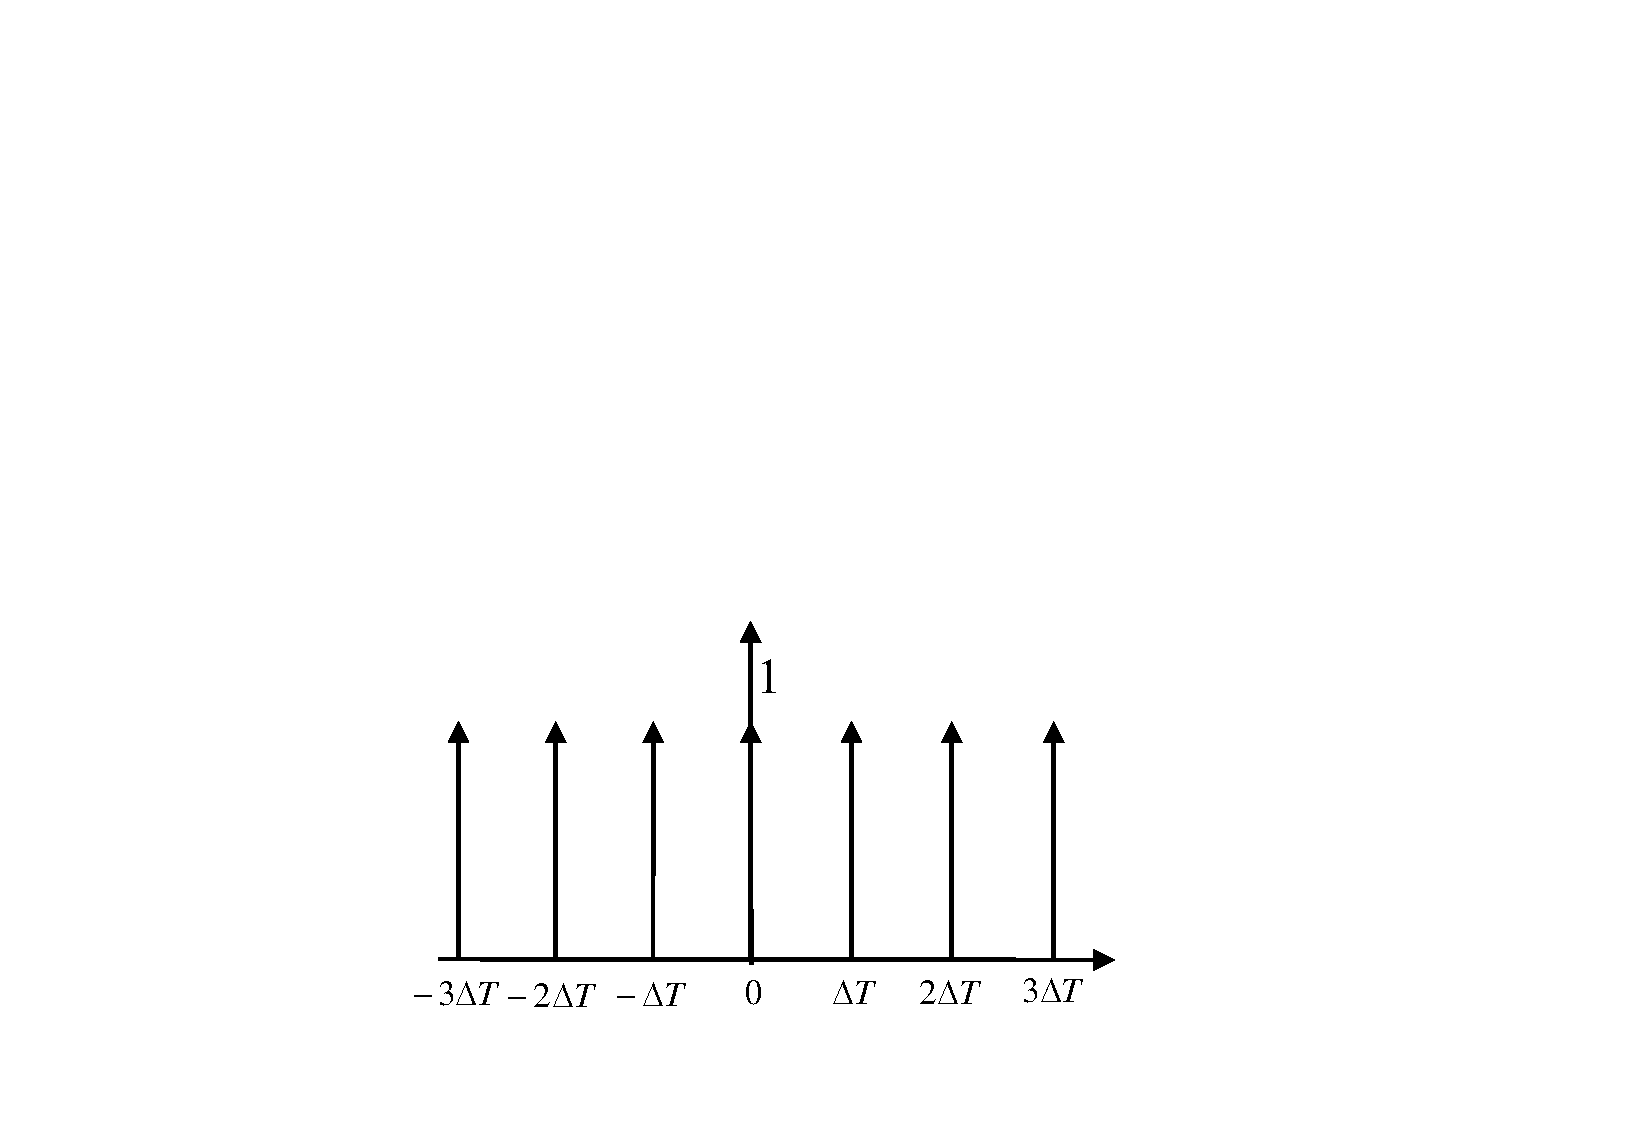
\includegraphics[width=0.5\textwidth]{img/treno_di_impulsi.pdf}\label{treno_di_impulsi}
		\caption{Treno di impulsi}
	\end{figure}

	\subsubsection{Energia di un segnale}
	
	L'\textbf{\emph{energia di un segnale}} è definita nel seguente modo:
	
	\begin{equation*}
		E_f =
		\begin{cases}
			\displaystyle \int_{-\infty}^{+\infty} f^{2}(t)\: dt & \text{se } f \in \mathbb{R} \\
			\displaystyle \int_{-\infty}^{+\infty} \left| f(t) \right|^{2} dt \hspace{1em} \text{con } \left| f(t) \right|^{2} = \tilde{f}(t) f(t), & f \in \mathbb{C}
		\end{cases}
	\end{equation*}
	
	\noindent
	Un segnale si dice \textbf{ad energia finita} (o \textbf{di energia}) se l'integrale che rappresenta l'energia converge ed è diverso da $0$. Quindi:
	
	\begin{itemize}
		\item[\ding{43}] \textbf{Condizione \emph{sufficiente}} all'esistenza della sua trasformata di Fourier. Le funzioni trigonometriche non sono di energia ma hanno comunque la Trasformata di Fourier.
		\item[\ding{42}] \textbf{Condizione \emph{necessaria}} per essere un segnale ad energia finita, all'infinito ($+\infty$ e $-\infty$) l'\textbf{ampiezza} va a zero.
	\end{itemize}

	\noindent
	Alcuni esempi:

	\begin{itemize}
		\item[\ding{80}] \textbf{Segnali di energia.} Impulsi rettangolari, oscillazioni smorzate ($\mathrm{sinc}$);
		\item[\ding{80}] \textbf{Segnali \underline{non} di energia.} Funzioni trigonometriche $\sin$ e $\cos$.
	\end{itemize}

	\noindent
	L'\textbf{unità di misura} è il \emph{joule}.
	
	\subsubsection{Potenza media di un segnale}
	
	La \textbf{\emph{potenza media di un segnale}} è definita nel seguente modo:
	
	\begin{equation*}
		P_f =
		\begin{cases}
			\displaystyle \lim_{T \rightarrow +\infty} \dfrac{1}{T} \int_{-\dfrac{T}{2}}^{+\dfrac{T}{2}} f^{2}(t)\: dt & \text{se } f \in \mathbb{R} \\
			\displaystyle \lim_{T \rightarrow +\infty} \dfrac{1}{T} \int_{-\dfrac{T}{2}}^{+\dfrac{T}{2}} \left|f(t)\right|^{2}\: dt \hspace{1em} \text{con } \left| f(t) \right|^{2} = \tilde{f}(t) f(t), & f \in \mathbb{C}
		\end{cases}
	\end{equation*}
	
	\noindent
	Un segnale si dice \textbf{a potenza finita} (o \textbf{di potenza}) se l'integrale che rappresenta la potenza converge ed è diverso da $0$. L'\textbf{unità di misura} è il \emph{watt}.\newline
	Infine, un segnale ad energia finita ha la potenza che tende a zero (per cui un segnale non può appartenere ad entrambe le categorie). Invece, esistono segnali che non sono né di energia, n* di potenza finita.
	
	\newpage
	
	\subsection{Altre operazioni fondamentali}
	
	\subsubsection{Rescaling (o riscalatura)}
	
	La funzione di \textbf{\emph{rescaling}} è definita nel seguente modo:
	
	\begin{equation*}
		\forall f(t) : D_1 \in \mathbb{R}, \hspace{1em} \omega \ne 0
	\end{equation*}
	
	\noindent
	Simile allo \emph{shift}, il \emph{rescaling} ha una definizione generica e due varianti:
	
	\begin{itemize}
		\item \textbf{Definizione generica} con la funzione semplice $f(t)$ (immagine~\ref{rescaling}).
		\item \textbf{Ritardo \underline{lineare} del segnale di un fattore $\omega$} con la funzione $f(\omega t), 0 < \omega < 1$ (immagine~\ref{rescaling_ritardo}).
		\item \textbf{Accelero \underline{lineare} del segnale di un fattore $\omega$} con la funzione $f(\omega t), \omega > 1$ (immagine~\ref{rescaling_accelero}).
	\end{itemize}
	
	\begin{figure}[!htp]
		\centering
		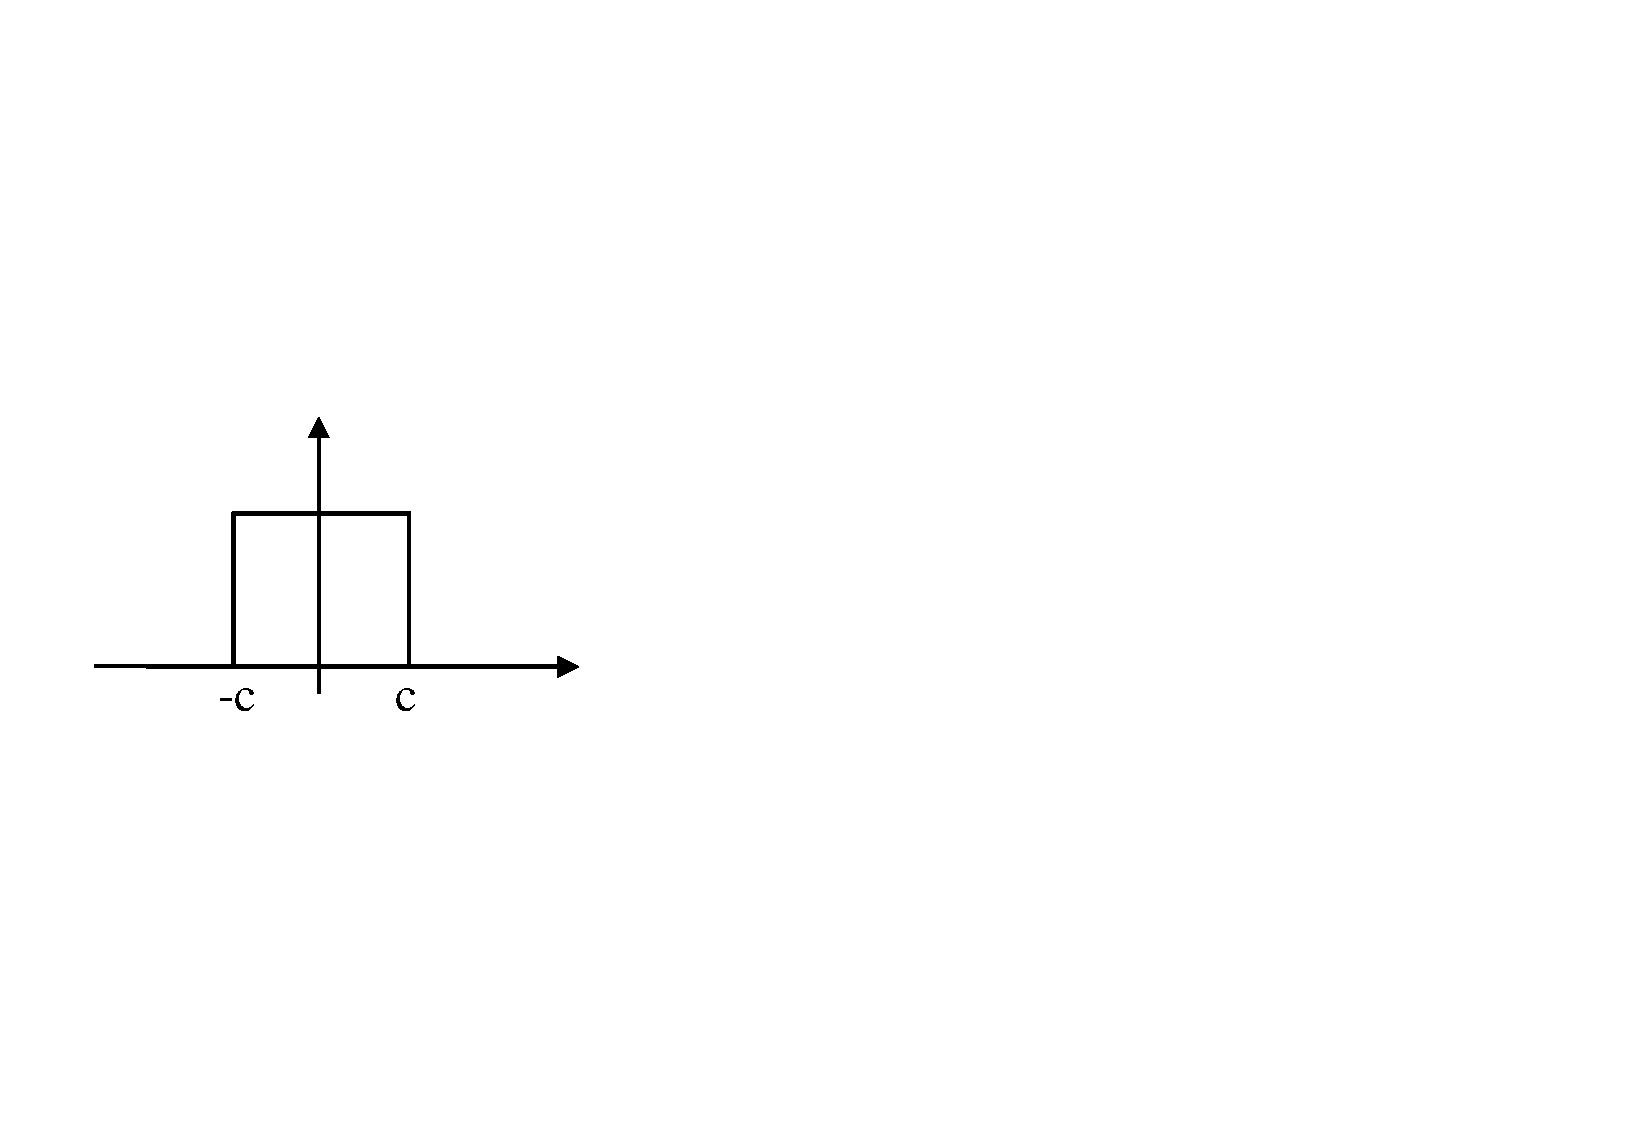
\includegraphics[width=0.5\textwidth]{img/rescaling.pdf}
		\caption{Definizione generica}\label{rescaling}
		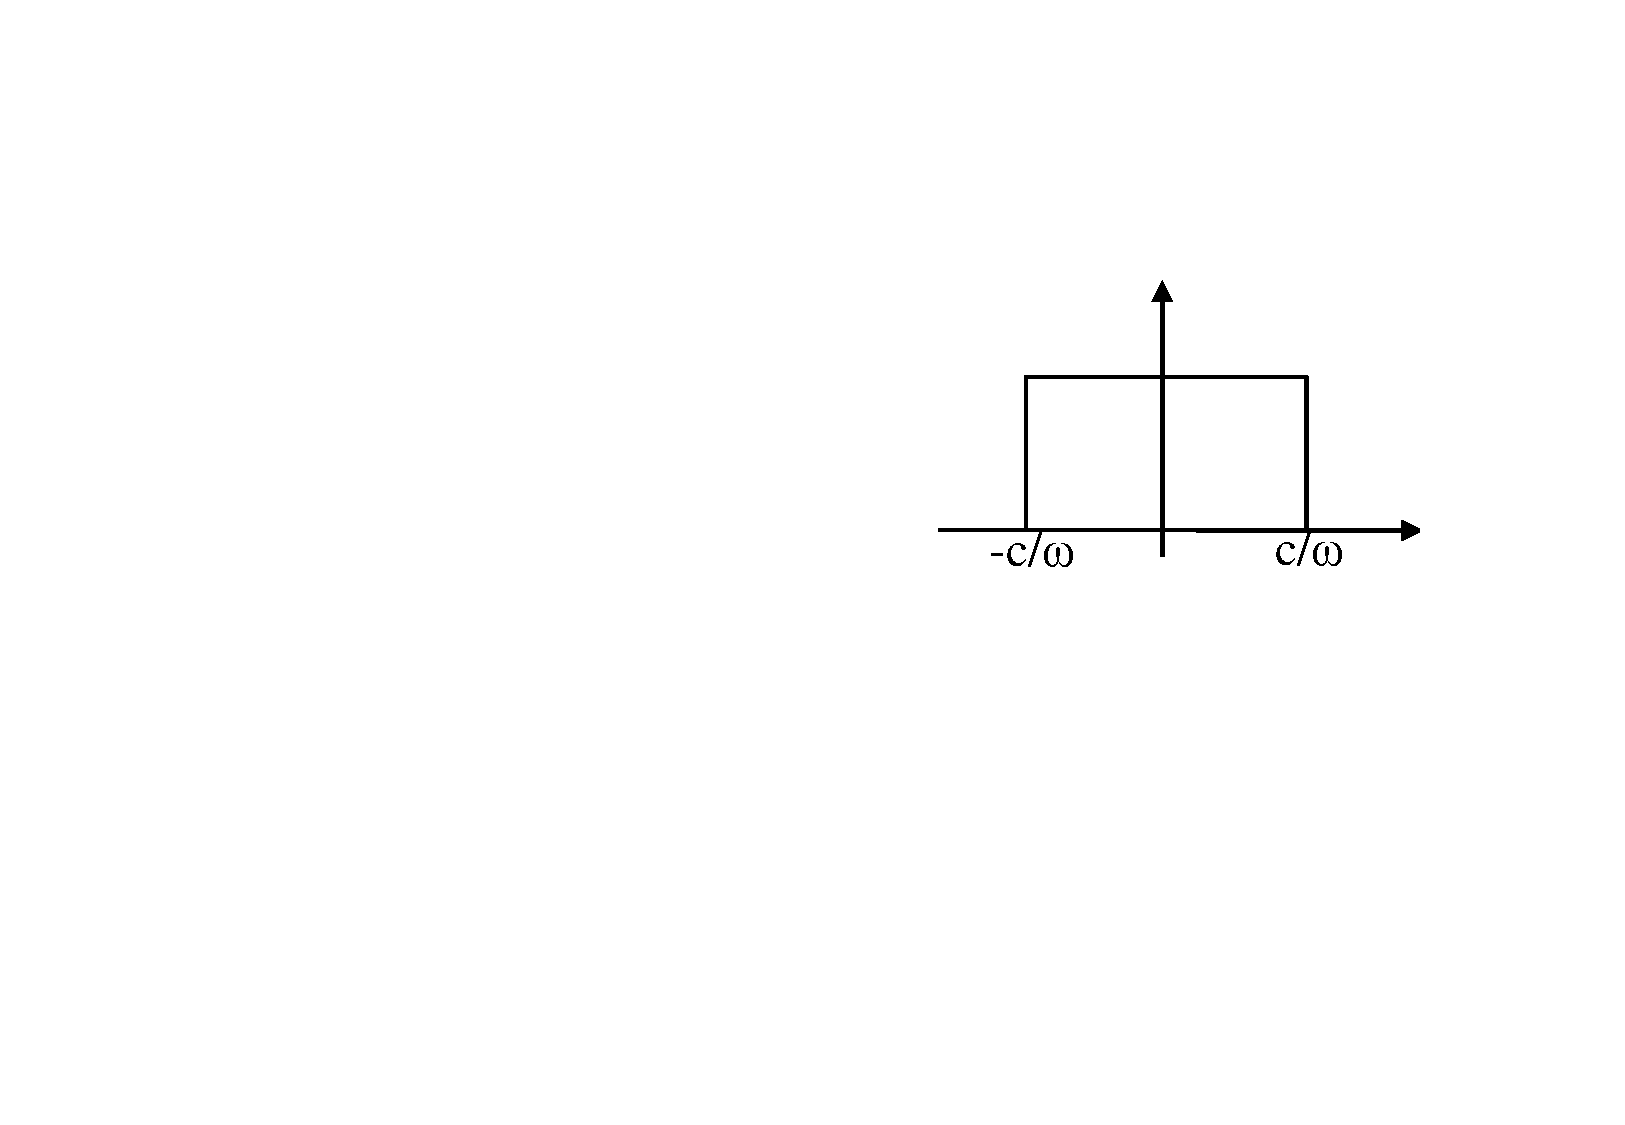
\includegraphics[width=0.5\textwidth]{img/rescaling_ritardo.pdf}
		\caption{Ritardo \underline{lineare} del segnale di un fattore $\omega$}\label{rescaling_ritardo}
		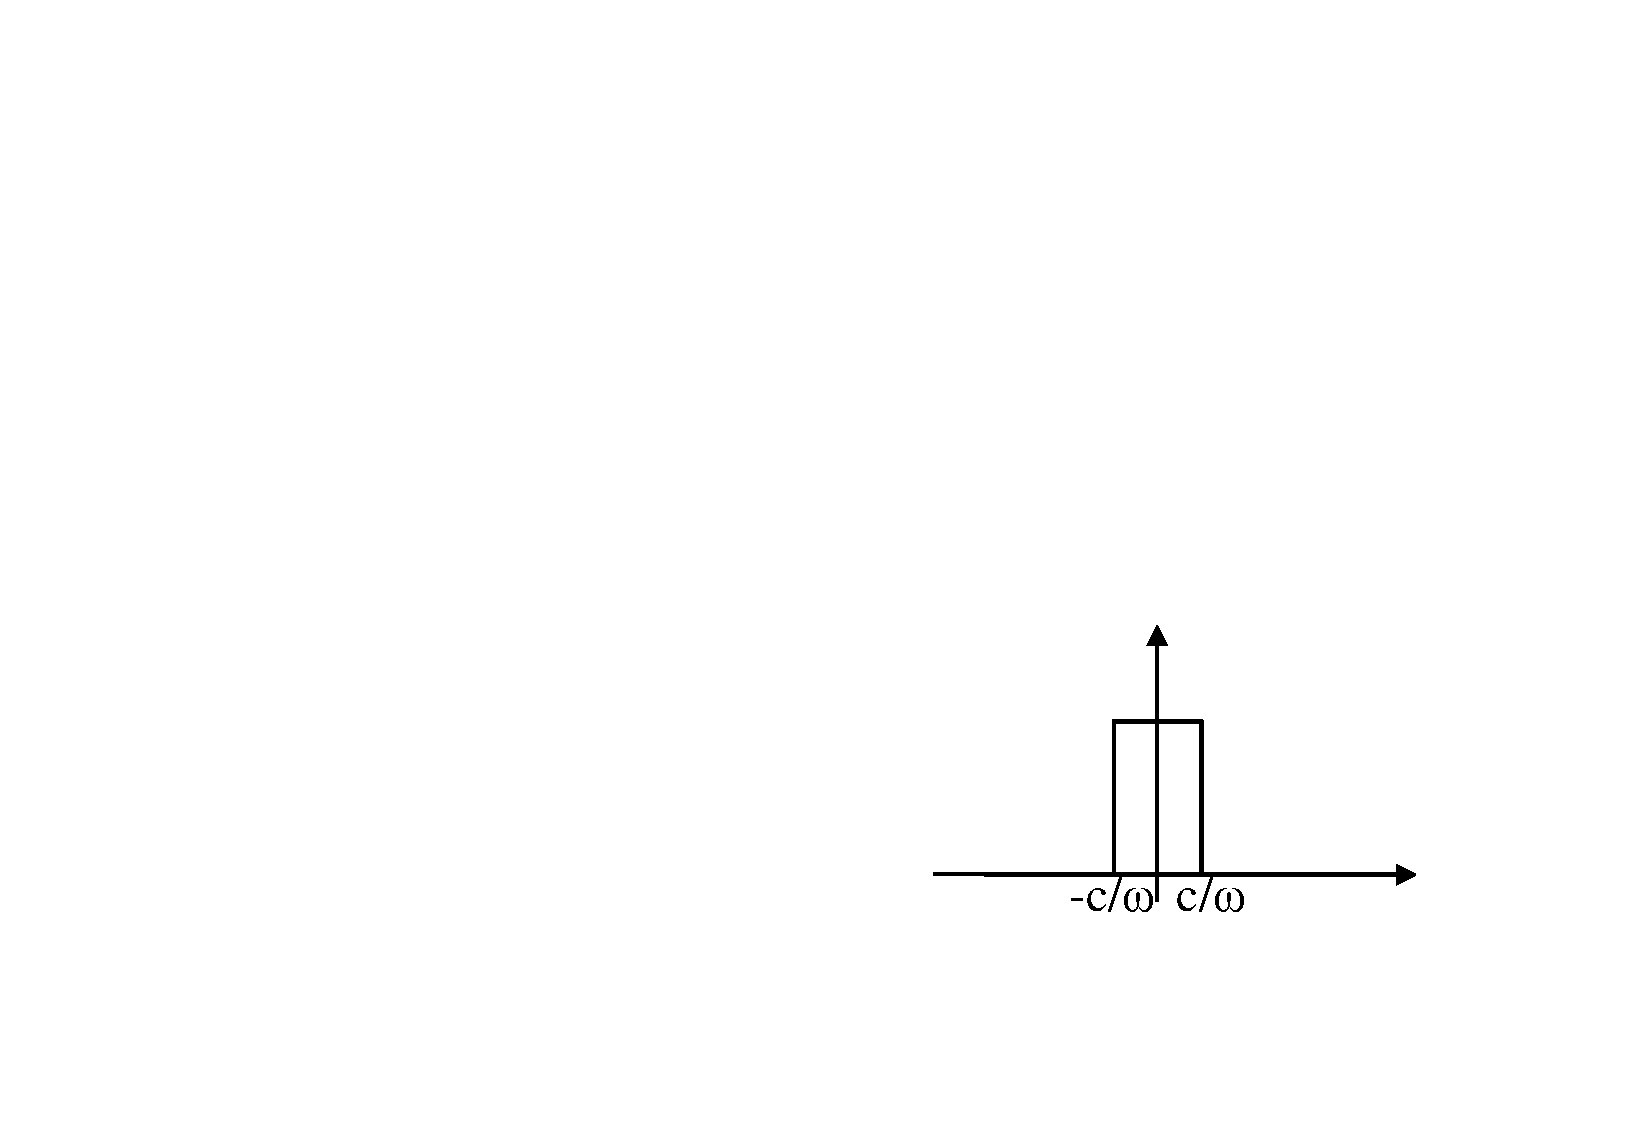
\includegraphics[width=0.5\textwidth]{img/rescaling_accelero.pdf}
		\caption{Accelero \underline{lineare} del segnale di un fattore $\omega$}\label{rescaling_accelero}
	\end{figure}

	\subsubsection{Cross-Correlazione}
	
	Dati $f_1(\tau), f_2(\tau)$ segnali continui, $\tau\in\mathbb{R}$ il segnale di \textbf{\emph{cross-correlazione}} viene definito come:
	
	\begin{equation*}
		\displaystyle f_1 \otimes f_2 (t) = \int_{-\infty}^{+\infty} \tilde{f_1}(\tau) f_2(\tau - t)\: d\tau
	\end{equation*}

	\noindent
	In cui $\tilde{f_1}(\tau)$ rappresenta un \emph{complesso coniugato}. Nel caso in cui $f_1$ è reale, allora $\tilde{f_1}(\tau) \rightarrow f_1(\tau)$. \newline
	Infine, con $t = 0$ si ha l'\textbf{\emph{integrale di cross-correlazione}}, il quale è definito se l'integrale converge (ovviamente se il segnale non è né di energia, né di potenza, la convergenza non esiste!).
	
	\newpage
	
	
	
	
	\subsubsection{Esercizi d'esame}
	
	\textcolor{Red3}{\textbf{\emph{Esercizio.}}}
	
	Il primo esercizio fornisce una funzione $f(t)$:
	
	\begin{equation*}
		f(t) = \Pi \left(\dfrac{t-2}{4}\right) e^{-2t}
	\end{equation*}

	\noindent
	Le \textbf{richieste} dell'esercizio sono le seguenti:
	
	\begin{enumerate}[label=\Roman*]
		\item Rappresentare graficamente il segnale;
		
		\item Calcolare sia l'energia che la potenza media. Inoltre, dire se $f(t)$ è una funzione di energia o di potenza fornendo una motivazione valida. Infine, calcolare l'energia o la potenza nel caso in cui $f(t)$ sia solo composta da $e^{-2t}$;
		
		\item Scrivere l'espressione analitica rispetto $z(t) = -f(-t)$ e $v(t) = f(t+4)$
	\end{enumerate}

	\noindent
	\textcolor{Green4}{\textbf{\emph{Risoluzione I.}}}
	
	\noindent
	Il \textbf{primo passo} è quello di scomporre la funzione così da avere una visione più chiara sulle operazioni da effettuare:
	
	\begin{equation*}
		f(t) = \Pi \left(\dfrac{t-2}{4}\right) e^{-2t} \longrightarrow f(t) = \Pi \left(\dfrac{1}{4} \cdot \left(t - 2\right)\right)
	\end{equation*}

	\noindent
	Come si può osservare, ci sono due operazioni da eseguire. Quindi, dopo l'esplicitazione si esegue la rappresentazione del segnale base $\Pi(t)$:
	
	\begin{figure}[!htp]
		\centering
		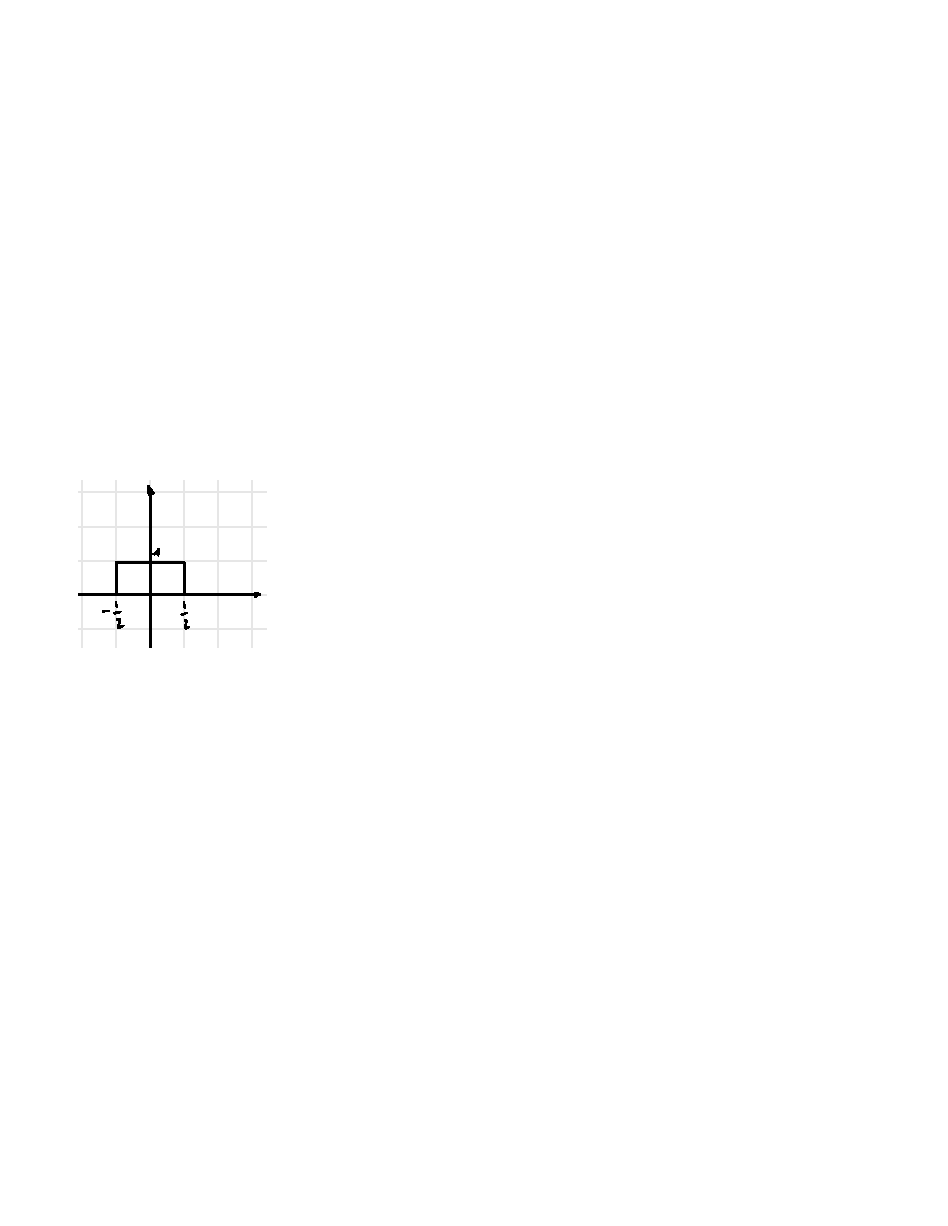
\includegraphics[width=0.4\textwidth]{img/ex_exam/Pi_func_1.pdf}
		\caption{Rappresentazione della funzione $f(t)$, ovvero un box.}
	\end{figure}

	\newpage
	Adesso si esegue l'operazione di moltiplicazione per un fattore che in questo caso è $\dfrac{1}{4}$. Quindi si rappresenta la box $\Pi\left(\dfrac{1}{4}\cdot t\right)$:
	
	\begin{figure}[!htp]
		\centering
		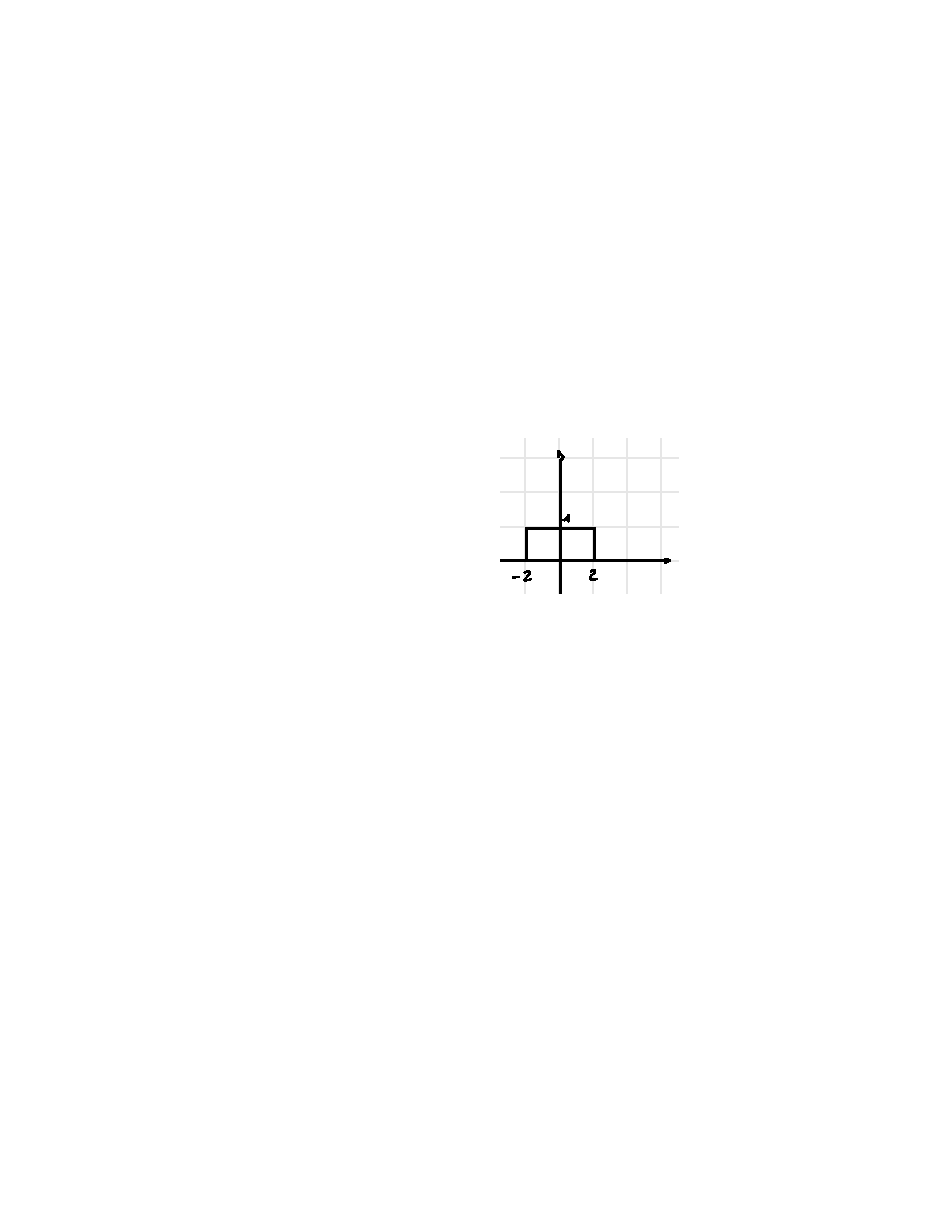
\includegraphics[width=0.4\textwidth]{img/ex_exam/Pi_func_1-Mod.pdf}
		\caption{Box $\Pi\left(\dfrac{1}{4}\cdot t\right)$ allargata.}
	\end{figure}

	\noindent
	L'operazione che è stata effettuata è stata semplicemente considerare la box del tipo $\Pi\left(\dfrac{t}{4}\right)$. Ricordandosi le nozioni del corso di Sistemi, per definizione quindi la box è definita nell'intervallo $-2, +2$.
	
	Infine, viene applicata l'ultima operazione, ovvero il $-2$ all'incognita $t$. Quindi, la funzione box diventerà $\Pi\left(\dfrac{1}{4}\left(t-2\right)\right)$ e la sua rappresentazione grafica sarà uno shift a destra (ritardo):
	
	\begin{figure}[!htp]
		\centering
		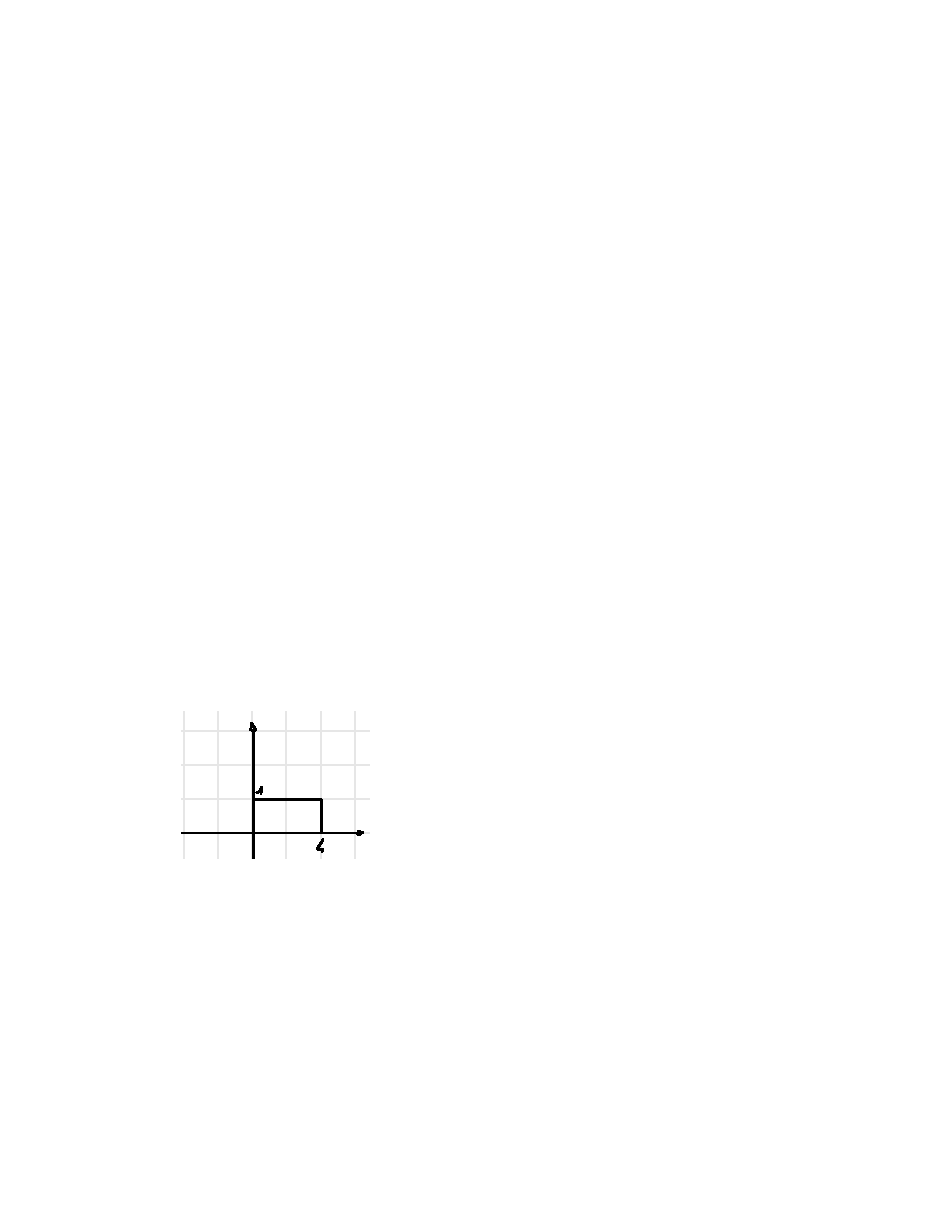
\includegraphics[width=0.4\textwidth]{img/ex_exam/Pi_func_1-Mod2.pdf}
		\caption{Box $\Pi\left(\dfrac{1}{4}\left(t-2\right)\right)$ dopo lo shift a destra.}
	\end{figure}

	\newpage

	Il \textbf{primo punto si conclude} con la rappresentazione del segnale $e^{-2t}$ e la sua combinazione con la box. Quindi:
	
	\begin{figure}[!htp]
		\centering
		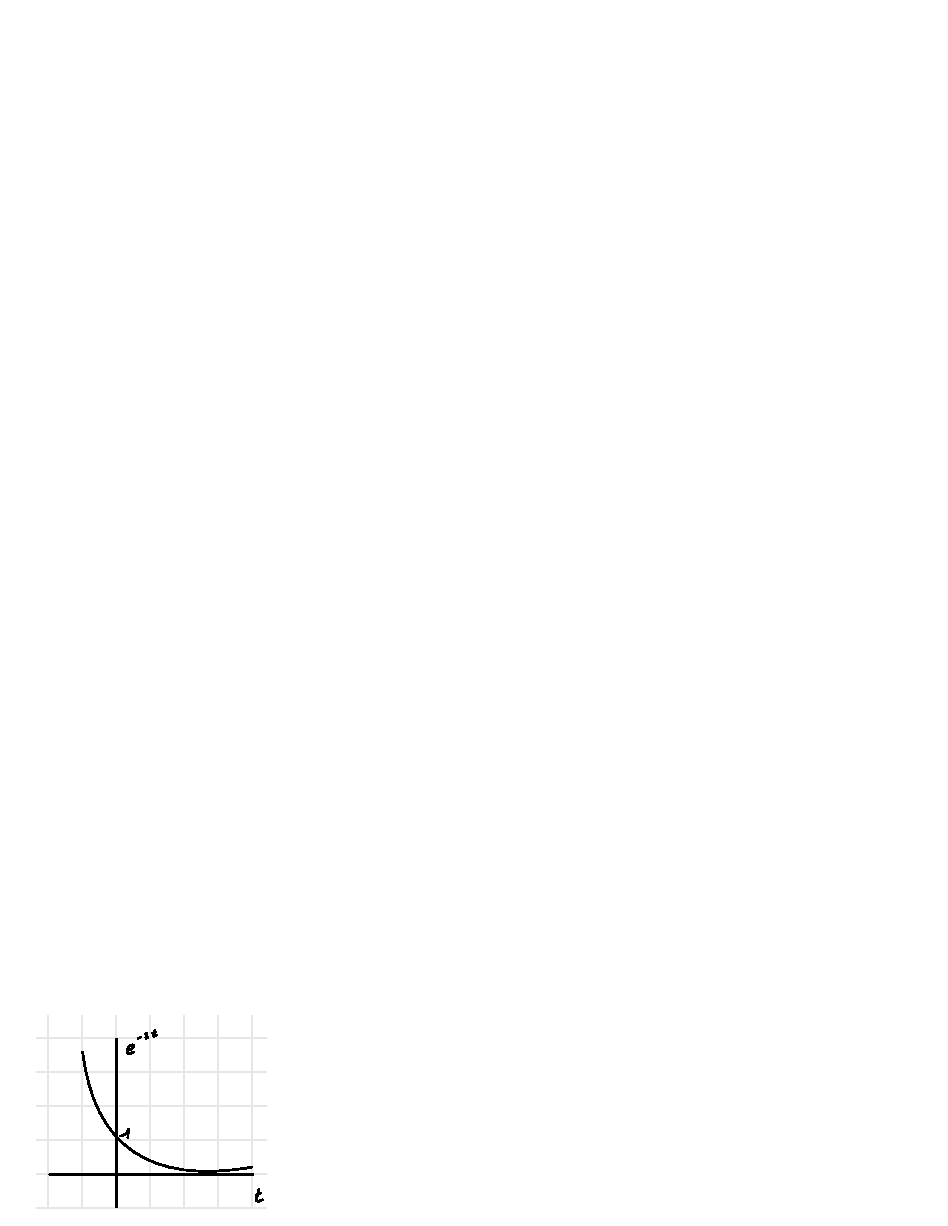
\includegraphics[width=0.4\textwidth]{img/ex_exam/E_func_1.pdf}
		\caption{Rappresentazione della funzione $e^{-2t}$}
	\end{figure}

	\noindent
	E infine la sua concatenazione con la box, quindi una sorta di applicazione di un filtro:
	
	\begin{figure}[!htp]
		\centering
		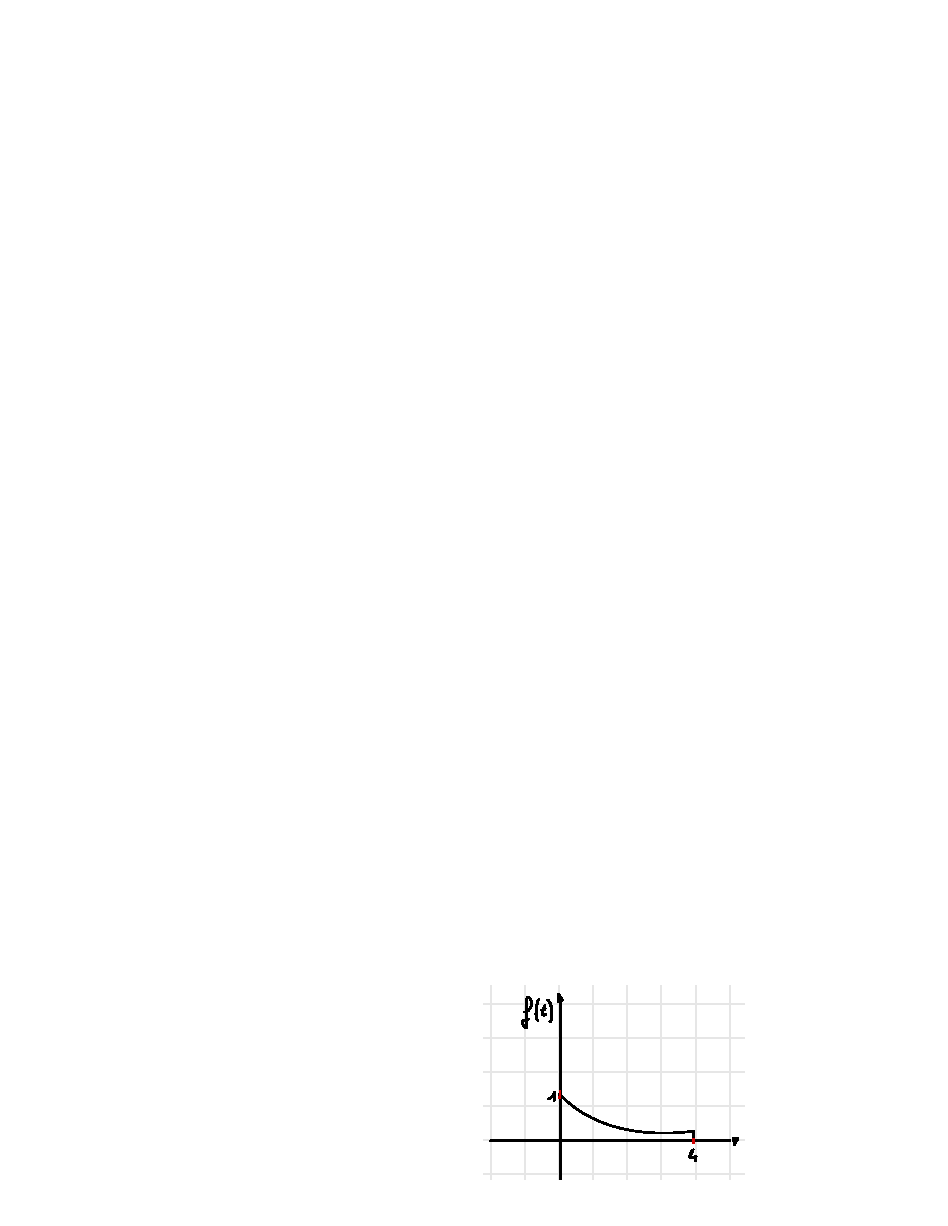
\includegraphics[width=0.4\textwidth]{img/ex_exam/Sol_func_1.pdf}
		\caption{Rappresentazione finale della funzione $f(t) = \Pi \left(\dfrac{t-2}{4}\right) e^{-2t}$}\label{ex1_grafico}
	\end{figure}

	\newpage

	\noindent
	\textcolor{Green4}{\textbf{\emph{Risoluzione II.}}}

	Guardando la figura~\ref{ex1_grafico} si può già intuire che tipo di segnale sia. Infatti, dato che è limitato e non si estende all'infinito, per definizione è un \textbf{segnale finito}, quindi \textbf{di energia} e \underline{non} di potenza. Per dimostrare questa affermazione, si eseguono i calcoli:
	
	\begin{gather*}
		\textbf{Definizione di energia: } E_{f} = \int_{-\infty}^{\infty}{\left|f(t)\right|^2\:\mathrm{d}t} = \int_{-\infty}^{\infty}{f(t)^2\:\mathrm{d}t} \\
		\textbf{Definizione di potenza: } P_{f} = \lim_{T\rightarrow\infty}{\dfrac{1}{T} \int_{-\frac{T}{2}}^{\frac{T}{2}}{f^{2}(t)\:\mathrm{d}t}}
	\end{gather*}

	\noindent
	Dopo le definizioni, si esegue l'effettivo calcolo con i valori numerici:
	
	\begin{gather*}
		\textbf{Energia finita} \\
		E_{f} = \int_{0}^{4}{e^{-4t}\:\mathrm{d}t} = \left.\dfrac{e^{-4t}}{-4}\right\vert_{0}^{4} = \dfrac{-e^{-16}+1}{4} = \dfrac{1}{4} \ne 0 \\
		\textbf{Potenza finita} \\
		P_{f} = \lim_{T\rightarrow\infty}{\dfrac{1}{T} \int_{0}^{4}{e^{-4t}\:\mathrm{d}t}} = \lim_{T\rightarrow\infty}{\dfrac{1}{T}\cdot\dfrac{1}{4}} = 0
	\end{gather*}

	\noindent
	Come si osserva dai risultati, \underline{è} un segnale di energia finita poiché è un valore noto, invece \underline{non è} un segnale di potenza poiché il risultato è zero e non rispetta la definizione.
	
	Al contrario, se la funzione fosse composta solamente dall'esponenziale, il calcolo dell'energia e della potenza sarebbe:
	
	\begin{gather*}
		\textbf{Energia: } E_{f} = \int_{-\infty}^{\infty}{e^{-4t}\:\mathrm{d}t} = \left.\dfrac{e^-4t}{-4}\right\vert_{-\infty}^{\infty} = \lim_{T\rightarrow\infty}{\dfrac{e^{-4t} - e^{4t}}{-4}} = \infty \\
		\textbf{Potenza: } P_{f} = \lim_{T\rightarrow\infty}{\dfrac{1}{T} \int_{-\frac{T}{2}}^{\frac{T}{2}}{e^{-4t}\:\mathrm{d}t}} = \lim_{T\rightarrow\infty}\left.\dfrac{e^{-4t}}{-4}\cdot\dfrac{1}{T}\right\vert_{-\frac{T}{2}}^{\frac{T}{2}} = \lim_{T\rightarrow\infty}\dfrac{e^{-2T} - e^{2T}}{-4T} = \infty
	\end{gather*}

	\noindent
	Come si evince dai calcoli, il segnale non è né di energia né di potenza perché entrambi i risultati sono uguali a infinito.\newline
	
	\noindent
	\textcolor{Green4}{\textbf{\emph{Risoluzione III.}}}
	
	Considerando la funzione $z(t)$, si osserva che è la copia simmetrica rispetto all'origine di $f(t)$. Invece, la funzione $v(t)$ è identica alla funzione $f(t)$ ma ``shiftata'' a sinistra di $4$:
	
	\begin{equation*}
		f(t) = -f(-t) \hspace{2em} v(t) = f(t + 4)
	\end{equation*}

	\newpage
	
	\noindent
	\textcolor{Red3}{\textbf{\emph{Esercizio 2.}}}
	
	\noindent
	Il secondo esercizio fornisce una funzione $f(t)$:
	
	\begin{equation*}
		f(t) = \mathrm{sgn }\left(a\cdot\cos{\left(\dfrac{2\pi}{T_0} t\right)}\right)
	\end{equation*}
	
	\noindent
	Con $T_0 = 2$. Le \textbf{richieste} dell'esercizio sono le seguenti:
	
	\begin{enumerate}[label=\Roman*]
		\item Rappresentare graficamente il segnale;
		
		\item Calcolare sia l'energia che la potenza media. Inoltre, dire se $f(t)$ è una funzione di energia o di potenza fornendo una motivazione valida.
	\end{enumerate}
	
	\noindent
	\textcolor{Green4}{\textbf{\emph{Risoluzione I.}}}
	
	\noindent
	Viene rappresentato il segnale della funzione segno $\mathrm{sng}$:
	
	\begin{figure}[!htp]
		\centering
		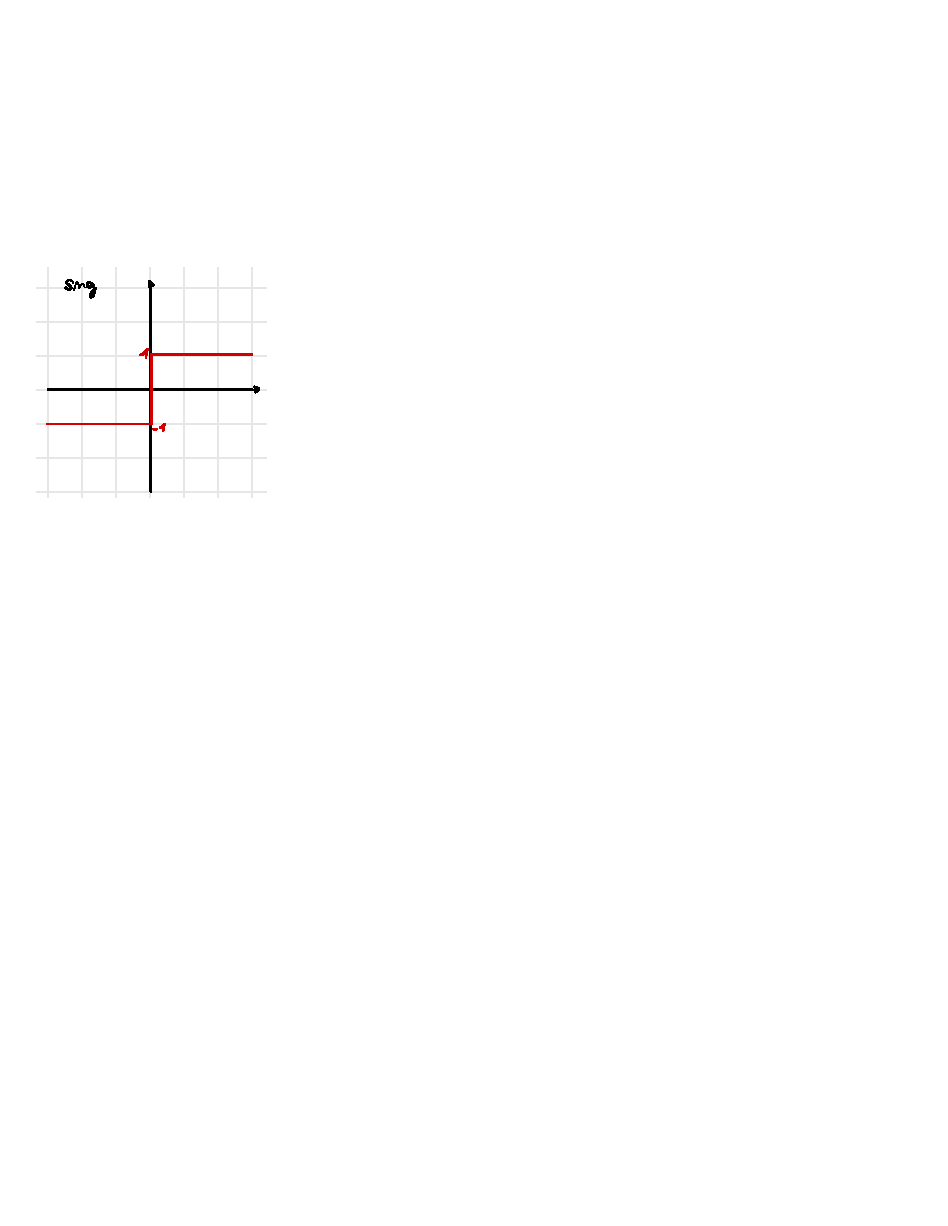
\includegraphics[width=0.4\textwidth]{img/ex_exam/sng_func_2.pdf}
		\caption{Funzione segno $\mathrm{sng}$.}
	\end{figure}

	\noindent
	Si esplicitando le operazioni della funzione:
	
	\begin{equation*}
		f(t) = \mathrm{sgn }\left(a\cdot\cos{\left(\dfrac{2\pi}{T_0} t\right)}\right) = \cos\left(\dfrac{1}{T_0}\cdot 2\pi t\right)
	\end{equation*}

	\noindent
	E si rappresenta inizialmente la funzione $\cos\left(2\pi\right)$ con $T_0 = 1$:
	
	\begin{figure}[!htp]
		\centering
		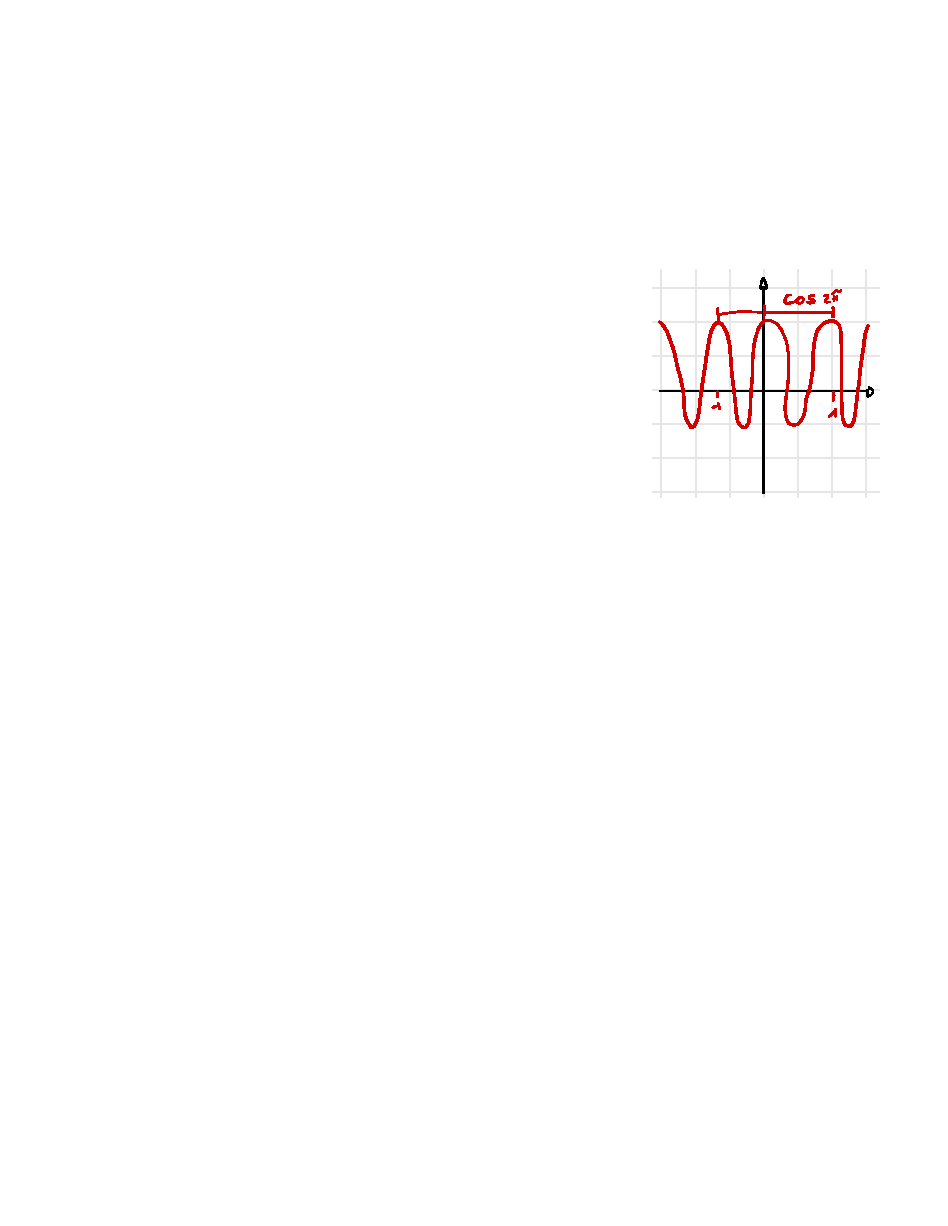
\includegraphics[width=0.4\textwidth]{img/ex_exam/sng_func_2-Mod.pdf}
		\caption{Funzione coseno $\cos\left(2\pi\right)$.}
	\end{figure}

	\newpage

	\noindent
	Si conclude la rappresentazione grafica aumentando $T_0$ in maniera molto semplice:
	
	\begin{figure}[!htp]
		\centering
		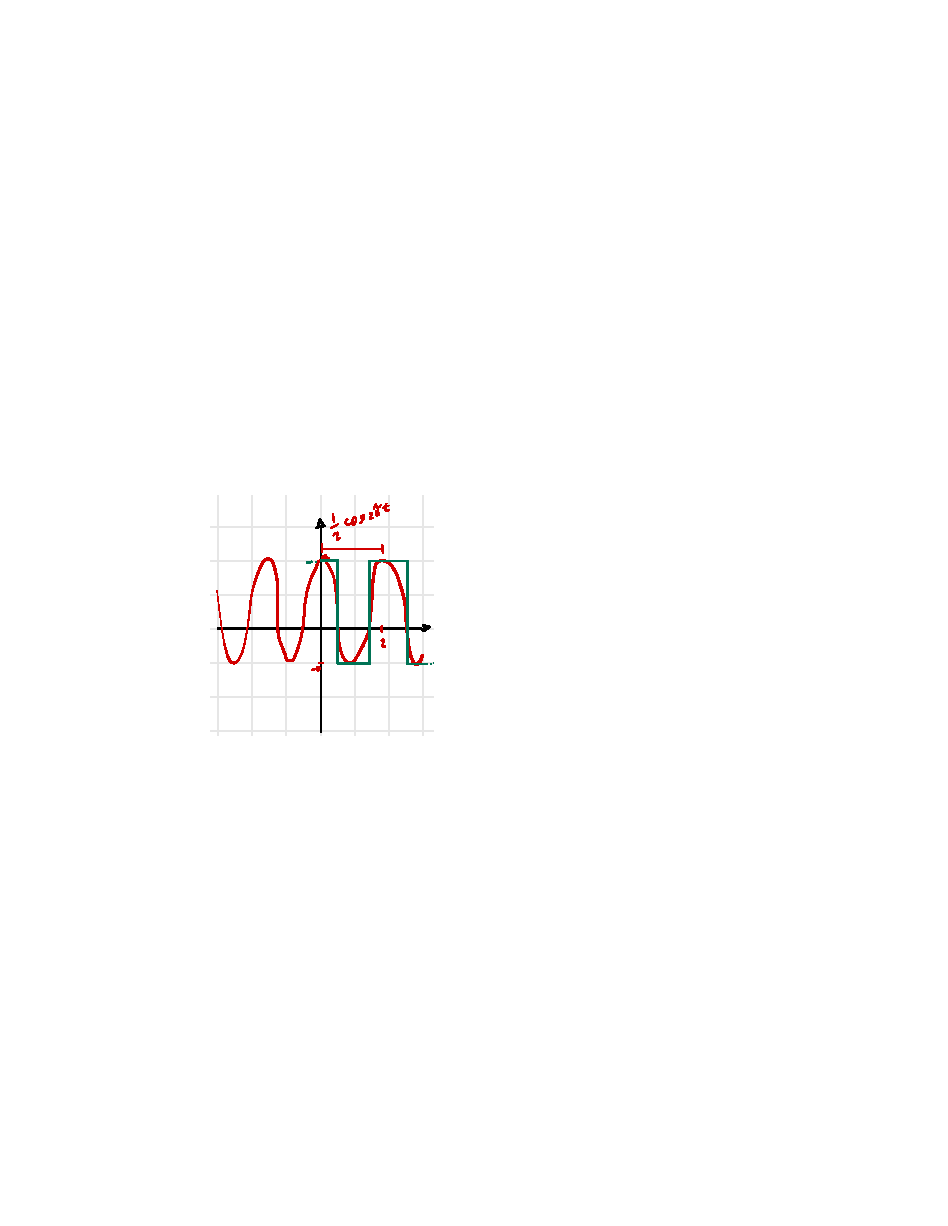
\includegraphics[width=0.4\textwidth]{img/ex_exam/sng_func_2-Mod2.pdf}
		\caption{Funzione coseno $\cos\left(2\pi\right)$ moltiplicata per $\dfrac{1}{T_0}=\dfrac{1}{2}$.}\label{ex2_grafico}
	\end{figure}
	\noindent
	\textcolor{Green4}{\textbf{\emph{Risoluzione II.}}}
	
	\noindent
	Si conclude l'esercizio calcolando l'energia o la potenza del segnale. Per farlo, dato che non è definito in un intervallo ma continua all'infinito, si calcolano i rispettivi integrali in un intervallo arbitrario $n$ e poi lo si estende all'infinito:
	
	\begin{gather*}
		E_{f} = \int_{-\infty}^{\infty} f^{2}(t) \:\mathrm{d}t = \lim_{n\rightarrow\infty} \int_{-n\cdot\frac{T_0}{2}}^{n\cdot\frac{T_0}{2}} f^{2}(t) \:\mathrm{d}t = \lim_{n\rightarrow\infty} n\cdot\int_{-\frac{T_0}{2}}^{\frac{T_0}{2}} f^{2} (t) \:\mathrm{d}t = \infty \\
		P_{f} = \lim_{T\rightarrow\infty} \dfrac{1}{T} \int_{-\frac{T}{2}}^{\frac{T}{2}} f^{2}(t) \:\mathrm{d}t = \lim_{n\rightarrow\infty} \dfrac{1}{nT_{0}} \int_{-n\frac{T_{0}}{2}}^{n\frac{T_{0}}{2}} f^{2}(t)\:\mathrm{d}t = 
		\cancel{\lim_{n\rightarrow\infty}} \dfrac{1}{\cancel{n}T_{0}} \cdot \cancel{n} \cdot \int_{-\frac{T_{0}}{2}}^{\frac{T_{0}}{2}} f^{2}(t)\:\mathrm{d}t = \\
		= \dfrac{1}{T_{0}} \cdot T_{0} = \dfrac{1}{2} \cdot 2 = 1 \longrightarrow \ne 0
	\end{gather*}

	\noindent
	È evidente che il segnale è di potenza. Come si evince dalla figura~\ref{ex2_grafico}, i tratti di colore verde indicano il rettangolo formato dal segnale. Calcolando l'area del rettangolo, si ottiene esattamente il valore di $T_{0}$. Infatti, la base del rettangolo (verticale) è $2$, mentre l'altezza (orizzontale) è $1$.
	
	\newpage
	
	\subsubsection{Cross-Correlazione Normalizzata}
	
	Ha l'\textbf{obbiettivo} di trattare segnali con range di valori diversi e consente di eseguire \textbf{confronti uno-a-molti} (\emph{one-to-many}):
	
	\begin{equation*}
		f_{1} \bar{\otimes} f_{2}\left(t\right) = \dfrac{\displaystyle \int_{-\infty}^{+\infty} \tilde{f_{1}}\left(\tau\right) f_{2}\left(\tau - t\right) \: \mathrm{d}\tau}{\displaystyle \sqrt{E_{f_{1}} E_{f_{2}}}}
	\end{equation*}
	
	\noindent
	In cui $E_{f}$ indica l'\textbf{energia} del segnale $f$. Ci sono due caratteristiche importanti:
	
	\begin{itemize}
		\item $f_{1} \bar{\otimes} f_{2}\left(t\right) \in \left[-1, 1\right]$
		
		\item $\left|f_{1} \bar{\otimes} f_{2}\left(t\right)\right| = 1 \iff f_{1}\left(\tau\right) = \alpha f_{2} \left(\tau - t\right)$
	\end{itemize}
	
	\noindent
	Inoltre, si parla di \textbf{autocorrelazione} (normalizzata e non) quando $f_{1} = f_{2}$. Utile per i segnali stocastici.\newline
	
	\noindent
	Nel \textbf{\emph{caso di segnali discreti}}, dati $x_{1}\left(k\right), x_{2}\left(k\right)$:
	
	\begin{equation*}
		x_{1} \otimes x_{2}\left(n\right) = \sum_{k = -\infty}^{+\infty} \tilde{x_{1}}\left(k\right) x_{2} \left(k - n\right) \hspace{1em} k \in \mathbb{Z}
	\end{equation*}

	\noindent
	Sotto l'ipotesi di convergenza della serie, cioè la serie deve convergere.\newline
	
	\noindent
	Nel caso in cui $x_{1}\left(k\right)$ e $x_{2}\left(k\right)$ sono limitati di lunghezza M ed N rispettivamente, allora la \textbf{cross correlazione è di lunghezza} $M+N-1$.
	
	\newpage
	
	\noindent
	\textcolor{Green4}{\textbf{Cross-Correlazione 1D}}\newline
	
	\noindent
	Data la definizione:
	
	\begin{equation*}
		x_{1} \otimes x_{2}\left(n\right) = \sum_{k = -\infty}^{+\infty} x_{1}\left(k\right) x_{2}\left(k - n\right)
	\end{equation*}
	
	\noindent
	Esistono diverse casistiche:
	
	\begin{itemize}
		\item $n = 0$ si confronta tra $x_{1}$ e $x_{2}$ nei loro domini temporali originali.
		
		\item $n > 0$ sposto $x_{2}$ a destra poiché c'è l'anticipo di $x_{2}$
		
		\item $n < 0$ sposto $x_{2}$ a sinistra poiché c'è ritardo di $x_{2}$
	\end{itemize}

	\begin{figure}[!htp]
		\centering
		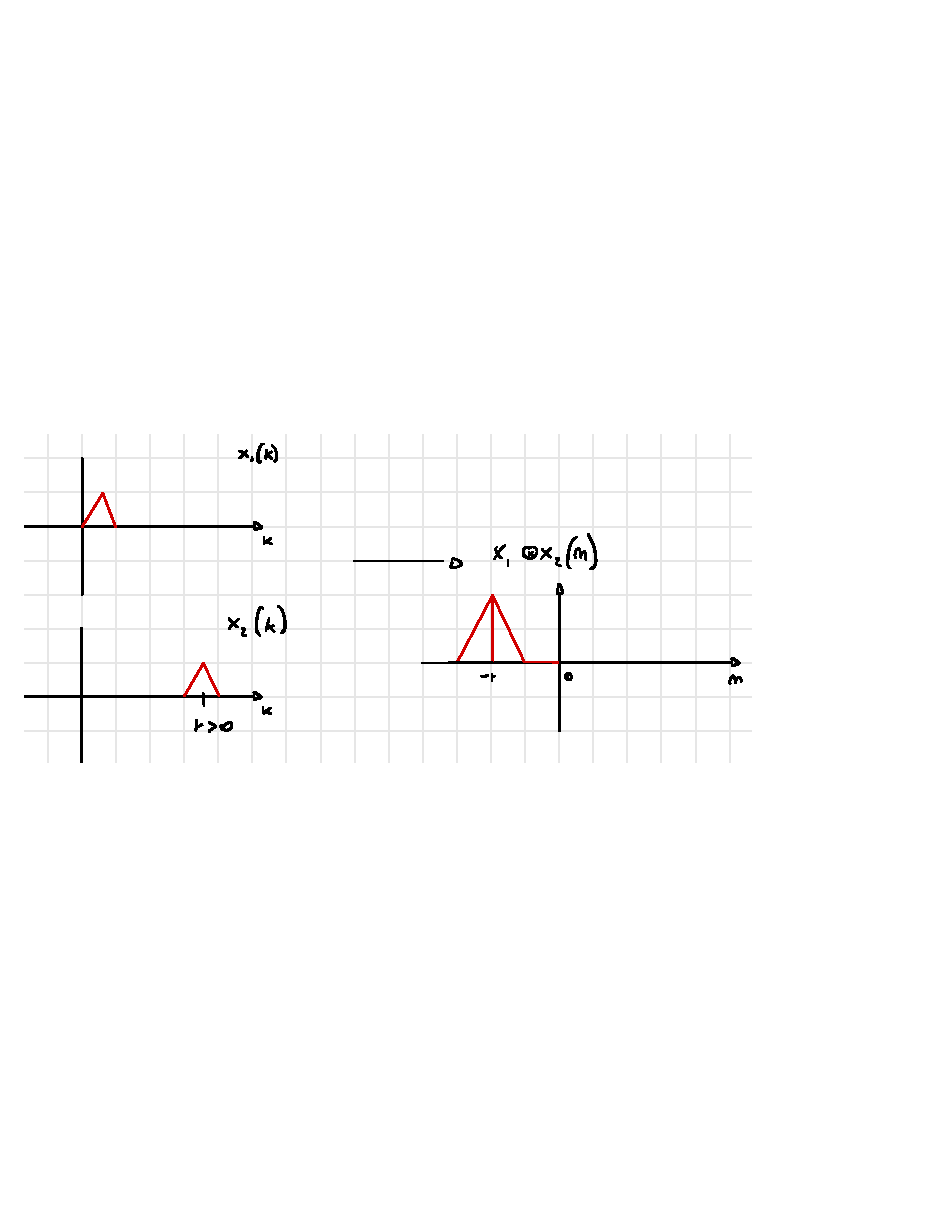
\includegraphics[width=0.9\textwidth]{img/ex_exam/eg_cross-correlazione-1D.pdf}
		\caption{Esempio di cross-correlazione normalizzata 1D.}
	\end{figure}

	\noindent
	Il triangolo $x_{2}$ va verso sinistra e il lasso di tempo che $x_{2}$ non combacia con $x_{1}$, viene rappresentato come una linea orizzontale sull'asse delle $n$ nel piano cartesiano di destra.
	
	\newpage
	
	\noindent
	\textcolor{Green4}{\textbf{Cross-Correlazione 2D}}\newline
	
	\noindent
	Data la definizione:
	
	\begin{equation*}
		x_{1} \otimes x_{2}\left(m, n\right) = \sum_{u = -\infty}^{+\infty} \sum_{v = -\infty}^{+\infty} x_{1}\left(u, v\right) x_{2}\left(u - m, v - n\right) \hspace{1em} u,v,m,n \in \mathbb{Z}
	\end{equation*}
	
	\noindent
	Nel 2D $x_{1}$ e $x_{2}$ possono essere pensate come \textbf{immagini infinite}.\newline
	
	\noindent
	Di solito $x_{1}$ e $x_{2}$ sono \textbf{immagini finite} (segnali digitali ad intervallo limitato), e gli estremi di sommatoria sono quindi finiti.\newline
	
	\noindent
	Il primo segnale $x_{1}$ viene chiamato \textbf{\emph{template}}, o \textbf{\emph{matrice kernel}}, mentre $x_{2}$ genericamente \textbf{immagine} (di solito, la matrice kernel $x_{1}$ ha una dimensionalità minore di quella dell'immagine).\newline
	
	\noindent
	Nel caso $x_{1} = x_{2}$ si ha \textbf{autocorrelazione 2D}.\newline
	
	\noindent
	\textcolor{Green4}{\textbf{Cross-Correlazione normalizzata 2D}}\newline
	
	\noindent
	Si definisce come:
	
	\begin{equation*}
		x_{1} \otimes x_{2}\left(m,n\right) = \dfrac
		{\sum_{u = -\infty}^{+\infty} \sum_{v = -\infty}^{+\infty} \left[x_{1}\left(u, v\right)\right]\left[x_{2}\left(u-m, v-n\right)\right]}
		{\sqrt{\sum_{u = -\infty}^{+\infty} \sum_{v = -\infty}^{+\infty} \left[x_{1}\left(u,v\right)\right]^{2} {\sum_{u = -\infty}^{+\infty} \sum_{v = -\infty}^{+\infty} \left[x_{2}\left(u,v\right)\right]^{2}}}}
	\end{equation*}

	\noindent
	In altre parole, fissato il punto di applicazione $n, m$, si sottrae la media ad ogni punto nell'interno di applicazione dalla matrice kernel. Successivamente, si divide per il prodotto della varianza dei due segnali, estraendo a radice alla fine.
	
	\begin{figure}[!htp]
		\centering
		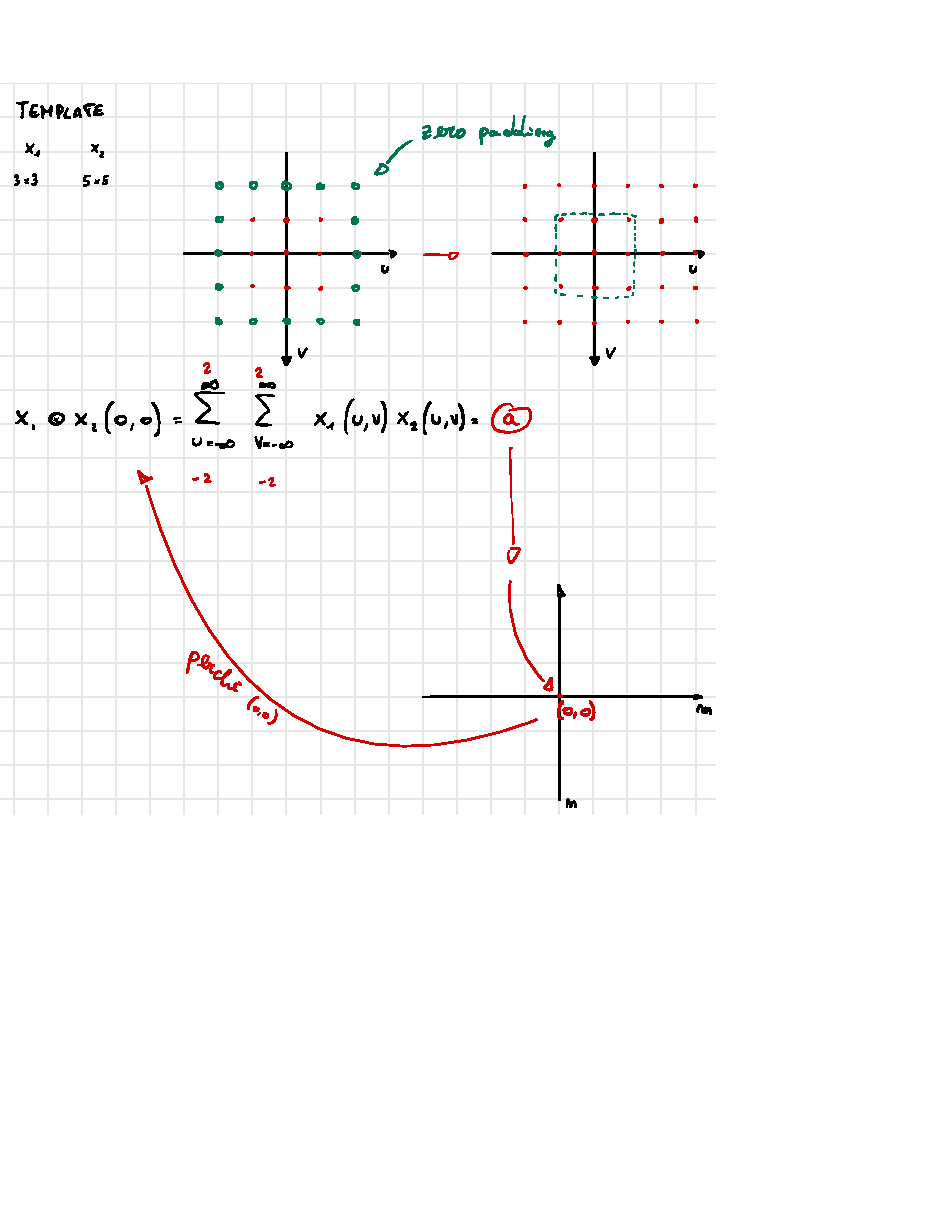
\includegraphics[width=1\textwidth]{img/ex_exam/eg_cross-correlazione-2D.pdf}
		\caption{Esempio di Cross-Correlazione normalizzata 2D.}
	\end{figure}

	\newpage
	
	\noindent
	\textcolor{Red3}{\textbf{Esercizio Cross-Correlazione 2D}}\newline
	
	\noindent
	Dati le due immagini $x_{1}$ di dimensione $5 \times 5$ e $x_{2}$ di dimensione $3 \times 3$, si calcola la cross-correlazione 2D. Quindi, si effettua la rappresentazione grafica.
	
	\begin{figure}[!htp]
		\centering
		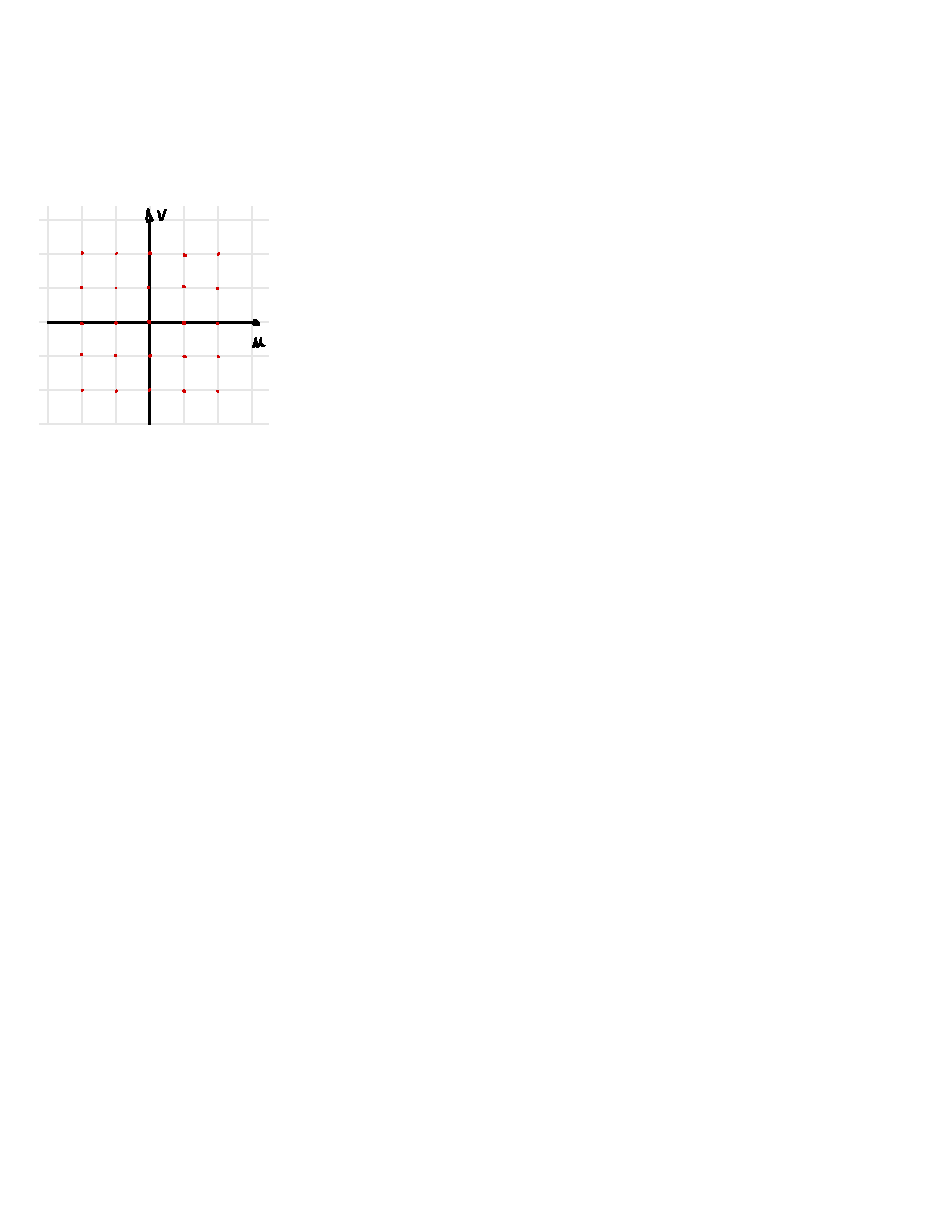
\includegraphics[width=0.5\textwidth]{img/cross-correlazione-2D_ex1.pdf}
		\caption{Piano cartesiano di $x_{2}$ di dimensione $5 \times 5$.}
		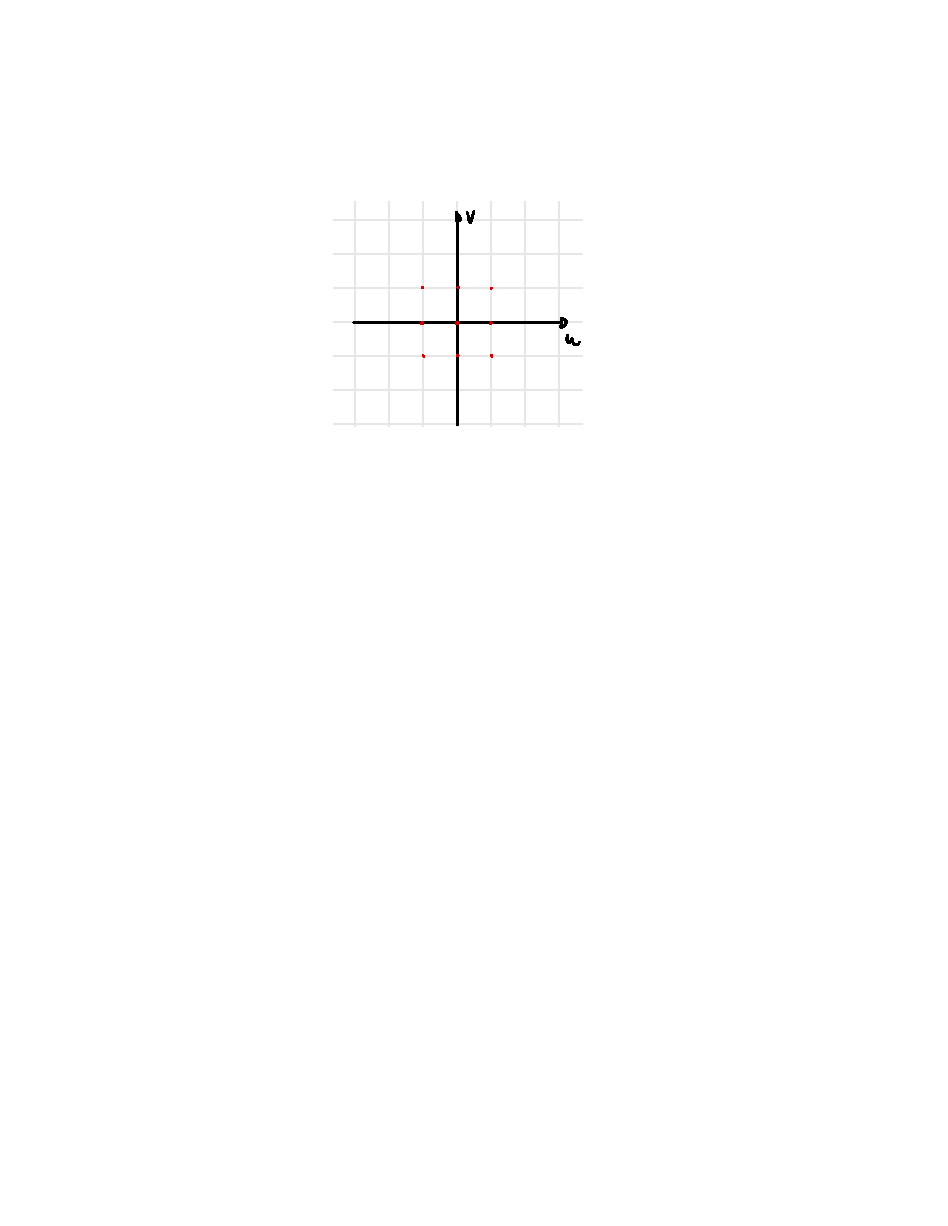
\includegraphics[width=0.5\textwidth]{img/cross-correlazione-2D_ex1_1.pdf}
		\caption{Piano cartesiano di $x_{1}$ di dimensione $3 \times 3$.}
	\end{figure}

	\noindent
	E vengono fornite dall'esercizio le due matrici:
	
	\begin{equation*}
		x_{2} =
		\begin{bmatrix}
			1 & 0 & 0 & 0 & 0 \\
			0 & 1 & 0 & 0 & 0 \\
			0 & 0 & 1 & 0 & 0 \\
			0 & 1 & 1 & 0 & 1 \\
			0 & 0 & 0 & 1 & 0 \\
		\end{bmatrix}
		\hspace{2em}
		x_{1} =
		\begin{bmatrix}
			1 & 0 & 0 \\
			0 & 1 & 0 \\
			0 & 0 & 1 \\
		\end{bmatrix}		
	\end{equation*}

	\noindent
	Esse indicano i valori nei punti corrispondenti. L'\textbf{obbiettivo dell'esercizio} è trovare:
	
	\begin{itemize}
		\item L'argomento massimo della cross-correlazione ($\arg \max x_{1} \otimes x_{2}\left(m,n\right)$);
		
		\item Il massimo della cross-correlazione ($\max x_{1} \otimes x_{2} \left(m,n\right)$).
	\end{itemize}

	\noindent
	L'argomento massimo è con i valori $m = 1$ e $n = -1$ poiché così facendo la diagonale incontra tutti i valori positivi e che formano il massimo. Infatti, prendendo in considerazione la matrice $x_{2}\:5 \times 5$ e osservando l'operazione di cross-correlazione 2D:
	
	\begin{gather*}
		\sum_{u} \sum_{v} x_{1} \left(u,v\right) \cdot x_{2}\left(u - m, v - n\right) \\
		\xrightarrow{\text{sostituzione termini noti } (m, n)} \sum_{u} \sum_{v} x_{1} \left(u,v\right) \cdot x_{2}\left(u - 1, v - \left(-1\right)\right)
	\end{gather*}

	\noindent
	Risulta evidente come si debba spostare a destra, rispetto l'origine, la matrice $x_{2}$ di un solo valore\footnote{Shift a destra poiché $u-1$ nell'equazione rappresenta un ritardo.} e sotto, rispetto sempre l'origine, di un valore negativo\footnote{Spostamento sotto l'asse delle ascisse poiché è un valore positivo $v+1$.}. Così facendo, la diagonale della matrice $x_{2}$ corrisponderà esattamente a tutti i valori $1$ della matrice $x_{1}$.

	\newpage
	
	\subsubsection{Convoluzione}
	
	La \textbf{convoluzione} è un parente stretto della cross-correlazione, ma è leggermente diverso. È definito nel seguente modo:
	
	\begin{equation*}
		f_{1} * f_{2}\left(t\right) = \int_{-\infty}^{+\infty} f_{1}\left(\tau\right) f_{2}\left(t - \tau\right) \mathrm{d}\tau
	\end{equation*}

	\noindent
	Con $t in \mathbb{R}$. Si ricordi che se i \textbf{segnali non sono né di energia né di potenza, l'integrale \underline{converge}}.\newline
	
	\noindent
	Nel caso in cui i \textbf{segnali} siano \textbf{discreti}, dati $x_{1}\left(n\right)$, $x_{1}\left(n\right)$:
	
	\begin{equation*}
		x_{1} * x_{2} \left(n\right) = \sum_{k = -\infty}^{+\infty} x_{1}\left(k\right) x_{2}\left(n - k\right)
	\end{equation*}

	\noindent
	Con $k \in \mathbb{Z}$.
	
	\noindent
	Nel caso in cui $x_{1} \left(n\right)$ e $x_{2} \left(n\right)$ sono limitati di lunghezza $M$ ed $N$ rispettivamente, allora la \textbf{convoluzione è di lunghezza} $M+N-1$.\newline
	
	\noindent
	\textcolor{Green4}{\textbf{Convoluzione 2D}}\newline
	
	\noindent
	Nel caso delle immagini, quindi del 2D, $x_{1}$ ed $x_{2}$ sono solitamente \textbf{segnali digitali ad intervallo limitato}, e la convoluzione diventa dunque:
	
	\begin{equation*}
		x_{1} * x_{2}\left(m,n\right) = \sum_{u = -\infty}^{+\infty} \sum_{v = -\infty}^{+\infty} x_{1} \left(u,v\right) x_{2}\left(m - u, n - v\right) \hspace{2em} u,v,m,n\in\mathbb{Z}
	\end{equation*}

	\noindent
	Solitamente il primo segnale $x_{1}$ viene chiamato \textbf{\underline{filtro}}, o \textbf{\underline{matrice kernel}}, mentre $x_{2}$ genericamente \textbf{\underline{immagine}} (solitamente la matrice kernel ha una dimensione inferiore di quella dell'immagine).
	
	\newpage
	
	\section{Analisi di Fourier}
	
	\subsection{Serie di Fourier}\label{serie di fourier}
	
	Una funzione, chiamata \textbf{\underline{funzione di sintesi}}, $f: \mathbb{R} \rightarrow \mathbb{R}$ di variabile continua $t$, periodica di periodo $T$, si esprime come:
	
	\begin{equation*}
		f(t) = \sum_{n = -\infty}^{+\infty} c_{n} \underbrace{e^{j \frac{2\pi n}{T}t}}_{\text{fasore}} \hspace{2em} n\in\mathbb{Z}
	\end{equation*}

	\noindent
	Dove $c_{n}$ è un numero complesso. Invece, una \textbf{\underline{funzione di analisi}} è espressa come:
	
	\begin{equation*}
		c_{n} \in \mathbb{C} = \dfrac{1}{T} \int_{-\frac{T}{2}}^{+\frac{T}{2}} f\left(t\right) \underbrace{e^{-j \frac{2\pi n}{T}t}}_{\text{fasore}} \mathrm{d}t \hspace{2em} n \in \mathbb{Z}
	\end{equation*}

	\noindent
	\textbf{N.B.} si ricorda che $e^{j \frac{2\pi n}{T}t}$ è un \textbf{fasore rotante} di velocità angolare $\dfrac{2\pi n}{T} t$.\newline
	La \textbf{\underline{funzione di sintesi}} quindi non è altro che una somma di infiniti termini. Ciascuno è composto dalla moltiplicazione tra un numero complesso ed un fasore, il quale \emph{produce un altro fasore}. Esprimendo $c_{n}$ come numero complesso in forma polare:
	
	\begin{equation*}
		c_{n} e^{j \frac{2 \pi n}{T} t} = |c_{n}| e^{j \theta_{n}} e^{j \frac{2 \pi n}{T} t} = |c_{n}| e^{j \left(\frac{2 \pi n}{T} t + \theta_{n}\right)}
	\end{equation*}

	\noindent
	Si può notare come questa conversione corrisponda ad \textbf{estendere} il fasore $e^{j\frac{2 \pi n}{T} t}$ ad una lunghezza $|c_{n}|$ facendolo partire con un \textbf{angolo di partenza} uguale a $\theta_{n}$ (chiamato \textbf{\underline{angolo di fase}}).\newline
	
	\noindent
	\textbf{\underline{Altra osservazione:}} se $c_{n}$ appartiene all'insieme $\mathbb{R}$, significa che $\theta_{n}$ non compare. Questo comporta un cambiamento nella lunghezza dell'$n$-esimo fasore pari a $|c_{n}|$:
	
	\begin{equation*}
		c_{n} = |c_{n}| \cancel{e^{j \theta_{n}}}
	\end{equation*}

	\newpage
	
	\noindent
	\textcolor{Green4}{\textbf{\underline{Esempio 1}}}\newline
	
	\noindent
	Il primo esempio di serie di Fourier si applica per il segnale trigonometrico:
	
	\begin{equation*}
		f\left(t\right) = \cos\left(2 \pi t\right) \hspace{2em} \text{con } T = 1
	\end{equation*}

	\noindent
	Applicando la \textbf{funzione di analisi} e saltando i passaggi perché complessi, si ottengono i seguenti valori:
	
	\begin{equation*}
		c_{-1} = \dfrac{1}{2} \hspace{3em}
		c_{0} = 0 \hspace{3em}
		c_{1} = \dfrac{1}{2} \hspace{3em}
		c_{i \le -2, i \ge 2} = 0
	\end{equation*}

	\noindent
	E sostituendo nella \textbf{funzione di sintesi}:
	
	\begin{equation*}
		\cos\left(2 \pi t\right) = \dfrac{1}{2} e^{-j 2 \pi t} + \dfrac{1}{2} e^{j 2 \pi t} = \dfrac{e^{j 2 \pi t} + e^{-j 2 \pi t}}{2}
	\end{equation*}

	\noindent
	Ci sono \textbf{tre osservazioni} da fare:
	
	\begin{enumerate}[label=\Roman*.]
		\item $\dfrac{2\pi}{T} = f_{0}$;
		
		\item $c_{n} = |c_{n}| e^{j\theta_{n}}$;
		
		\item In questo caso, $c_{n} \in \mathbb{R}$ quindi l'angolo di fase non è presente.
	\end{enumerate}

	\noindent
	\textbf{Le parti} dell'equazione sono le seguenti:
	
	\begin{equation*}
		\cos{\left(2 \pi t\right)} = \dfrac{1}{2} e^{-j 2 \pi t} + \dfrac{1}{2} e^{j 2 \pi t}
	\end{equation*}

	\begin{itemize}[label=\ding{43}]
		\item $\cos{\left(2 \pi t\right)} \rightarrow$ La funzione trigonometrica da studiare
		
		\item $\dfrac{1}{2} e^{-j 2 \pi t} \rightarrow$ Fasore di modulo $0.5$ e velocità angolare $-2\pi t$
		
		\item $\dfrac{1}{2} e^{j 2 \pi t} \rightarrow$ Fasore di modulo $0.5$ e velocità angolare $2\pi t$
	\end{itemize}

	\begin{figure}[!htp]
		\centering
		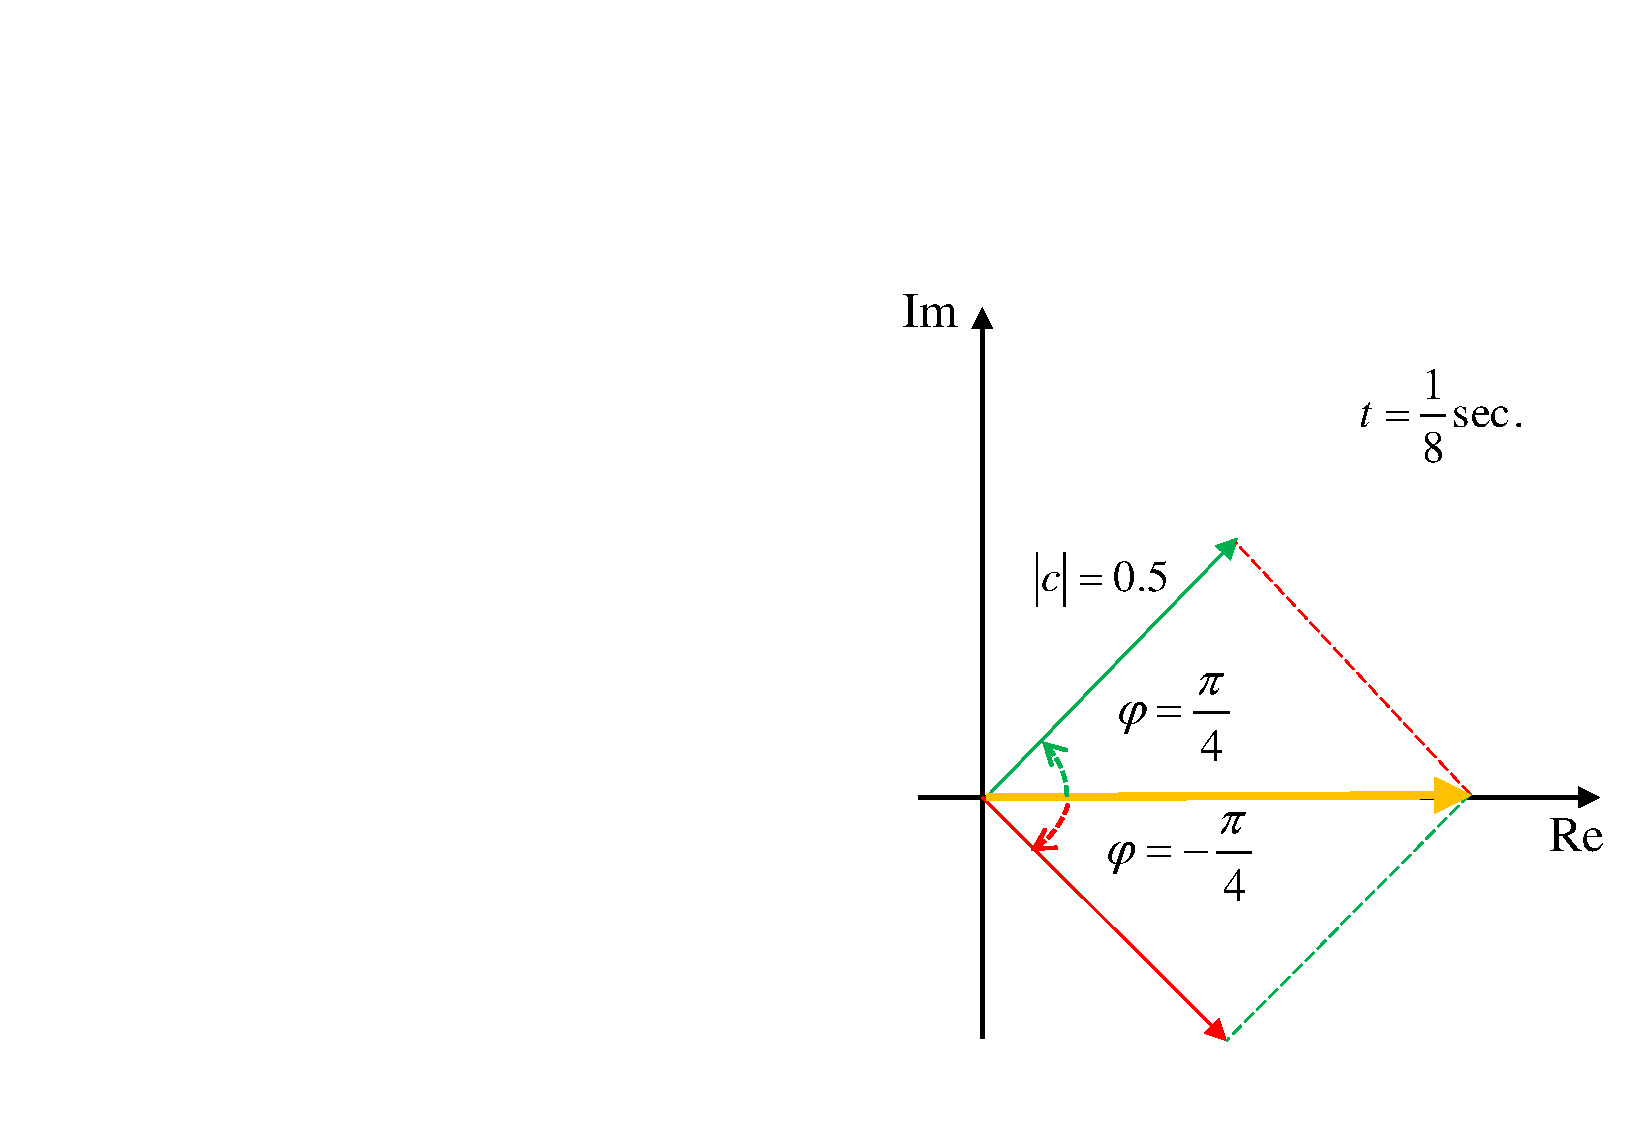
\includegraphics[width=0.5\textwidth]{img/fourier_eg1.pdf}
		\caption{Grafico rappresentante i due fasori. La freccia verde rappresenta il valore assunto da $\cos{\left(2\pi t\right)}$ per $t = \dfrac{1}{8}$.}
	\end{figure}

	\noindent
	I coefficienti $c_{n = -1}$ e $c_{n = 1}$ sono relativi ai \textbf{\underline{moduli o ampiezze}} \textbf{dei fasori} complessi di frequenza $f_{0} \cdot n$ con $n = -1,1$ e ricordando che:
	
	\begin{equation*}
		\exp\left(j \left(\dfrac{2 \pi n}{T} t\right)\right) = \exp\left(j \left(f_{0} n t\right)\right)
	\end{equation*}

	\noindent
	Che si possono annotare con le variabili $f_{-1}$ e $f_{1}$ per $f_{0} \cdot n$ con $n = -1, 1$ e analogamente per gli altri $n \in \mathbb{Z}$.\newline
	
	\noindent
	Inoltre, è possibile disegnare lo \textbf{\underline{spettro di ampiezza}} che \textbf{mostra i moduli dei fasori costruiti con la trasformata di Fourier}, in particolare la funzione di sintesi.
	
	\begin{figure}[!htp]
		\centering
		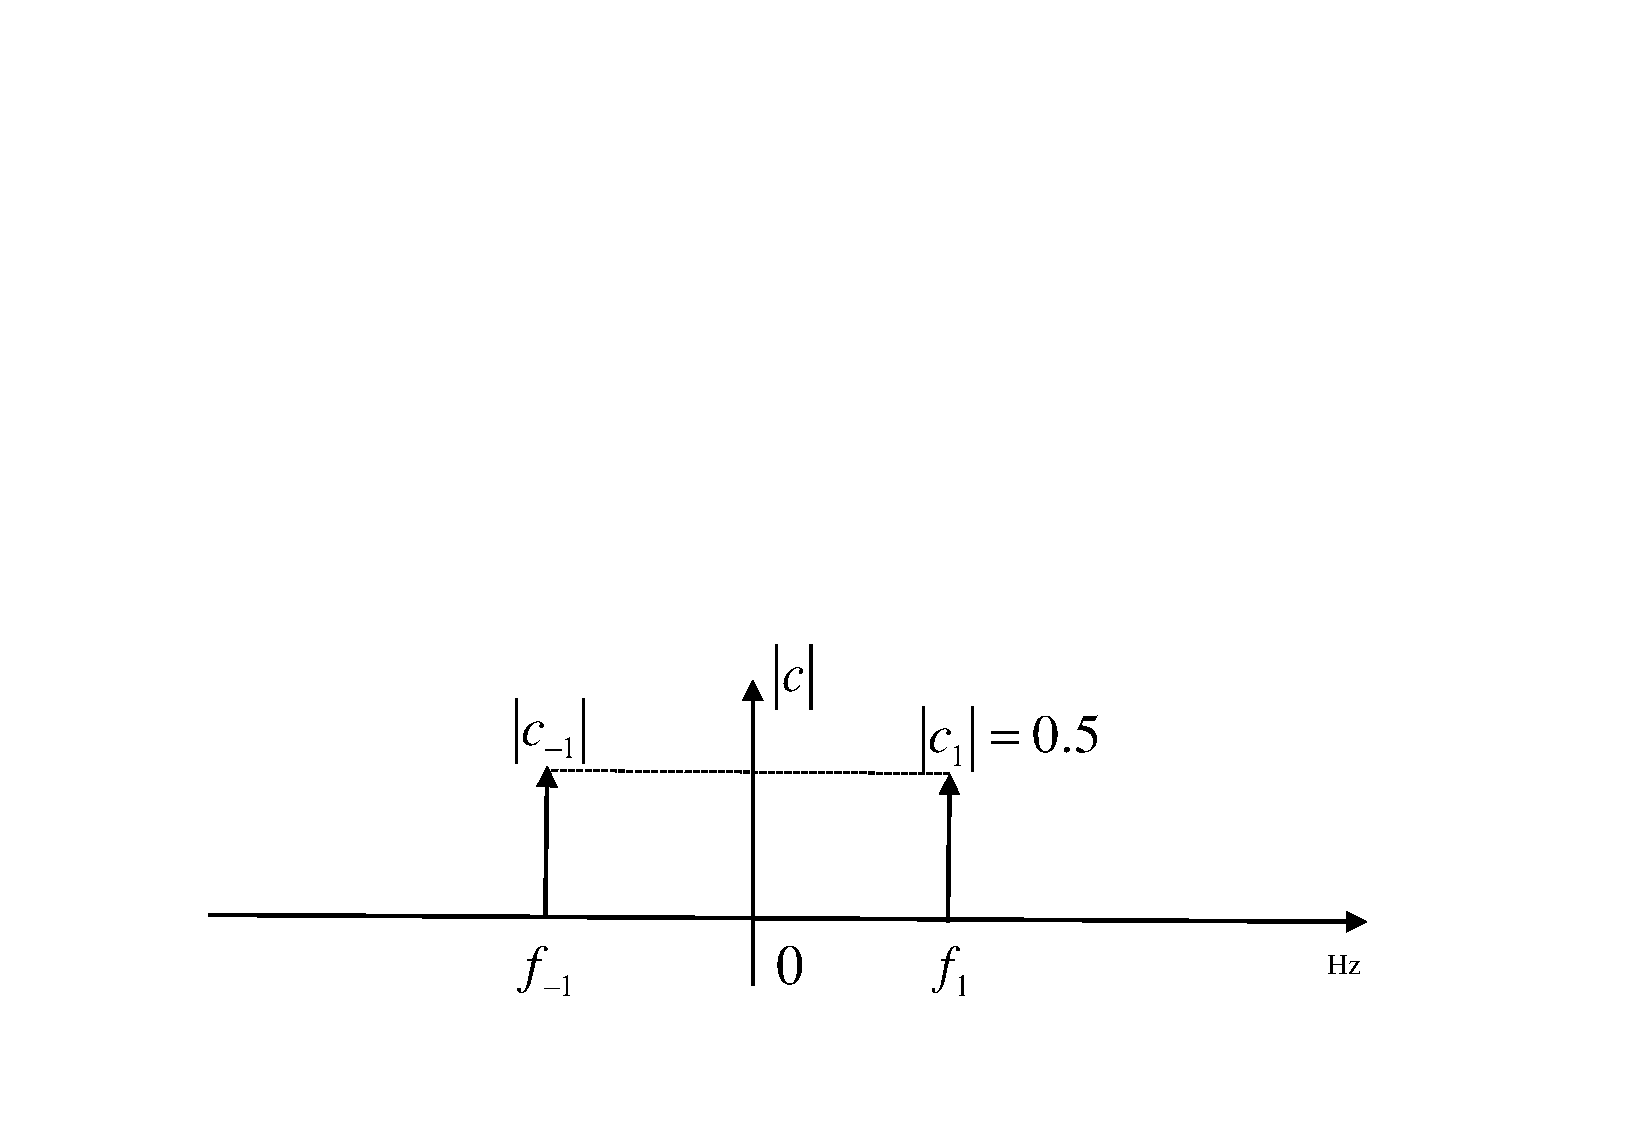
\includegraphics[width=0.9\textwidth]{img/fourier_spettro_di_ampiezza.pdf}
		\caption{Grafico che rappresenta lo spettro di ampiezza.}
	\end{figure}

	\newpage
	
	\noindent
	\textcolor{Green4}{\textbf{\underline{Esempio 2}}}\newline
	
	\noindent
	Il secondo esempio di serie di Fourier è il segnale trigonometrico:
	
	\begin{equation*}
		f\left(t\right) = \sin\left(2 \pi t\right) \hspace{2em} \text{con } T = 1
	\end{equation*}

	\noindent
	Applicando la \textbf{funzione di analisi} e saltando i passaggi perché complessi, si ottengono i seguenti valori:
	
	\begin{equation*}
		c_{-1} = -\dfrac{1}{2j} \hspace{3em}
		c_{0} = 0 \hspace{3em}
		c_{1} = \dfrac{1}{2j} \hspace{3em}
		c_{i \le -2, i \ge 2} = 0
	\end{equation*}

	\noindent
	Dove questa volta $c_{n} \in \mathbb{C}$ ed in particolare:
	
	\begin{equation*}
		\pm \dfrac{1}{2j} = \pm \dfrac{1}{2j} \cdot \dfrac{j}{j} = \pm \dfrac{1}{2} \cdot \dfrac{j}{j^{2}} = j \cdot \mp \dfrac{1}{2}
	\end{equation*}

	\noindent
	Si passa alla forma di esponenziale complesso:
	
	\begin{gather*}
		j \cdot \dfrac{1}{2} = 0 + j \cdot \dfrac{1}{2} \\
		|c| = \sqrt{0^{2} + \left(\dfrac{1}{2}\right)^{2}} = \dfrac{1}{2} \\
		\theta = \arctan\left(\dfrac{0.5}{0}\right) \rightarrow \dfrac{\pi}{2} \\
		\dfrac{1}{2} e^{j \cdot \frac{\pi}{2}} = c_{-1}
	\end{gather*}

	\begin{figure}[!htp]
		\centering
		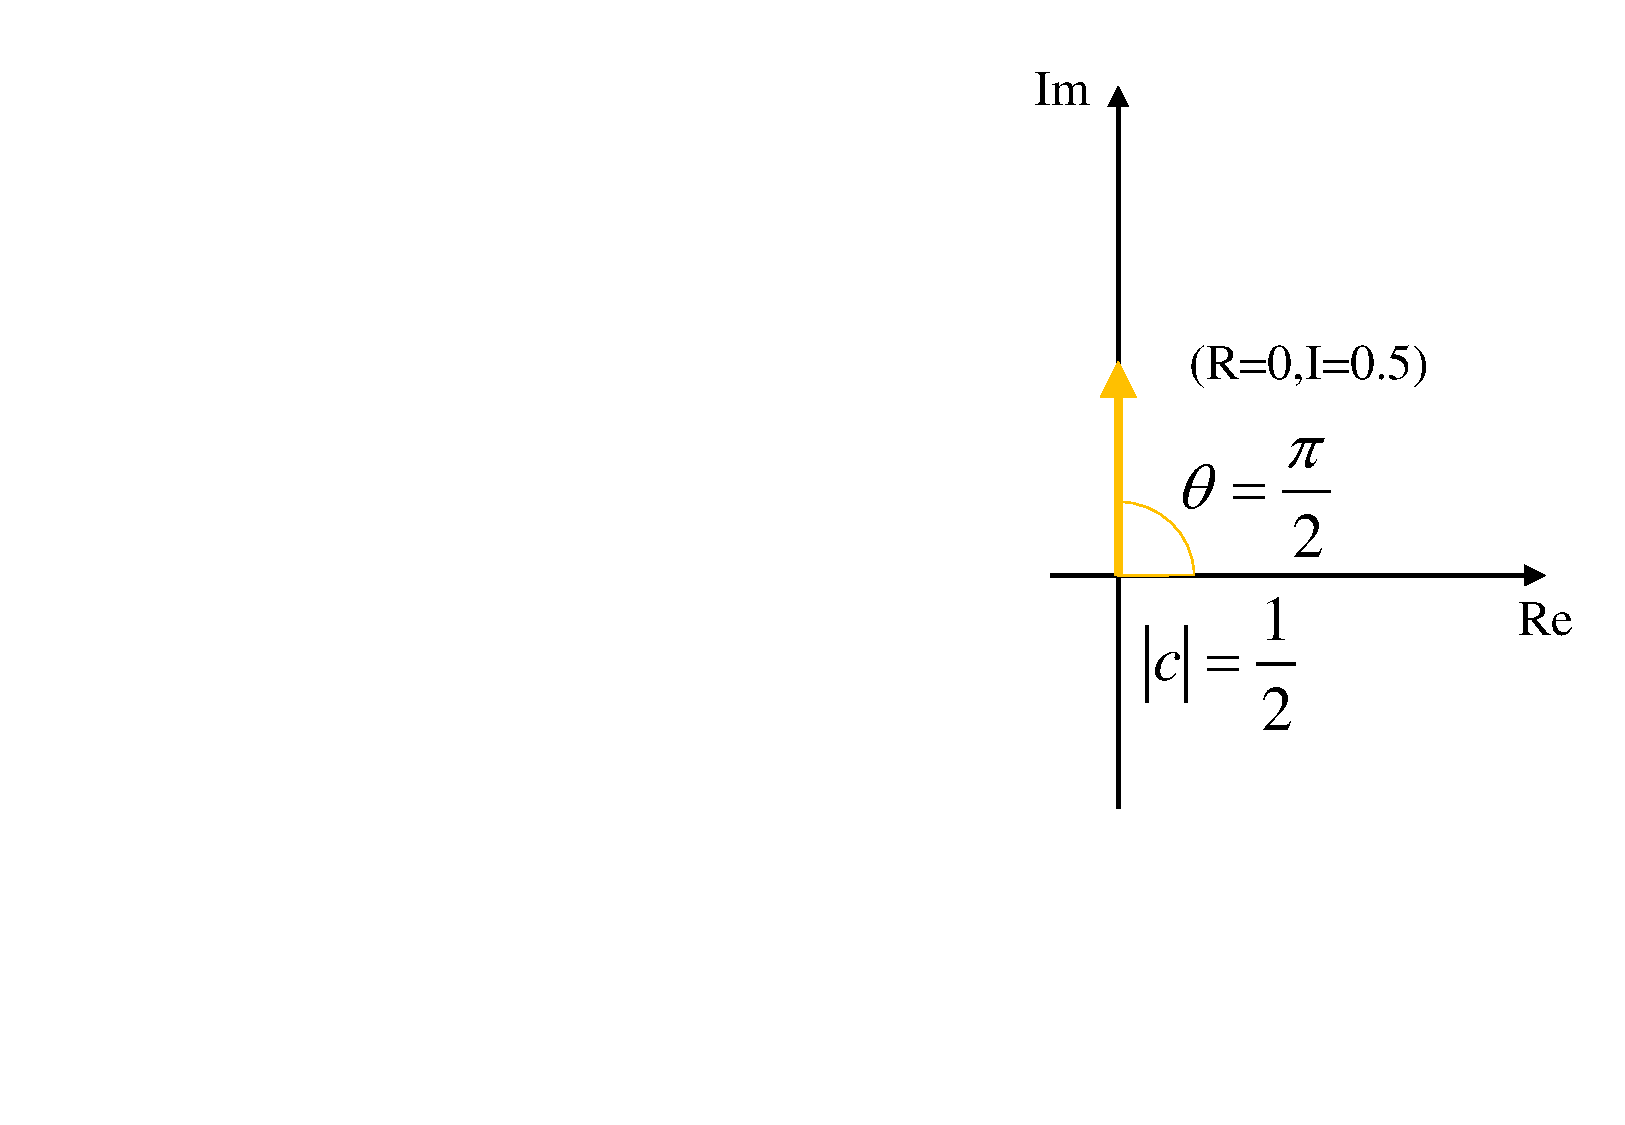
\includegraphics[width=0.3\textwidth]{img/fourier_eg2.pdf}
		\caption{Grafico di $c_{-1}$.}
	\end{figure}

	\newpage
	\noindent
	Analogamente:
	
	\begin{gather*}
		j \cdot -\dfrac{1}{2} = 0 + j \cdot \left(-\dfrac{1}{2}\right) \\
		|c| = \sqrt{0^{2} + \left(-\dfrac{1}{2}\right)^{2}} = \dfrac{1}{2} \\
		\theta = \arctan\left(-\dfrac{0.5}{0}\right) \rightarrow -\dfrac{\pi}{2} \\
		\dfrac{1}{2} e^{j \cdot \left(-\frac{\pi}{2}\right)} = c_{1}
	\end{gather*}

	\begin{figure}[!htp]
		\centering
		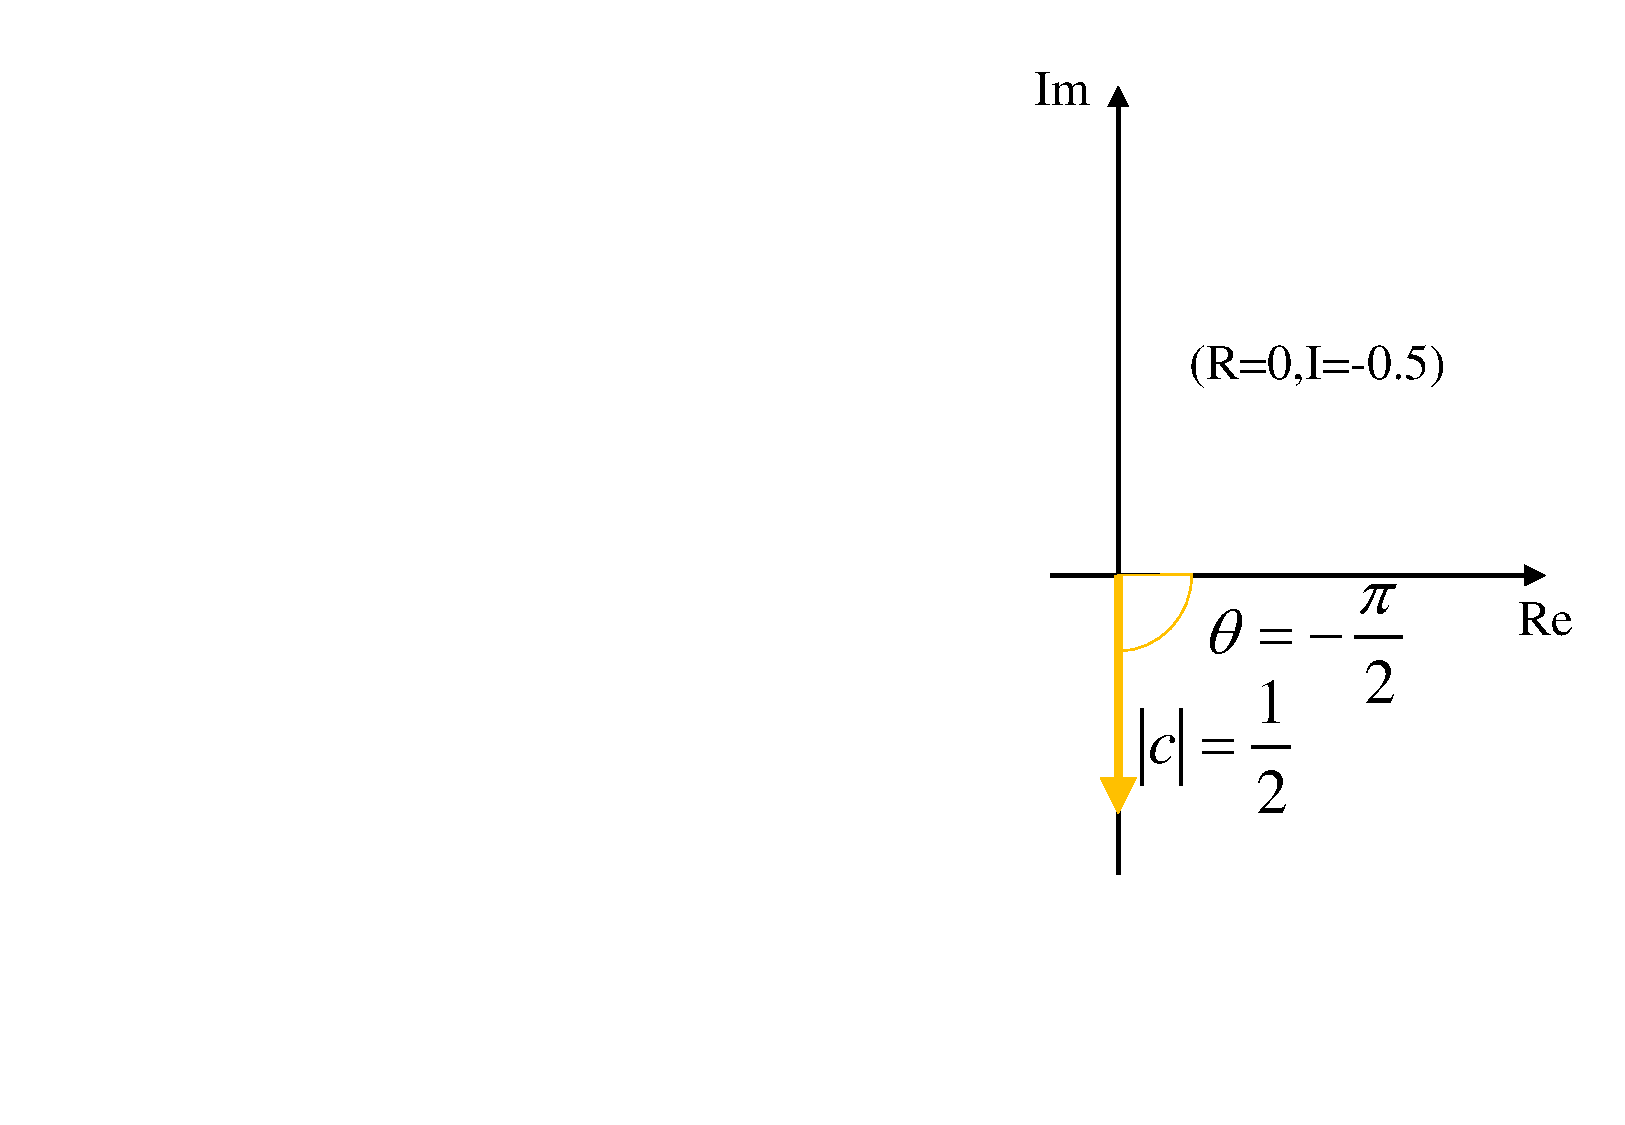
\includegraphics[width=0.3\textwidth]{img/fourier_eg2_2.pdf}
		\caption{Grafico di $c_{1}$.}
	\end{figure}

	\newpage
	\noindent
	Applicando l'\textbf{equazione di sintesi} e sostituendo i termini noti:
	
	\begin{gather*}
		\sin{\left(2 \pi t\right)} = \sum_{n = -\infty}^{+\infty} c_{n} e^{j \frac{2 \pi n}{T} t} = c_{-1} e^{j-2\pi t} + c_{1} e^{j2\pi t} \\
		\xrightarrow{\text{sostituzione dei termini noti }c_{-1}, c_{1}} = \dfrac{1}{2} e^{j \frac{\pi}{2}} e^{j \cdot \left(-2 \pi t\right)} + \dfrac{1}{2}  e^{j \frac{-\pi}{2}} e^{j 2 \pi t} \\
		\xrightarrow{\text{forma finale }} = \dfrac{1}{2} \exp{\left(j\left(-2 \pi t + \dfrac{\pi}{2}\right)\right)} + \exp{\left(j\left(2 \pi t - \dfrac{\pi}{2}\right)\right)}
	\end{gather*}

	\begin{figure}[!htp]
		\centering
		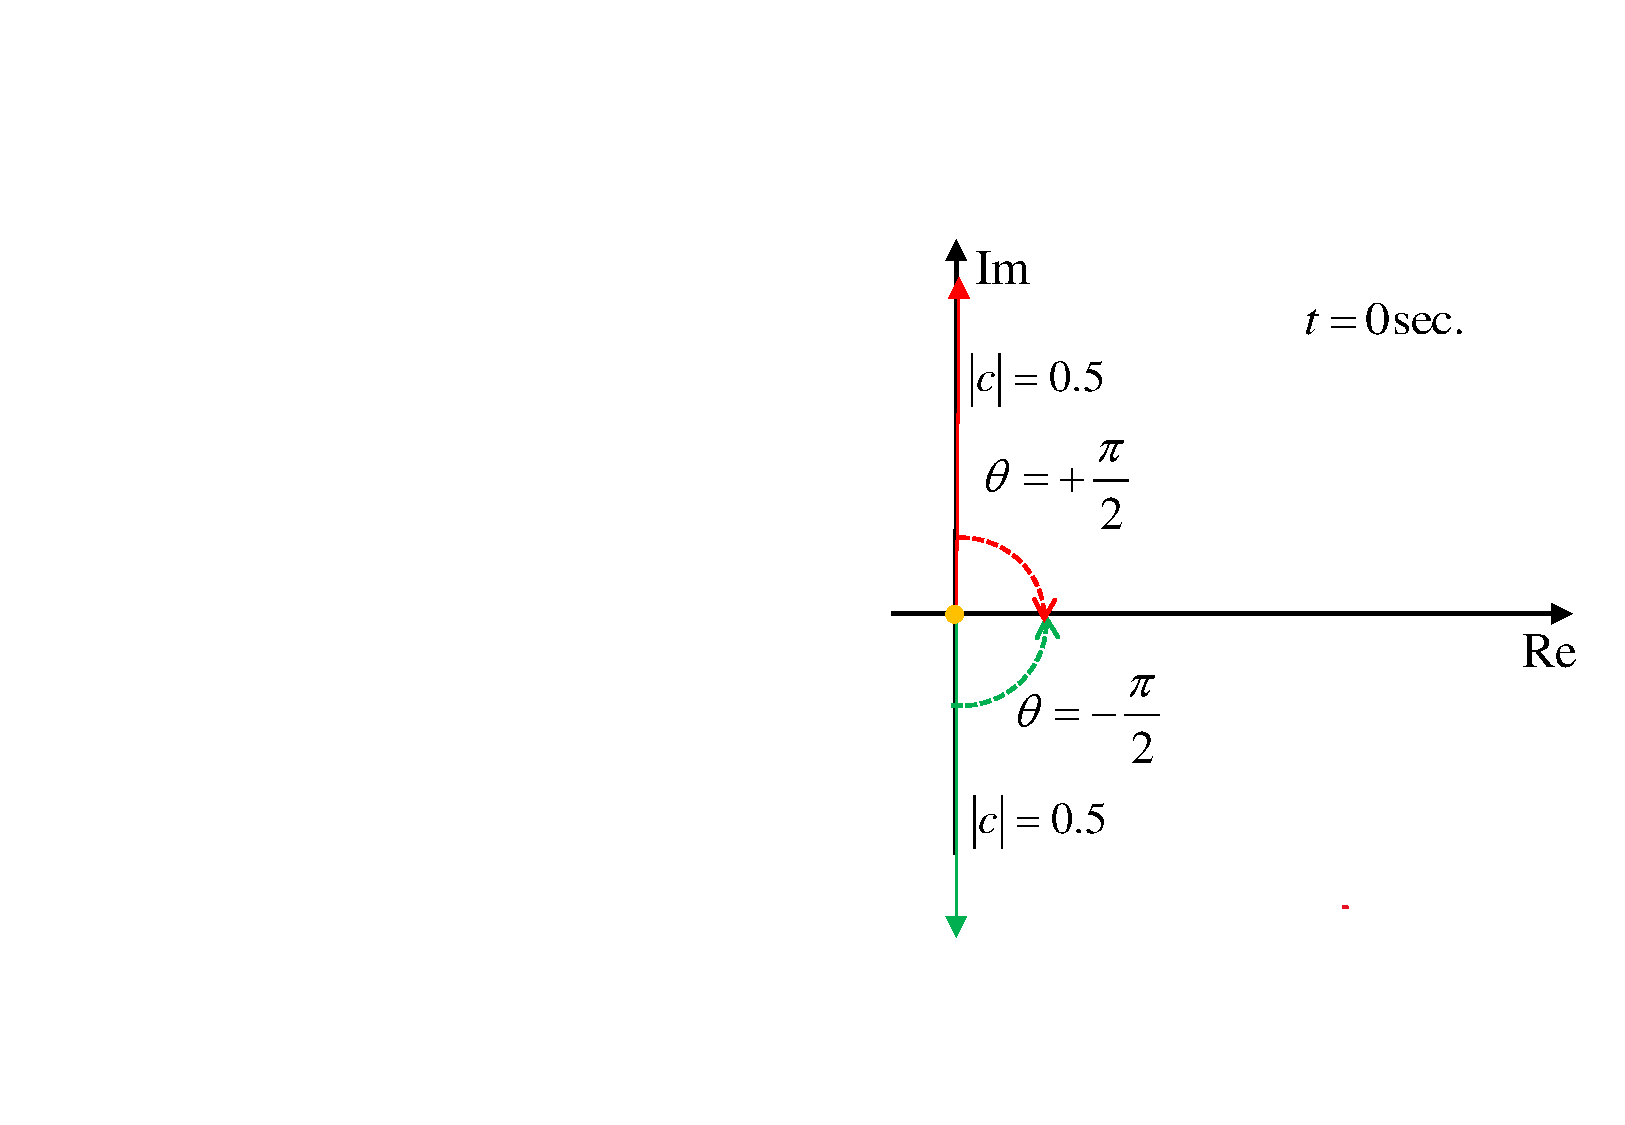
\includegraphics[width=0.5\textwidth]{img/fourier_eg2_3.pdf}
		\caption{Grafico finale.}
	\end{figure}

	\noindent
	Infine, si disegna lo \textbf{\underline{spettro di ampiezza}} e lo \textbf{\underline{spettro di fase}}, quest'ultimo è un \textbf{grafico in cui si riportano gli angoli di fase della funzione}.
	
	\begin{figure}[!htp]
		\centering
		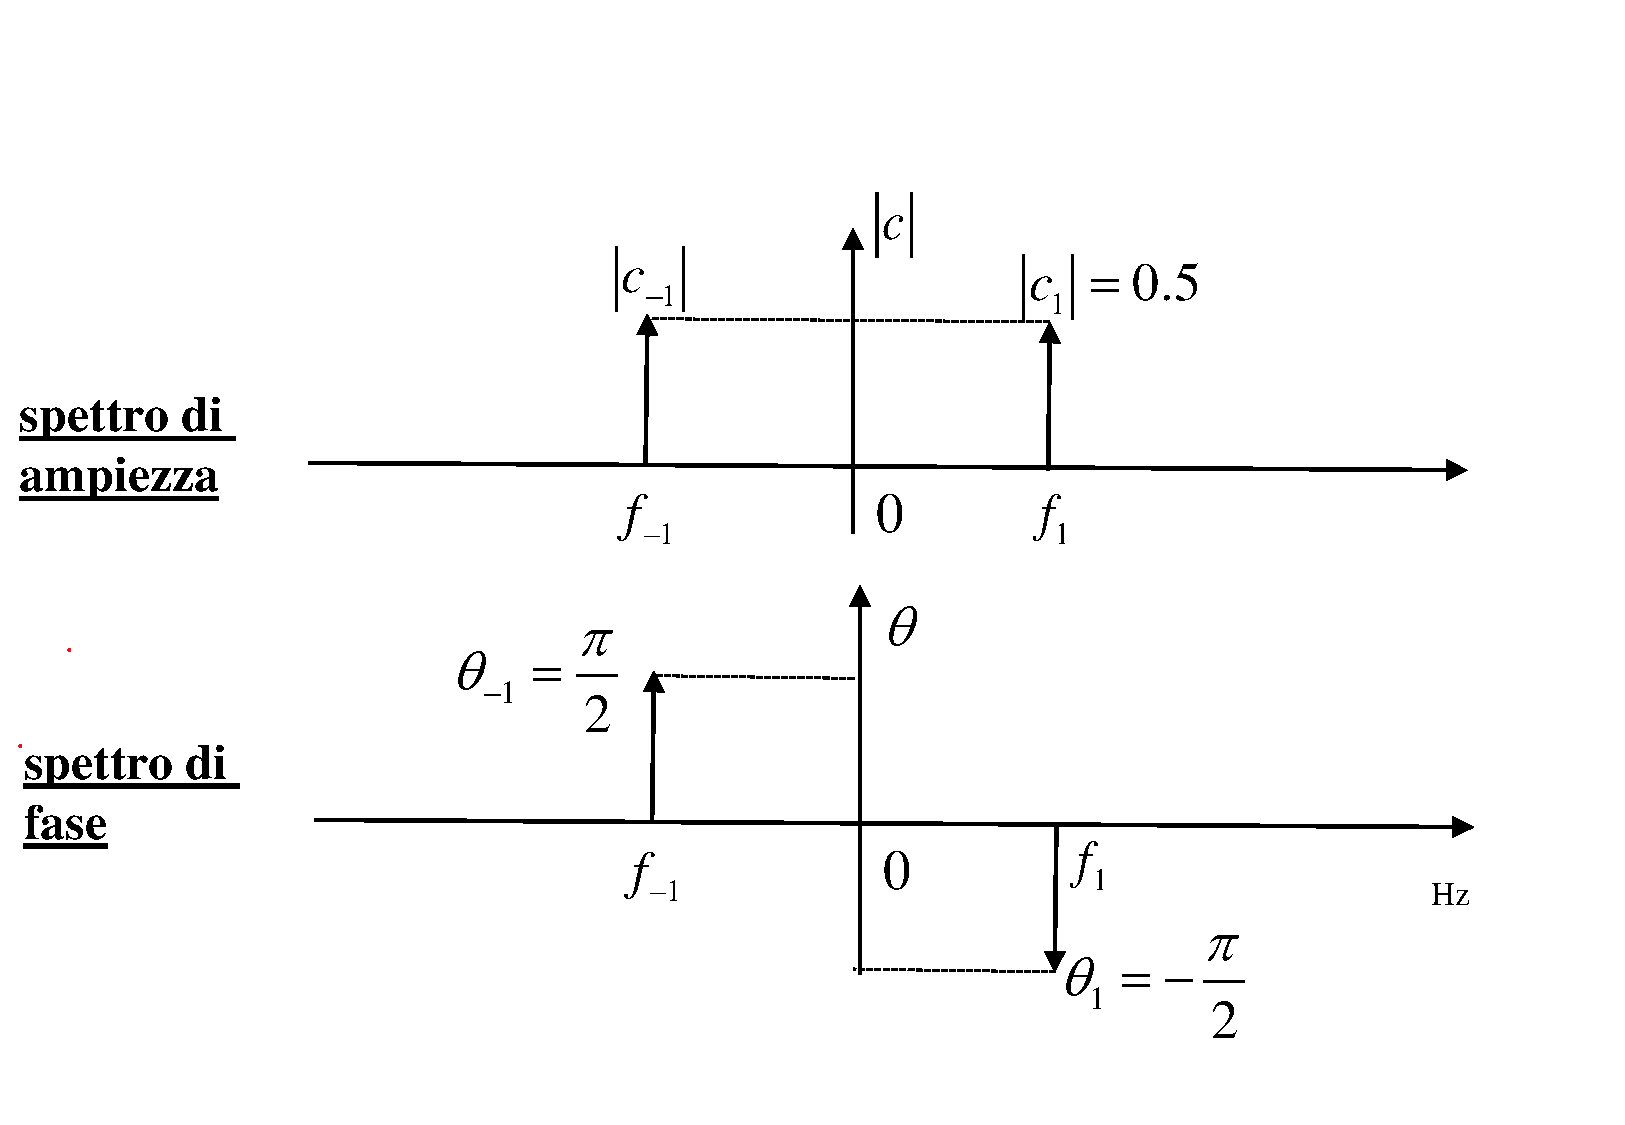
\includegraphics[width=0.9\textwidth]{img/fourier_spettro_di_ampiezza-e-fase.pdf}
		\caption{Spettro di ampiezza e di fase della funzione $\sin\left(2 \pi t\right)$.}
	\end{figure}

	\newpage
	
	\subsubsection{Proprietà della serie di Fourier}
	
	\noindent
	Lo \textbf{spettro di ampiezza e di fase} sono funzioni nel dominio delle frequenze che formano lo {\underline{\textcolor{Red3}{\textbf{spettro di Fourier}}}}. Lo spettro di Fourier per i segnali periodici gode delle \textbf{seguenti \underline{proprietà}}:
	
	\begin{itemize}
		\item Lo \textbf{spettro di ampiezza è \emph{simmetrico}} rispetto all'asse $y$;
		
		\item Lo \textbf{spettro di fase è \emph{antisimmetrico}} rispetto all'asse $y$;
		
		\item Se i coefficienti $c_{n}$ sono reali, \textbf{non esiste lo spettro di fase};
		
		\item Entrambe gli spettri sono funzioni a pettine\label{funzioni a pettine}, definite su frequenze multiple rispetto a quella fondamentale:
		
		\begin{equation*}
			\left\{\dfrac{2 \pi n}{T}\right\}_{n \in \mathbb{Z}} = \left\{f_{0} \cdot n\right\}_{n \in \mathbb{Z}} \equiv \left\{f_{n}\right\}_{n \in \mathbb{Z}}
		\end{equation*}
	\end{itemize}

	\newpage
	
	\subsection{Trasformata di Fourier continua} \label{trasformata di fouerier continua}
	
	\subsubsection{Trasformata di Fourier}
	
	Sia $f\left(t\right)$ un \textbf{segnale reale continuo} $f:\mathbb{R} \rightarrow \mathbb{R}$ periodico o non, si definisce la \textcolor{Red3}{\textbf{Trasformata di Fourier}} (TdF) $\mathcal{F}\left(f\left(t\right)\right) = F\left(\mu\right)$ il segnale $\mathcal{F}: \mathbb{R} \rightarrow \mathbb{C}$:
	
	\begin{equation*}
		\mathcal{F}\left(f\left(t\right)\right) = F\left(\mu\right) = \int_{-\infty}^{+\infty} f\left(t\right) e^{-j 2 \pi \mu t} \: \mathrm{d}t
	\end{equation*}

	\noindent
	L'\textbf{unità frequenziale} $\mu$ è l'angolo di $\frac{n}{T}$ della serie di Fourier (per esempio, con $n = 1$, $T = 1$ sec. $\rightarrow \mu = 1 \text{ sec.}^{-1} = 1$ Hz).\newline
	
	\noindent
	La Trasformata di Fourier esiste se $f\left(t\right)$ è un \textbf{segnale di energia}. Condizione sufficiente e non necessaria perché altri segnali ammettono la TdF.
	
	\subsubsection{Trasformata di Fourier inversa}
	
	Sia $F\left(\mu\right)$ la trasformata di Fourier di un segnale $f: \mathbb{R} \rightarrow \mathbb{R}$. Si definisce la \textcolor{Red3}{\textbf{trasformata di Fourier inversa}} il segnale $\mathcal{F}^{-1} \left(F\left(\mu\right)\right) = f\left(t\right)$:
	
	\begin{equation*}
		\mathcal{F}^{-1} = \left(F\left(\mu\right)\right) = f\left(t\right) = \int_{-\infty}^{+\infty} F\left(\mu\right) e^{j 2 \pi \mu t} \: \mathrm{d}\mu
	\end{equation*}

	\noindent
	La trasformata di Fourier restituisce, per una data frequenza $\mu$, un coefficiente di \dquotes{presenza} $F\left(\mu\right)$. Infatti, la sua inversa \textbf{\underline{permette di ricostruire $f$ a partire da $F$}}.
	
	\begin{figure}[!htp]
		\centering
		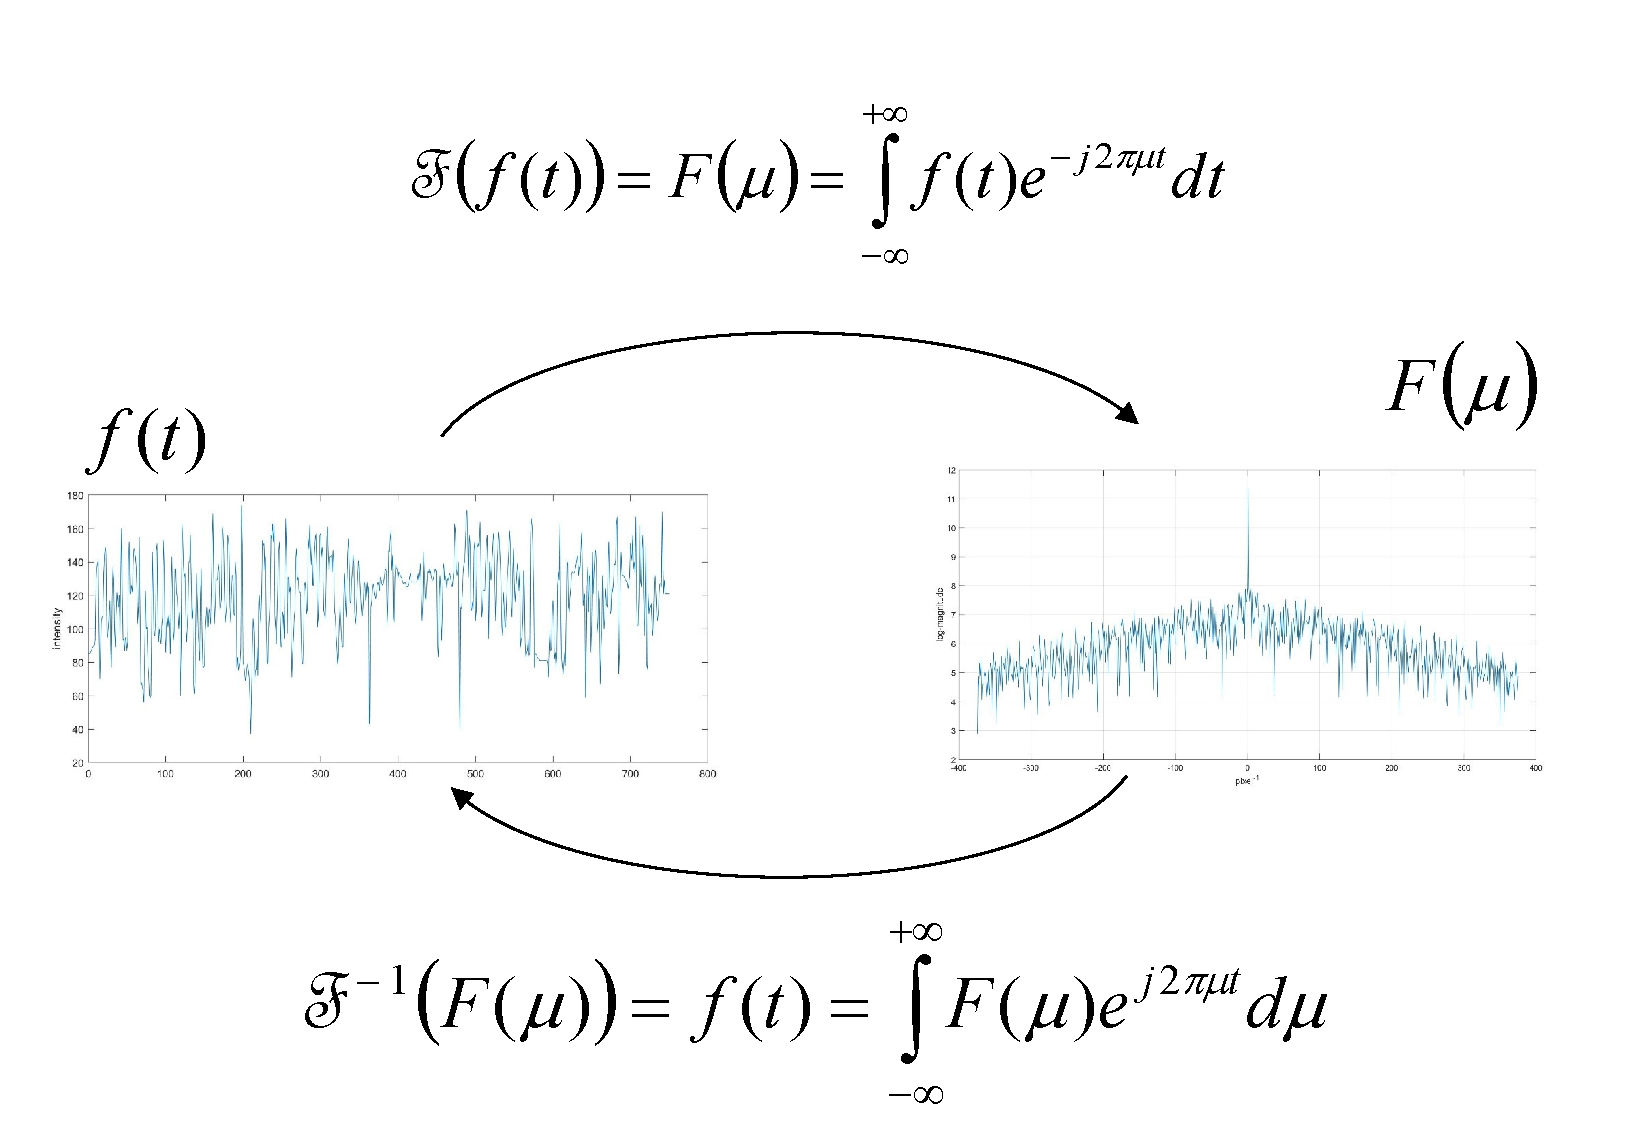
\includegraphics[width=1\textwidth]{img/trasformata_fourier1.pdf}
		\caption{(Anti)Trasformata di Fourier su un segnale $f\left(t\right)$.}
	\end{figure}

	\newpage

	\noindent
	Nel caso in cui il segnale $f\left(t\right)$ non è reale, la trasformata è complessa:
	
	\begin{itemize}
		\item $t$ rappresenta il \textbf{\underline{tempo}} (in secondi), allora $\mu$ rappresenta gli \textbf{Hertz}, cioè $\frac{\text{numero cicli}}{\text{secondi}}$;
		
		\item $t$ rappresenta lo \textbf{\underline{spazio}} (in metri), allora $\mu$ rappresenta la \textbf{frequenza spaziale}, cioè $\frac{\text{numero cicli}}{\text{metri}}$
	\end{itemize}

	\noindent
	Mentre nella serie di Fourier le funzioni rappresentate negli spettri di ampiezza e di fase erano a \dquotes{pettine} (paragrafo~\ref{funzioni a pettine}), in questo caso le funzioni sono solitamente continue, nello spettro di ampiezza, o continue a tratti:
	
	\begin{figure}[!htp]
		\centering
		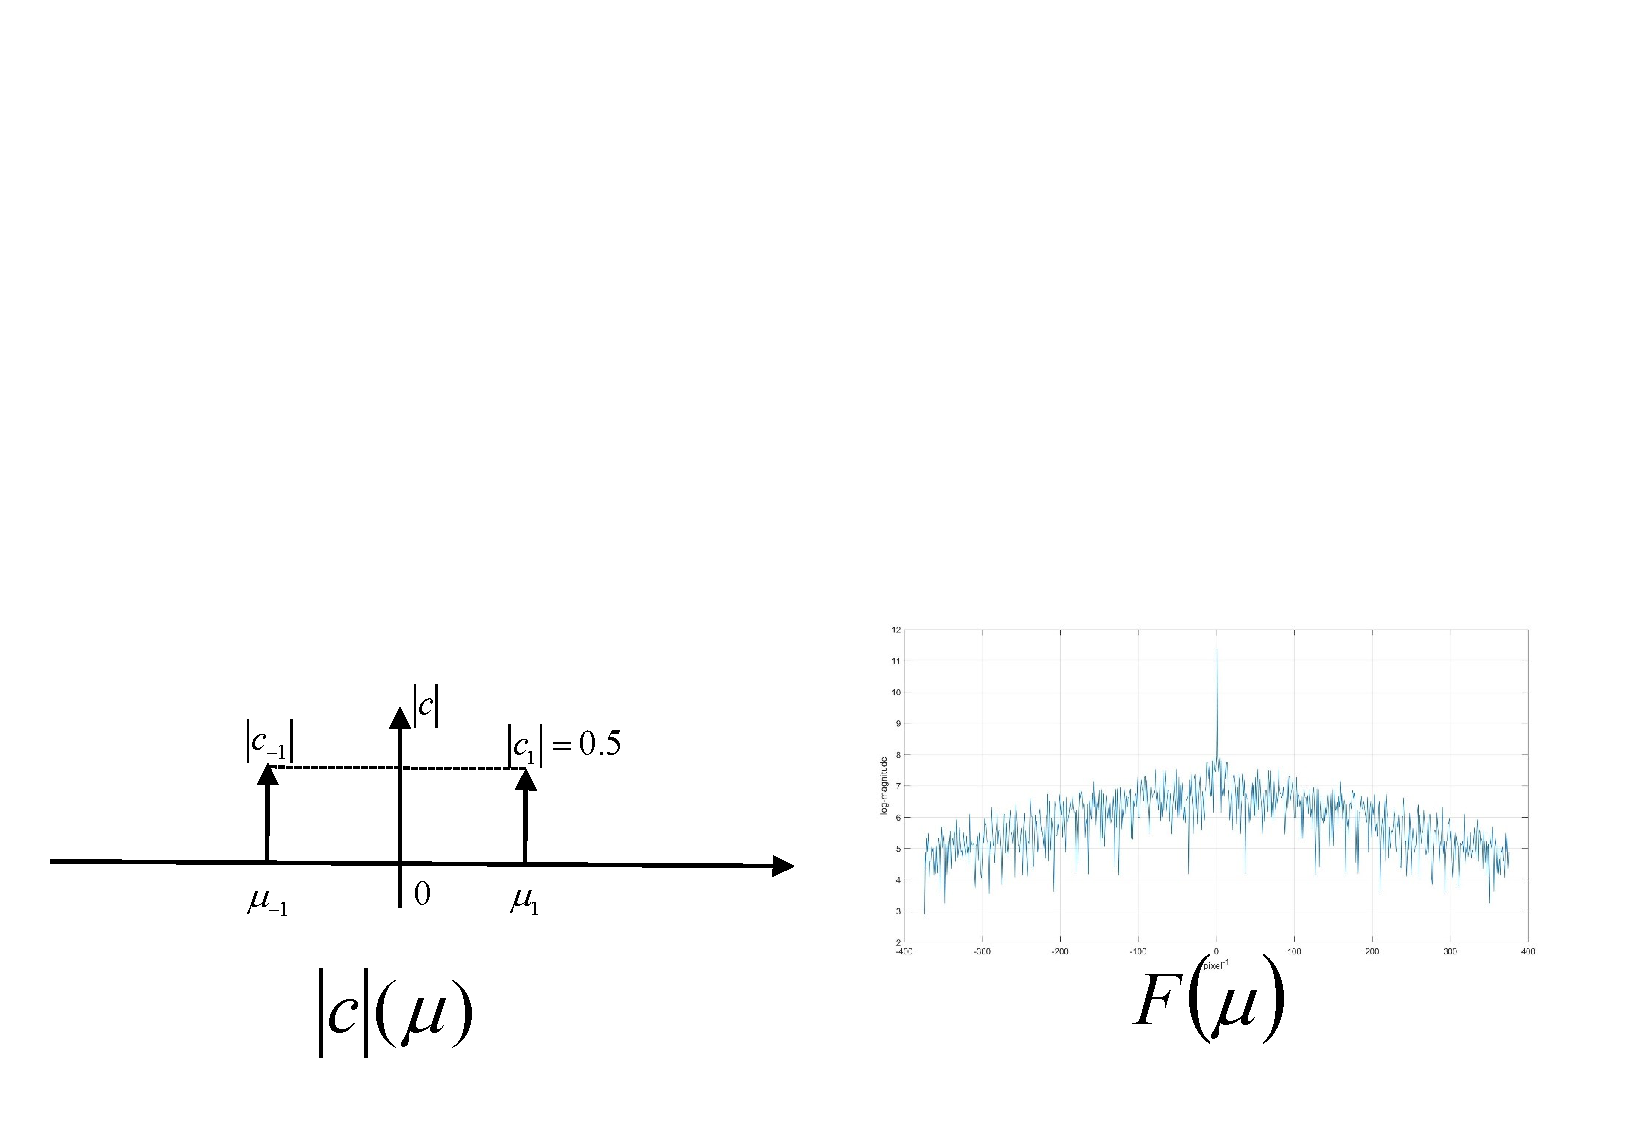
\includegraphics[width=0.9\textwidth]{img/trasformata_fourier2.pdf}
		\caption{Esempio di spettro di ampiezza.}
	\end{figure}
	
	\newpage
	
	\subsubsection{Proprietà della trasformata di Fourier}
	
	\begin{itemize}[label=\ding{42}]
		\item \textcolor{Red3}{\textbf{\underline{Linearità}}}
			\begin{equation*}
				a_{1} f_{1}\left(t\right) + a_{2}f_{2}\left(t\right) \hspace{1em} \xrightarrow{\mathcal{F}} \hspace{1em} a_{1}F_{1}\left(\mu\right) + a_{2}F_{2}\left(\mu\right)
			\end{equation*}
		
		\item \textcolor{Red3}{\textbf{\underline{Scalatura temporale}}}
			\begin{equation*}
				z\left(t\right) = f\left(at\right) \hspace{1em} \xrightarrow{\mathcal{F}} \hspace{1em} Z\left(\mu\right) = \dfrac{1}{a} \: F\left(\dfrac{\mu}{a}\right)
			\end{equation*}
		
		\item \textcolor{Red3}{\textbf{\underline{Dualità}}}
			\begin{gather*}
				f\left(t\right) \hspace{1em} \xrightarrow{\mathcal{F}} \hspace{1em} F\left(\mu\right) \\
				F\left(t\right) \hspace{1em} \xrightarrow{\mathcal{F^{-1}}} \hspace{1em} f\left(-\mu\right)
			\end{gather*}
			N.B. derivando la forma analitica per una trasformata, la sua antitrasformata ne produce un'altra con segno opposto.
			
		\item \textcolor{Red3}{\textbf{\underline{Time shift}}}
			\begin{equation*}
				\begin{matrix}
					\mathcal{F}\left(f\left(t-t_{0}\right)\right) & = & \displaystyle \int_{-\infty}^{+\infty} f\left(t-t_{0}\right) e^{-j 2 \pi \mu t} \: \mathrm{d}t \\
					\\
					& = & \displaystyle \int_{-\infty}^{+\infty} f\left(u\right) e^{-j 2 \pi \mu \left(u + t_{0}\right)} \: \mathrm{d}u \\
					\\
					& = & \displaystyle \int_{-\infty}^{+\infty} f\left(u\right) e^{-j 2 \pi \mu u} e^{-j 2 \pi \mu t_{0}} \: \mathrm{d}u \\
					\\
					& = & \displaystyle e^{-j 2 \pi \mu t_{0}} \: \int_{-\infty}^{+\infty} f\left(u\right) e^{-j 2 \pi \mu u} \: \mathrm{d}u \\
					\\
					& = & F\left(\mu\right) e^{\overbrace{- j 2 \pi \mu t_{0}}^{fase}}
				\end{matrix}
			\end{equation*}
	\end{itemize}

	\newpage
	
	\subsubsection{Trasformata di Fourier di una box}
	
	La trasformata di Fourier di una box (paragrafo~\ref{funzione box e impulso di Dirac}) è la seguente:
	
	\begin{equation*}
		\mathcal{F}\left(f\left(t\right)\right) = \int_{-\infty}^{+\infty} A \Pi \left(\dfrac{t}{w}\right) e^{-j 2 \pi \mu t} \: \mathrm{d}t = F\left(\mu\right)
	\end{equation*}

	\noindent
	Il \textbf{\underline{risultato corrisponde alla funzione}} $\mathrm{sinc}$:
	
	\begin{equation*}
		f\left(\mu\right) = Aw \cdot \mathrm{sinc }\left(\mu w\right)
	\end{equation*}
	
	\noindent
	Dove la funzione $\mathrm{sinc}$ è uguale a:
	
	\begin{equation*}
		\mathrm{sinc} = \dfrac{\sin\left(\pi \mu w\right)}{\pi \mu w}
	\end{equation*}

	\noindent
	Per ripassare la funzione $\mathrm{sinc}$, si rimanda al paragrafo~\ref{funzione sinc}. Tuttavia, si ricorda che la sua forma generale è del tipo:
	
	\begin{equation*}
		\mathrm{sinc} \left(m\right) = \dfrac{\sin \left(\pi m\right)}{\pi m}
	\end{equation*}

	\noindent
	E risultata uguale a:
	
	\begin{itemize}
		\item $\mathrm{sinc}\left(0\right) = 1$
		\item $\mathrm{sinc}\left(m\right) = 0 \hspace{1em} \forall m \in \mathbb{Z}$
	\end{itemize}

	\noindent
	Prima di concludere, si ricorda che:
	
	\begin{itemize}[label=\ding{43}]
		\item All'\textbf{aumentare} della \textbf{larghezza} della box, la funzione $\mathrm{sinc}$ tenderà a \textbf{stringersi};
		
		\item La box è \textbf{limita}, invece la $\mathrm{sinc}$ è \textbf{infinita} a destra e sinistra, anche se il termine al denominatore attenua il valore della funzione comportando un limite a $0$.
			
		\item In sintesi, la TdF di una box è:
			\begin{equation*}
				\Pi\left(\dfrac{t}{w}\right) \hspace{1em} \xrightarrow{\mathcal{F}} \hspace{1em} w \cdot \mathrm{sinc} \left(\mu w\right)
			\end{equation*}
	\end{itemize}

	\begin{figure}[!htp]
		\centering
		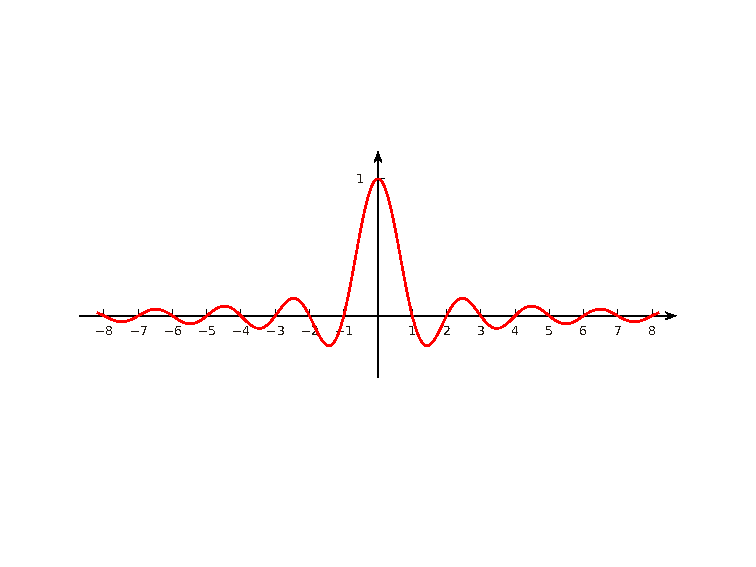
\includegraphics[width=0.8\textwidth]{img/sinc.pdf}
		\caption{Grafico della funzione sinc.}\label{grafico sinc}
	\end{figure}

	\newpage

	\subsubsection[Trasformata di Fourier di un $\mathrm{sinc}$]{Trasformata di Fourier di un $\boldsymbol{\mathrm{sinc}}$}
	
	La trasformata di Fourier di un segnale $\mathrm{sinc}$ (segnale rappresentato in figura~\ref{grafico sinc}) è la seguente:
	
	\begin{equation*}
		\mathcal{F}\left(f\left(t\right)\right) = \int_{-\infty}^{+\infty} \mathrm{sinc}\left(tw\right) e^{-j 2 \pi \mu t} \: \mathrm{d}t = F\left(\mu\right)
	\end{equation*}

	\noindent
	Dato che la TdF di una box è:
	
	\begin{equation*}
		\Pi\left(\dfrac{t}{w}\right) \hspace{1em} \xrightarrow{\mathcal{F}} \hspace{1em} w \cdot \mathrm{sinc} \left(\mu w\right)
	\end{equation*}

	\noindent
	Al contrario, si ottiene la \textbf{\underline{trasformata di Fourier di un $\mathrm{sinc}$}}:
	
	\begin{equation*}
		\mathrm{sinc}\left(tw\right) \hspace{1em} \xrightarrow{\mathcal{F}} \hspace{1em} \dfrac{1}{w} \Pi \left(-\dfrac{\mu}{w}\right) = \dfrac{1}{w} \cdot \Pi \left(\dfrac{\mu}{w}\right)
	\end{equation*}

	\newpage

	\subsubsection{Trasformata di Fourier di un impulso}
	
	La trasformata di Fourier di un impulso\footnote{Definizione di impulso al paragrafo~\ref{funzione box e impulso di Dirac}.} è la seguente:
	
	\begin{equation*}
		\mathcal{F}\left(f\left(t\right)\right) = F\left(\mu\right) = \int_{-\infty}^{+\infty} \delta\left(t\right) e^{-j 2 \pi \mu t} \: \mathrm{d}t
	\end{equation*}

	\noindent
	Il risultato della trasformata di Fourier di un impulso è molto semplice grazie alle sue proprietà. Infatti, il risultato è uguale a:
	
	\begin{equation*}
		\int_{-\infty}^{+\infty} \delta\left(t\right) e^{-j 2 \pi \mu t} \: \mathrm{d}t = \int_{-\infty}^{+\infty} \delta\left(0\right) e^{-j 2 \pi \mu 0} \: \mathrm{d}t = 1
	\end{equation*}

	\noindent
	La proprietà che consente di ottenere il risultato uguale a $1$ è la seguente:
	
	\begin{equation*}
		\delta\left(t\right) =
		\begin{cases}
			\infty  & \text{se } t = 0 \\
			0		& \text{se } t \ne 0
		\end{cases}
		\hspace{2em} \longrightarrow \hspace{2em}
		\int_{-\infty}^{+\infty}\delta\left(t\right)\mathrm{d}t = 1
	\end{equation*}

	\noindent
	\textbf{\underline{N.B. In questo caso è rappresentabile solo lo spettro di ampiezza!}}\newline
	
	\noindent
	Analogamente, con un impulso centrato in $t_{0}$, quindi non nell'origine:
	
	\begin{equation*}
		\mathcal{F}\left(f\left(t\right)\right) = F\left(\mu\right) = \int_{-\infty}^{+\infty} \delta\left(t-t_{0}\right) e^{-j 2 \pi \mu t} \: \mathrm{d}t = e^{-j 2 \pi \mu t_{0}}
	\end{equation*}

	\noindent
	Il risultato è stato ottenuto grazie alla proprietà di setacciamento (definita a pagina~\pageref{setacciamento}). Tuttavia, in questo caso i valori non sono più reali ma complessi.
	
	\newpage
	
	\subsubsection{Trasformata di Fourier di un treno di impulsi}
	
	Data la definizione di treno di impulsi (funzione definita nel paragrafo~\ref{treno_di_impulsi}):
	
	\begin{equation*}
		S_{\Delta T}\left(t\right) = \sum_{n = -\infty}^{+\infty} \delta\left(t - n\Delta T\right) \hspace{1em} n \in \mathbb{Z}
	\end{equation*}

	\noindent
	Si ottiene la sua relativa trasformata di Fourier:
	
	\begin{equation*}
		\mathcal{F}\left(S_{\Delta T}\left(t\right)\right) = \int_{-\infty}^{+\infty} S_{\Delta T}\left(t\right) e^{-j 2 \pi \mu t}\: \mathrm{d}t = F\left(\mu\right)
	\end{equation*}

	\noindent
	Tralasciando i vari calcoli numerici per arrivare al risultato, si può scrivere la trasformata di Fourier in maniera più semplice:
	
	\begin{equation*}
		S_{\Delta T}\left(t\right) \hspace{2em} \xrightarrow{\mathcal{F}} \hspace{2em} \sum_{n = -\infty}^{+\infty} \dfrac{1}{\Delta T} \delta\left(\mu - \dfrac{n}{\Delta T}\right)
	\end{equation*}

	\newpage
	
	\subsubsection{Sintesi}
	
	Qui di seguito si lascia un riassunto rapido delle trasformate di Fourier continue dei segnali più importanti.
	
	\begin{table}[!htbp]
		\centering
		\begin{tabular}{@{} l l c l @{}}
			\toprule
			Segnale & & & Trasformata di Fourier \\
			\midrule
			Box:				& $A\Pi\left(\dfrac{t}{w}\right)$	& $\xrightarrow{\mathcal{F}}$ & $Aw \cdot \mathrm{sinc}\left(\mu w\right)$ \\
			&&&\\
			Sinc:				& $\mathrm{sinc}\left(tw\right)$	& $\xrightarrow{\mathcal{F}}$ & $\dfrac{1}{w}\cdot\Pi \left(-\dfrac{\mu}{w}\right) = \dfrac{1}{w}\cdot \Pi\left(\dfrac{\mu}{w}\right)$ \\
			&&&\\
			Impulso:			& $\delta\left(t\right)$			& $\xrightarrow{\mathcal{F}}$ &
			$\begin{cases}
				1 						& \text{se valori reali}\\
				e^{-j 2 \pi \mu t_{0}}	& \text{se valori complessi}
			\end{cases}$ \\
			&&&\\
			Treno di impulsi:	& $S_{\Delta T}\left(t\right)$ 		& $\xrightarrow{\mathcal{F}}$ & $\displaystyle\sum_{n = -\infty}^{+\infty} \dfrac{1}{\Delta T} \cdot \delta \left(\mu - \dfrac{n}{\Delta T}\right)$ \\
			\bottomrule
		\end{tabular}
		\caption{Trasformate di Fourier dei segnali pù importanti.}
	\end{table}

	\newpage
	
	\subsection{Trasformata di Fourier a tempo discreto}\label{trasformata di fourier a tempo discreto}
	
	\subsubsection{Campionamento}
	
	Sia $f\left(t\right)$ un segnale reale continuo definito $f : \left] -\infty, + \infty \right[ \in \mathbb{R} \rightarrow \mathbb{R}$ (attenzione al dominion non limitato), anche non periodico:
	
	\begin{figure}[!htp]
		\centering
		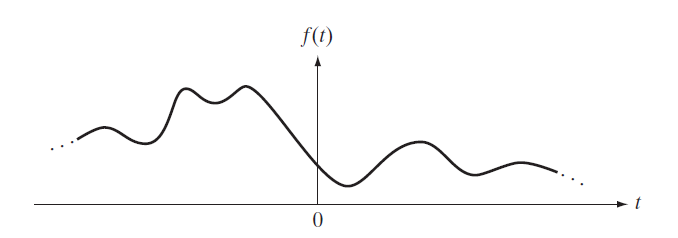
\includegraphics[width=0.65\textwidth]{img/campionamento_1.png}
	\end{figure}

	\noindent
	Questo tipo di segnale, per essere elaborato al computer deve essere \textbf{campionato} ad intervalli discreti. Per farlo, si prenda in considerazione il treno di impulsi:
	
	\begin{equation*}
		S_{\Delta T} \left(t\right) = \sum_{n = -\infty}^{+\infty} \delta\left(t - n\Delta T\right)
	\end{equation*}

	\noindent
	Con periodo $\Delta T$, ossia con \textbf{frequenza di campionamento} pari a: $\mu_{S} = \dfrac{1}{\Delta T}$

	\begin{figure}[!htp]
		\centering
		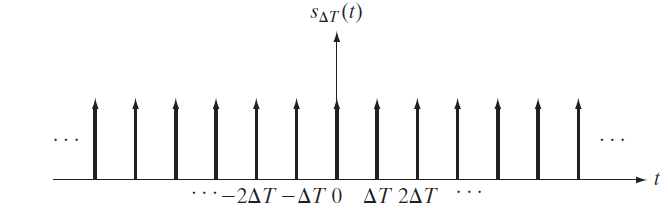
\includegraphics[width=0.65\textwidth]{img/campionamento_2.png}
	\end{figure}

	\noindent
	Si assuma che il treno di impulsi sia un \textbf{segnale discreto}. Matematicamente parlando, \textbf{campionare un segnale \underline{significa} moltiplicarlo per un treno di impulsi}:
	
	\begin{equation*}
		\tilde{f}\left(t\right) = f\left(t\right) \cdot S_{\Delta T}\left(t\right) = f\left(t\right) \cdot \sum_{n = -\infty}^{+\infty} \delta\left(t - n \Delta T\right)
	\end{equation*}

	\begin{figure}[!htp]
		\centering
		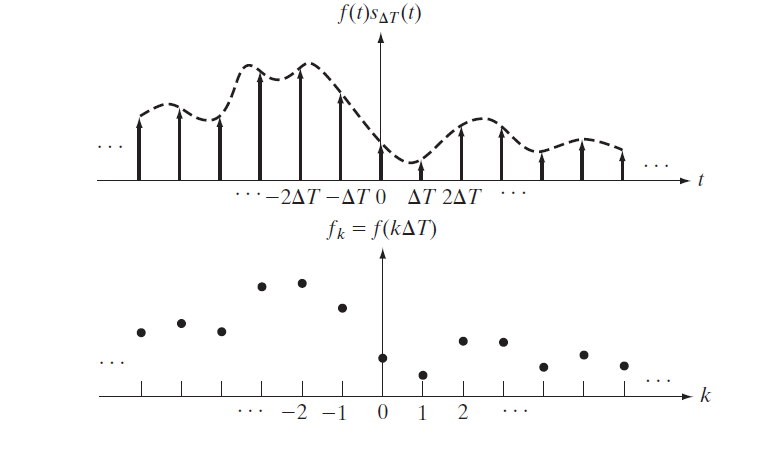
\includegraphics[width=0.65\textwidth]{img/campionamento_3.png}
	\end{figure}
	
	\newpage
	
	\subsubsection{Trasformata di Fourier a tempo discreto}
	
	Sia $F\left(\mu\right)$ la trasformata di Fourier di un segnale $f\left(t\right): \mathbb{R} \rightarrow \mathbb{R}$. Si considera $\tilde{f}\left(t\right)$ e si calcola la trasformata di Fourier $\tilde{F}\left(\mu\right)$ (entrambi sono a tempo discreto). Grazie alla convoluzione si ottiene:
	
	\begin{equation*}
		\tilde{F}\left(\mu\right) = \mathcal{F}\left\{\tilde{f}\left(t\right)\right\} = F\left(\mu\right) * S_{\Delta T}\left(\mu\right)
	\end{equation*}

	\noindent
	Si ricorda che:
	
	\begin{equation*}
		S_{\Delta T} \left(\mu\right) = \dfrac{1}{\Delta T} \sum_{n = -\infty}^{+\infty}\delta\left(\mu - \dfrac{n}{\Delta T}\right)
	\end{equation*}	

	\noindent
	E risolvendo la convoluzione, si ottiene che la \textcolor{Red3}{\textbf{\underline{trasformata di Fourier a tempo}}} \textcolor{Red3}{\textbf{\underline{discreto}}} corrisponde a:
	
	\begin{equation*}
		F\left(\mu\right) * S_{\Delta T}\left(\mu\right) = \int_{-\infty}^{+\infty} F\left(\tau\right) \cdot S_{\Delta T} \left(\mu - \tau\right) \: \mathrm{d}\tau = \dfrac{1}{\Delta T} \sum_{n = -\infty}^{+\infty} F \left(\mu - \dfrac{n}{\Delta T}\right)
	\end{equation*}

	\noindent
	Analizzando la formula si evidenziano alcuni termini:
	
	\begin{itemize}
		\item $F\left(\mu\right)$ è la trasformata di Fourier della funzione originale $f\left(t\right)$;
		
		\item $F\left(\mu - \dfrac{n}{\Delta T}\right)$ è la trasformata di Fourier della funzione originale $f\left(t\right)$ shiftato a destra di una quantità pari a $\dfrac{n}{\Delta T}$;
		
		\item $\dfrac{1}{\Delta T} \sum_{n = -\infty}^{+\infty} F \left(\mu - \dfrac{n}{\Delta T}\right)$ sono infinite copie dello spettro $F\left(\mu\right)$, ripetute ovviamente ogni $\dfrac{1}{\Delta T}$. \newline
		Inoltre, è un \textbf{segnale periodico} (nelle frequenze) di periodo $\dfrac{1}{\Delta T}$, ovvero si ripete ogni $\dfrac{1}{\Delta T}$ Hz.\newline
		La sua scalatura nell'ampiezza è pari a $\dfrac{1}{\Delta T}$ e rappresenta la T.d.F. a tempo discreto.
	\end{itemize}

	\newpage
	
	\subsubsection{Teorema del campionamento}
	
	Un \textbf{\underline{segnale reale continuo}} $f\left(t\right)$, limitato in banda, può essere \textbf{\underline{ricostruito}} \textbf{\underline{senza errori completamente dai suoi campioni}} se essi sono acquisiti con un tempo di campionamento $\Delta T$ tale per cui:
	
	\begin{equation*}
		\dfrac{1}{\Delta T} = \mu_{S} \ge 2 \mu_{\text{max}}
	\end{equation*}

	\noindent
	Ovvero se nel tempo si adotta una frequenza di campionamento $\dfrac{1}{\Delta T}$ almeno doppia rispetto alla frequenza massima del segnale $\mu_{\text{max}}$.\newline
	In altre parole, il teorema del campionamento afferma che tutte le proprietà di un segnale possono essere espresse usando dei campioni.\newline
	
	\noindent
	\textbf{\underline{Attenzione!}} L'espressione $\dfrac{1}{\Delta T}$ viene chiamata \textbf{\emph{frequenza di Nyquist}} e per frequenze minori si crea aliasing, fenomeno che impedisce la ricostruzione senza errori.
	
	\subsubsection{Considerazioni}
	
	Dal \textbf{\underline{punto di vista teorico}} la trasformata di Fourier a tempo discreto consente di ricostruire il segnale. Tuttavia, è impossibile implementarla in un computer poiché tende, come limiti, all'infinito e ci vorrebbe un numero infinito di campioni e di segnali di tipo $\mathrm{sinc}$.
	
	\newpage
	
	\subsection{Trasformata di Fourier discreta}\label{trasformata di fourier discreta}
	
	La trasformata di Fourier di un segnale reale continuo $f\left(t\right)$ di dominio illimitato e non periodico, campionato nel tempo con periodo di campionamento $\Delta T$, è una funzione continua, periodica (di periodo $\dfrac{1}{\Delta T}$) anch'essa di dominio illimitato:
	
	\begin{equation*}
		\tilde{f}\left(t\right) = f\left(t\right) \cdot \sum_{n = -\infty}^{+\infty}\delta\left(t - n\Delta T\right) \: \textcolor{Red3}{\overset{\mathcal{F}}{\longrightarrow}} \: \tilde{F}\left(\mu\right) = \dfrac{1}{\Delta T} \sum_{n = -\infty}^{+\infty} F\left(\mu - \dfrac{n}{\Delta T}\right)
	\end{equation*}

	\noindent
	Il \textbf{problema} di questa formulazione è data l'espressione analitica dello spettro, la quale suppone che si è a \textbf{conoscenza della T.d.F.} teorica $F$ \textbf{del segnale di partenza}. Questo, spesso, è molto difficile.\newline
	
	\noindent
	Si ricava dunque una \emph{forma più semplice} da manipolare. Essa consente di \textbf{costruire una rappresentazione spettrale a partire dai campioni della funzione originale} $f\left(t\right)$:
	
	\begin{equation*}
		\tilde{F}\left(\mu\right) = \sum_{n = -\infty}^{+\infty} f_{n} \: e^{-j 2 \pi \mu n \Delta T}
	\end{equation*}
	
	\noindent
	Al contrario, la prima formulazione era più chiara per comprendere il fatto che la T.d.F. di una funzione campionata genera delle repliche dello spettro originale $F\left(\mu\right)$.\newline
	
	\noindent
	L'equazione alternativa deve essere modificata, eseguendo un campionamento per il dominio spettrale, per poterla implementare su un computer. Per farlo, si prende in considerazione solo l'intervallo frequenziale da $0$ a $\dfrac{1}{\Delta T} = \mu_{S}$.
	
	\begin{figure}[!htp]
		\centering
		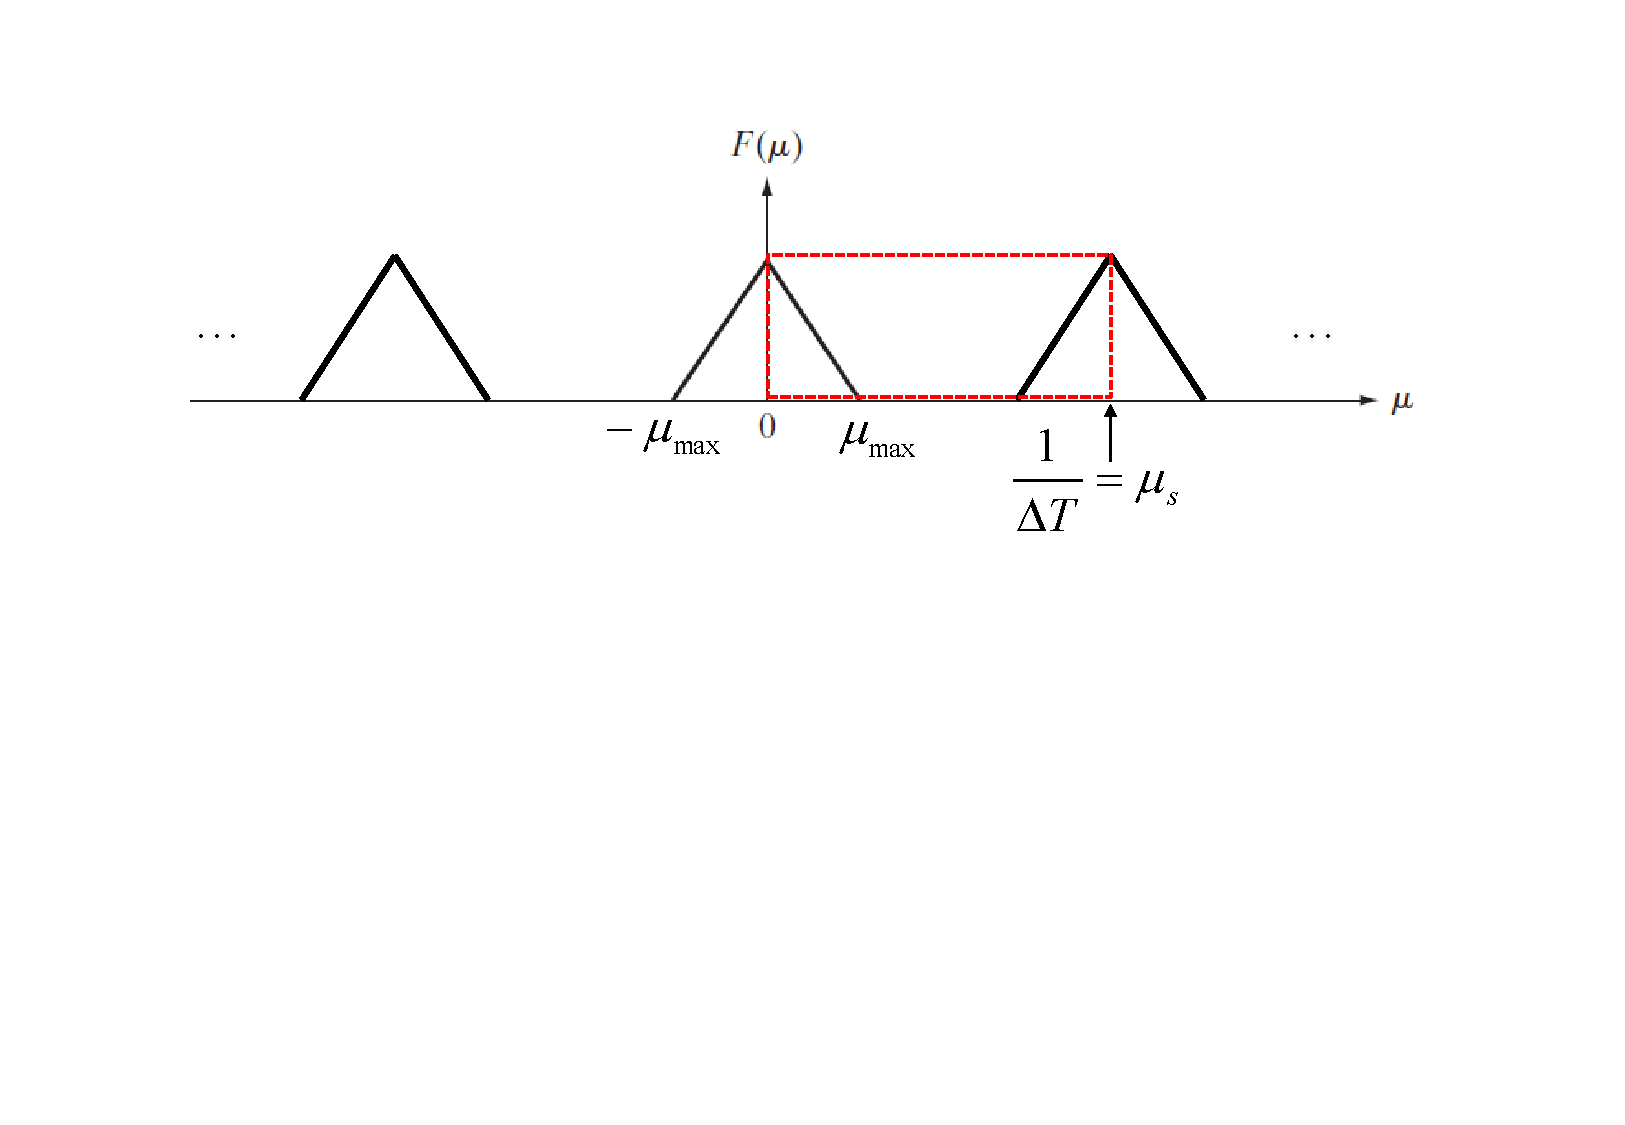
\includegraphics[width=0.7\textwidth]{img/trasformata_fourier_discreta1.pdf}
	\end{figure}

	\noindent
	Inoltre, si prendono in considerazione $M$ campioni tramite l'operazione di campionamento.
	
	\begin{figure}[!htp]
		\centering
		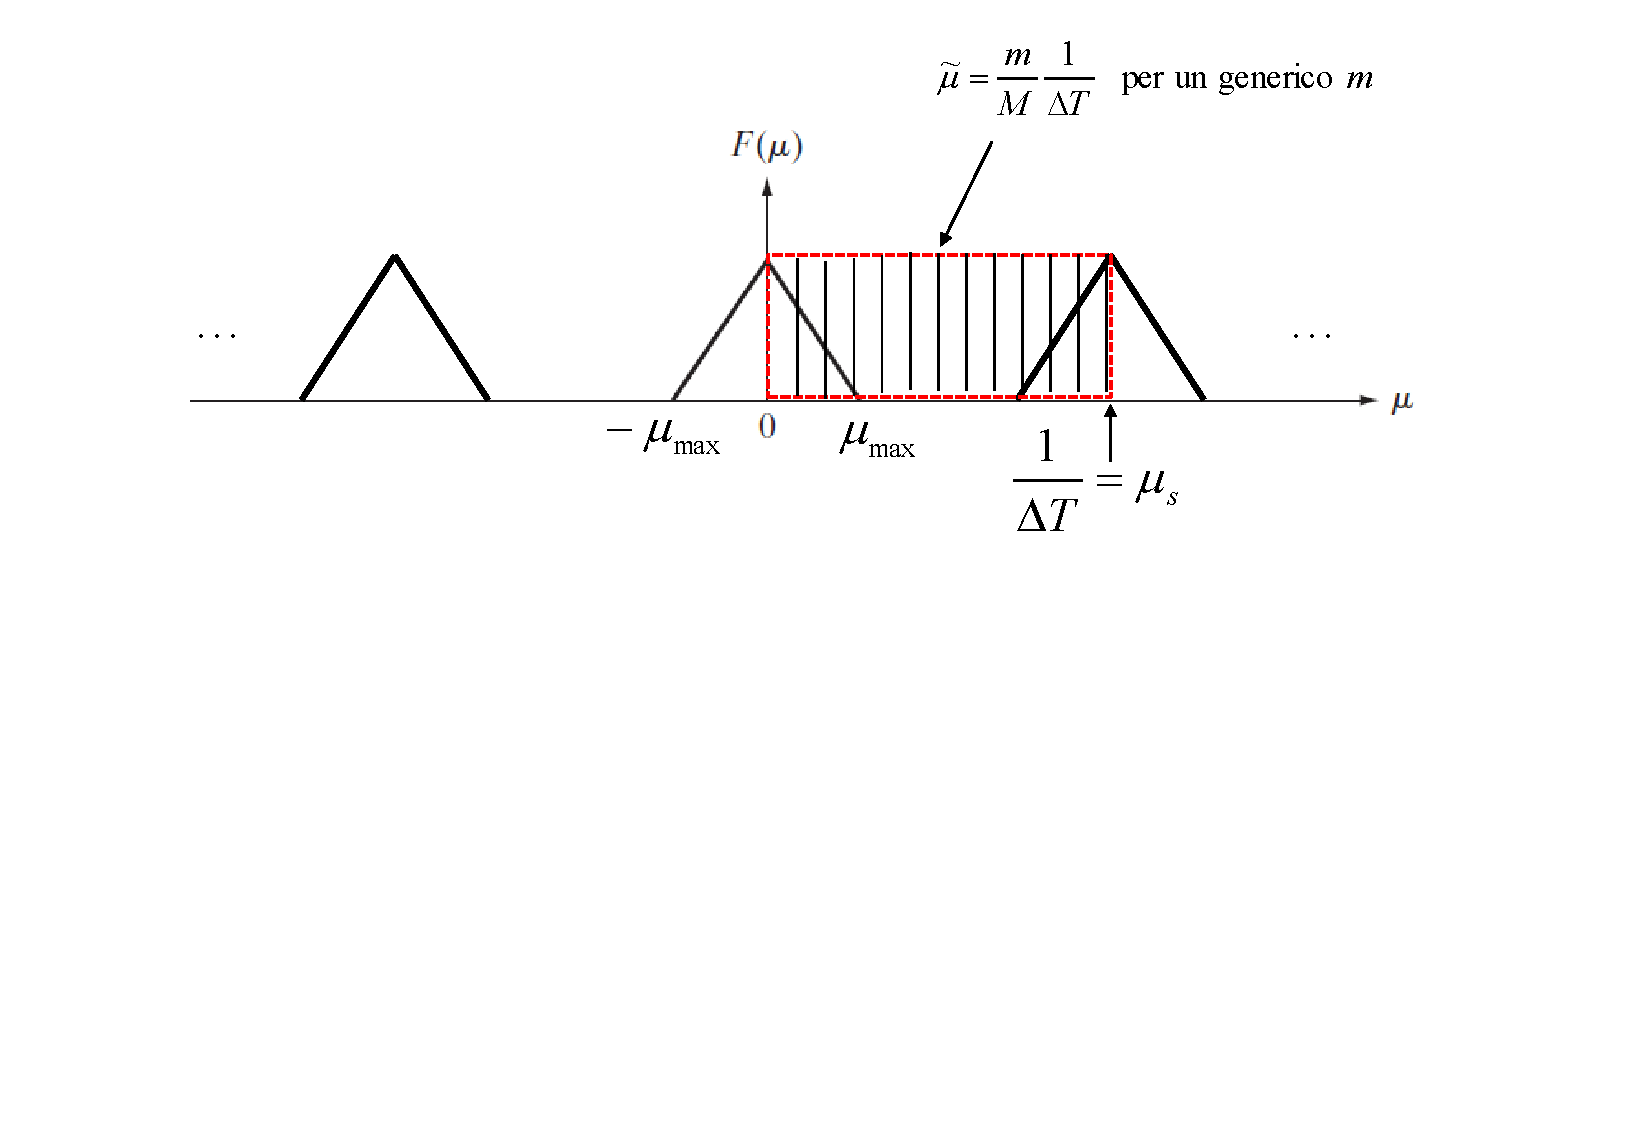
\includegraphics[width=0.7\textwidth]{img/trasformata_fourier_discreta2.pdf}
	\end{figure}

	\noindent
	In cui:
	
	\begin{equation*}
		\tilde{\mu} = \dfrac{m}{M} \cdot \dfrac{1}{\Delta T} \hspace{2em} \text{con } m = 0, ..., M-1 \text{ e dove } \dfrac{m}{M} \in \left[0,1 - \dfrac{1}{M}\right]
	\end{equation*}

	\noindent
	La $m$ indica il \textbf{range di variazione} degli indici dei campioni frequenziali. Calcolando la trasformata di Fourier a tempo discreto sui campioni $M$, si giunge alla \textcolor{Red3}{\textbf{\underline{forma finale della trasformata di Fourier discreta}}}:
	
	\begin{equation*}
		\tilde{F}\left(\tilde{\mu}\right) = \tilde{F}\left(\dfrac{m}{M} \cdot \dfrac{1}{\Delta T}\right) = \sum_{n = 0}^{M - 1} f_{n} e^{-j 2 \pi \frac{m}{M} n} \hspace{2em} \text{con } m = 0, ..., M - 1
	\end{equation*}

	\noindent
	La \textcolor{Red3}{\textbf{\underline{trasformata di Fourier discreta inversa}}}, ovvero l'antitrasformata:
	
	\begin{equation*}
		\tilde{f}\left(n \Delta T\right) = f\left(n \Delta T\right) = f_{n} = \dfrac{1}{M} \sum_{m = 0}^{M - 1} F_{m} e^{j 2 \pi \frac{m}{M} n}
	\end{equation*}

	\newpage
	
	\subsection{Riassunto Trasformate}
	
	Qui di seguito vengono rappresentate le trasformate più importanti.
	
	% TODO: finire la creazione della tabella con le T.d.F. più importanti
	
	\newpage
	
	\subsection{Domanda da esame}
	
	All'esame è possibile che sia richiesto come domanda: \dquotes{quali sono le trasformate di Fourier studiate durante il corso?}
	
	La risposta, anche se banale, è la seguente: le trasformate di Fourier studiate durante il corso sono $4$:
	
	\begin{enumerate}[label=\Roman*.]
		\item Serie di Fourier (paragrafo~\ref{serie di fourier})
		\item Trasformata di Fourier continua (paragrafo~\ref{trasformata di fouerier continua})
		\item Trasformata di Fourier a tempo discreto (paragrafo~\ref{trasformata di fourier a tempo discreto})
		\item Trasformata di Fourier discreta (paragrafo~\ref{trasformata di fourier discreta})
	\end{enumerate}

	% TODO: ricordati il todo
\end{document}